\documentclass[a4paper, 12pt, twoside, openright]{book}

% -------------------------------------------------------------------------
% GENERAL NOTES
% To compile this file, you need to have at least one citation and one defined acronym
% Define one citation in 'Sections/reference_list.bib' and use any of the \cite commands anywhere in the text to avoid errors
% Define one acronym in 'Sections/4.5-list_of_acronyms.tex' and use \an{defined-acronym} anywhere in the text to avoid errors
% -------------------------------------------------------------------------

% Configurations for the TeX template
% !TeX root = ..\Thesis.tex

% Encoding and Language
\usepackage[utf8]{inputenc}  % Input encoding, allows the use of UTF-8 characters
\usepackage[portuguese]{babel}  % Language support, here set to English
\usepackage[T1]{fontenc}     % Output font encoding, improves handling of special characters

% Mathematics
\usepackage{amsmath, amssymb}   % Basic math symbols and environments
\usepackage{dsfont}             % Double-struck fonts (e.g., for the indicator function)
\usepackage{bm}                 % Bold math symbols
\usepackage{mathrsfs}           % Additional math script fonts

% Graphics and Figures
\usepackage{graphicx}           % Include images and graphics
\usepackage{float}              % Improved control over float placement
%\floatstyle{boxed}             % Option for boxed floats (currently commented out)
\restylefloat{figure}           % Allows restyling of figure floats
\usepackage{subcaption}         % Sub-figures within a single figure
\usepackage[font={footnotesize,it}]{caption}  % Caption formatting, small and italic
\usepackage{adjustbox}          % Adjust size and alignment of content (e.g., images)


% Tables
% https://people.inf.ethz.ch/markusp/teaching/guides/guide-tables.pdf
\usepackage{booktabs}           % Professional-quality tables
\usepackage{threeparttable}     % Tables with notes below them
\usepackage{makecell}           % Customizable cell format in tables
\usepackage{multicol, multirow} % Multi-column and multi-row cells in tables
\usepackage[table]{xcolor}      % Color support in tables (and elsewhere)

% Text Formatting and Styling
\usepackage{color}              % Colored text
\usepackage{url}                % Proper formatting of URLs
\usepackage{fancyhdr}           % Custom headers and footers
\usepackage[procnames]{listings} % Code listings with syntax highlighting
\usepackage{lstautogobble}      % To remove empty lines at the end of listing envs
\usepackage[onehalfspacing]{setspace}  % Line spacing adjustments (1.5 spacing here)
\usepackage[nottoc]{tocbibind}  % Add bibliography/index to the Table of Contents

% Float Management
\usepackage{flafter}            % Prevents floats from appearing before their references
\usepackage[section]{placeins}  % Prevents floats from leaving their section

% Layout and Geometry
\usepackage[a4paper, left=3cm, right=2cm, top=3cm, bottom=2cm]{geometry}  % Page margins
\usepackage[space]{grffile}     % Allows spaces in graphic file names
%\usepackage{showframe}         % Displays the layout frames (currently commented out)
%\usepackage{fullpage}          % Use full page layout (currently commented out)
%\usepackage{comment}           % Allows commenting out large sections of text

% Special Features
\usepackage{eso-pic}            % Add background picture to pages (e.g., title page)
\usepackage{natbib}             % Bibliography and citations with NatBib
\usepackage{acro}               % Enables the definition and management of acronyms
\usepackage{tcolorbox}          % For bounding boxes
\usepackage{siunitx}            % Physical units
%\usepackage[printonlyused, withpage]{acronym} % Enables the definition and management of acronyms (another way)
%\usepackage{icomma}            % Adjust spacing after commas in math mode (currently commented out)
%\usepackage{array}             % Advanced table options (currently commented out)
%\setlength{\extrarowheight}{.5ex}  % Extra row height for tables (use with array package)
%\usepackage[outline]{contour}  % Outlined text (currently commented out)
\usepackage{layouts} 
\usepackage{tikz}
\usetikzlibrary{shapes, arrows.meta, positioning, shapes.geometric, fit}

\usepackage[indent=1.5cm]{parskip} % 1.5cm identation, following ABNT rules

% \newcommand{\ra}[1]{\renewcommand{\arraystretch}{#1}}  % Adjusts row spacing in tables

% ------------------------------------------------------------------------------
% Optional Packages
% ------------------------------------------------------------------------------
% Uncomment if you want to use these features

% Minted: Code listings with syntax highlighting
%\usepackage{minted}
%\usemintedstyle{pastie}  % Pastie style for minted code blocks

% Line Numbers
\usepackage{lineno}
% \linenumbers  % Enables line numbering, comment this line to remove them

% ------------------------------------------------------------------------------
% Define dynamic chapter titles based on language
% ------------------------------------------------------------------------------
\providecommand{\chapternameintro}{%
  \iflanguage{portuguese}{Introdução}{Introduction}}
\providecommand{\chapternamedatabase}{%
  \iflanguage{portuguese}{Base de dados fotométricos}{Data base}}
\providecommand{\chapternameanalysis}{%
  \iflanguage{portuguese}{UCDs na região de Fornax}{Analysis}}
\providecommand{\chapternamespectra}{%
  \iflanguage{portuguese}{Espectroscopia de uma amostra de candidatas a UCDs em Fornax}{Spectra}}
\providecommand{\chapternamespectraemission}{%
  \iflanguage{portuguese}{Objetos compactos com emissão}{Compact objects with emission lines}}
\providecommand{\chapternameconclusions}{%
  \iflanguage{portuguese}{Conclusões}{Conclusions}}
\providecommand{\chapternamefuture}{%
  \iflanguage{portuguese}{Perspectivas futuras}{Future perspectives}}
\providecommand{\chapternameacronyms}{%
  \iflanguage{portuguese}{Lista de Acrônimos}{List of Acronyms}}
\providecommand{\chapternameappendix}{%
  \iflanguage{portuguese}{Observações de candidatas a UCDs com o Gemini Sul}{Appendix}}

% ------------------------------------------------------------------------------
% Listing theme
% ------------------------------------------------------------------------------
% https://tex.stackexchange.com/questions/235731/listings-syntax-for-literate

\definecolor{codegreen}{rgb}{0,0.6,0}
\definecolor{codegray}{rgb}{0.5,0.5,0.5}
\definecolor{codepurple}{rgb}{0.58,0,0.82}
\definecolor{backcolour}{rgb}{0.97,0.97,0.97}
 
\lstdefinestyle{mystyle}{
    morekeywords={access,and,break,class,continue,def,del,elif,else,except,exec,
    finally,for,from,global,if,import,in,is,lambda,not,or,pass,print,raise,
    return,self,try,while},
    morekeywords=[2]{abs,all,any,basestring,bin,bool,bytearray,callable,chr,
    classmethod,cmp,compile,complex,delattr,dict,dir,divmod,enumerate,eval,
    execfile,file,filter,float,format,frozenset,getattr,globals,hasattr,hash,
    help,hex,id,input,int,isinstance,issubclass,iter,len,list,locals,long,map,
    max,memoryview,min,next,object,oct,open,ord,pow,property,range,raw_input,
    reduce,reload,repr,reversed,round,set,setattr,slice,sorted,staticmethod,str,
    sum,super,tuple,type,unichr,unicode,vars,xrange,zip,apply,buffer,coerce,
    intern},
    backgroundcolor=\color{backcolour},
    commentstyle=\color{codegreen},
    keywordstyle=\color{magenta},
    numberstyle=\tiny\color{codegray},
    stringstyle=\color{codepurple},
    basicstyle=\scriptsize\ttfamily,
    breakatwhitespace=false,
    breaklines=true,
    captionpos=b,
    keepspaces=true,
    numbers=left,
    numbersep=10pt,
    showspaces=false,
    showstringspaces=false,
    showtabs=false,
    tabsize=2,
    frame=single,
    frameround={t}{t}{t}{t},
    framexleftmargin=6mm,
    xleftmargin=20pt,
    xrightmargin=3pt
    }
\lstset{style=mystyle}

% ------------------------------------------------------------------------------
% Custom Page Elements and Layout Adjustments
% ------------------------------------------------------------------------------

% Create a new environment that defines a right-aligned box
\newenvironment{rightbox}[1]
 {\itemize[
    nosep,
    leftmargin=\dimexpr\textwidth-#1\relax,
    rightmargin=0pt,
    itemindent=\parindent,
    listparindent=\parindent,
  ]\item[]\relax}
 {\enditemize}

% Command to create a blank page
\newcommand\blankpage{%
    \null
    \thispagestyle{empty}%
    \addtocounter{page}{-1}%
    \newpage
}

% Fancy Header Configuration
\fancyhead{}  % Clear default header
\fancyfoot{}  % Clear default footer
\fancyhead[RO,LE]{\thepage}  % Page number on the right for odd pages and left for even pages
\fancyhead[CE]{\nouppercase\leftmark}  % Section title centered on even pages
\fancyhead[CO]{\nouppercase\rightmark} % Chapter title centered on odd pages
\pagestyle{fancy}  % Apply fancyhdr configuration

% Customization of section marks in headers
\renewcommand{\sectionmark}[1]{%
    \markright{\scriptsize{\slshape{\fontsize{10}{12} \selectfont Section \thesection.\ #1}}}
}
\renewcommand{\headrulewidth}{0.7pt}  % Line width for header rule
\setlength{\headheight}{14pt}  % Adjust header height

% ------------------------------------------------------------------------------
% Custom Commands for Color
% ------------------------------------------------------------------------------

\definecolor{lightgray}{gray}{0.7}  % Define light gray color
\definecolor{gray75}{gray}{0.75}  % Define 75% gray color

% ------------------------------------------------------------------------------
% Page Layout and Section Formatting
% ------------------------------------------------------------------------------

\usepackage{emptypage}  % Suppresses page numbers on empty pages
\usepackage{titlesec, blindtext}  % Customization of section titles

% Customization of the Table of Contents
\renewcommand\contentsname{Table of Contents}
\titleformat{\chapter}[display]  % Format for chapters with number
{\bfseries\Huge}
{{\chaptertitlename} \large\thechapter}
{2ex}
{\titlerule\vspace{2ex}}

\titleformat{name=\chapter,numberless}[display]  % Format for unnumbered chapters
{\bfseries\Huge}
{\color{gray75}{\titlerule[0.8pt]}}
{-8ex} % Should be -7ex if not using parskip
{\bfseries\Huge}[]

% Customizing how chapters, sections, and subsections are displayed
\titleformat{\chapter}[hang]{\Huge\bfseries}  % Chapter format
{\thechapter\hsp\textcolor{gray75}{}\hsp}{0pt}{\Huge\bfseries}
[\color{gray75}{\titlerule[.8pt]}]

\titleformat{\section}[hang]{\LARGE\bfseries}  % Section format
{\thesection\hspace{19pt}\textcolor{gray75}{|}\hspace{14pt}}{0pt}{\LARGE\bfseries}
[]

\titleformat{\subsection}[hang]{\Large\bfseries}  % Subsection format
{\makebox[1cm]{\thesubsection}\hsp\textcolor{gray75}{|}\hsp}{0pt}{\Large\bfseries}
[]

% Adjust spacing around titles
% \titlespacing{command%plain}{left%l}{before-sep%l}{after-sep%l}
\titlespacing{\chapter}{0pt}{0pt}{1.0cm}
\titlespacing{\section}{0pt}{1.0cm}{1.0cm}
\titlespacing{\subsection}{0pt}{1.0cm}{1.0cm}
\titlespacing{\subsubsection}{0pt}{1.0cm}{1.0cm}

% Add numbering to subsubsections
\setcounter{secnumdepth}{3}

% ------------------------------------------------------------------------------
% Background Image on First Page (uncomment if you want the USP symbol in
% the first page)
% ------------------------------------------------------------------------------

% \newcommand\BackgroundPic{%
%     \put(0,0){%
%         \parbox[b][\paperheight]{\paperwidth}{%
%             \vfill
%             \centering
%             
\includegraphics[width=.9\paperwidth,height=.9\paperheight,%
%                 keepaspectratio]{Images/brasao_usp_pb_c}%
%             \vfill
%         }}
% }

% ------------------------------------------------------------------------------
% Acronym Management
% ------------------------------------------------------------------------------

\acsetup{
  single         = true,
  list/sort      = true,
  cite/display   = first,
  cite/group     = true,
  cite/cmd       = \citep,
  cite/group/cmd = \citealp
}

% Reset acronyms each chapter (so LaTeX shows the long name again)
\preto\chapter\acresetall

% ------------------------------------------------------------------------------
% Hyperlinks and References
% ------------------------------------------------------------------------------

\usepackage{hyperref}  % Should be loaded last
\hypersetup{
    colorlinks,
    linkcolor=blue,
    anchorcolor=blue,
    citecolor=blue,
    filecolor=blue,
    menucolor=blue,
    runcolor=blue,
    urlcolor=blue,
}

% ------------------------------------------------------------------------------
% Additional Customizations
% ------------------------------------------------------------------------------

% ABNT style for itemized lists using a dash
\def\labelitemi{\normalfont\bfseries \textendash}  

% Adjust float placement separation
\makeatletter
\setlength{\@fpsep}{1cm}  % Adjust value as needed
\makeatother

% Ensure subsections behave correctly
\makeatletter
\AtBeginDocument{%
    \expandafter\renewcommand\expandafter\subsection\expandafter{%
        \expandafter\@fb@secFB\subsection
    }%
}
\makeatother

% Custom command to manually number equations
\newcommand\numberthis{\addtocounter{equation}{1}\tag{\theequation}}

% Adjust fraction of text on a page
\def\textfraction{0.1}

% Set the path for images
\graphicspath{{Images/}}

% Defining acronyms
% Warning: this code will give an error if you define acronyms but not use any in the text (this happens e.g. you are starting a new document)

\DeclareAcronym{splus}{
  short = S-PLUS,
  long  = Southern Photometric Local Universe Survey,
  cite  = oliveira2019splus
}

\DeclareAcronym{sdss}{
  short = SDSS,
  long  = Sloan Digital Sky Survey,
  cite  = york2000sdss
}

\DeclareAcronym{galex}{
  short = GALEX,
  long  = Galaxy Evolution Explorer,
  cite  = martin2005galex
}

\DeclareAcronym{vhs}{
  short = VHS,
  long  = Vista Hemisphere Survey,
  cite  = mcmahon2013vhs
}

\DeclareAcronym{des}{
  short = DES,
  long  = Dark Energy Survey,
  cite  = sanchez2010des
}

\DeclareAcronym{lsst}{
  short = LSST,
  long  = Legacy Survey of Space and Time,
  cite  = ivezic2008lsst
}

\DeclareAcronym{lss}{
  short = LSS,
  long  = large-scale structure
}

\DeclareAcronym{photoz}{
  short = photo-$z$,
  long  = redshifts fotométricos
}

\DeclareAcronym{specz}{
  short = spec-$z$,
  long  = redshifts espectroscópicos
}

\DeclareAcronym{UCD}{
  short = UCDs,
  long  = Galáxias Anã Ultra-Compactas (Ultra-Compact Dwarf galaxies)
}

\DeclareAcronym{GC}{
  short = GC,
  long  = Aglomerados Globularess
}

\DeclareAcronym{NSC}{
  short = NSC,
  long  = Núcleo Estelar
}

\DeclareAcronym{DR4}{
  short = DR4,
  long  = Data Release 4
}

\DeclareAcronym{RA}{
  short = RA,
  long  = Ascensão Reta
}

\DeclareAcronym{DEC}{
  short = DEC,
  long  = Declinação
}

\DeclareAcronym{FWHM}{
  short = FWHM,
  long  = Largura a Meia Altura
}

\DeclareAcronym{GMOS-S}{
  short = GMOS-S,
  long  = Gemini Multi-Object Spectrograph South
}

\DeclareAcronym{PM}{
  short = PM,
  long  = Movimento Próprio
}

\DeclareAcronym{CMD}{
  short = CMD,
  long  = Diagrama Cor-Magnitude
}

\DeclareAcronym{ML}{
  short = ML,
  long  = Aprendizado de Máquina
}

\DeclareAcronym{RF}{
  short = RF,
  long  = Random Forest
}

\DeclareAcronym{KNN}{
  short = KNN,
  long  = K-Nearest Neighbors
}

\DeclareAcronym{SExtractor}{
  short = SExtractor,
  long  = Source Extractor
}

\DeclareAcronym{BCD}{
  short = BCD,
  long  = Galáxias anãs azuis
}

\DeclareAcronym{dSph}{
  short = dSph,
  long  = galáxias anãs esferoidais
}

\DeclareAcronym{dE}{
  short = dE,
  long  = anãs elípticas
}

\DeclareAcronym{dIrr}{
  short = dIrr,
  long  = dwarf Irregular galaxy
}

\DeclareAcronym{UDG}{
  short = UDG,
  long  = galáxias anãs ultradifusas
}
% To use acronyms, use \an{defined-acronym} in the text.

% ----------------------------------------------------------------------------------------------------------------------
% Defining custom commands
\newcommand{\red}[1]{\textbf{\textcolor{red}{#1}}}  % Command for red text
\newcommand{\hsp}{\hspace{15pt}}  % Command for horizontal space
\renewcommand{\geq}{\geqslant}  % Redefine >= symbol
\renewcommand{\leq}{\leqslant}  % Redefine <= symbol
\newcommand{\ttt}[1]{\texttt{#1}} % Alias for \texttt
\DeclareSIUnit{\angstrom}{\textup{\AA}} % Angstrom unit, to be used with the siunitx package
\newcommand{\ionn}[2]{{\textrm{#1}}{\textrm{\sc #2}}} % Commando to print ions, for ex. [\ionn{O}{ii}]
\newcommand{\review}[1]{\textbf{\textcolor{orange}{#1}}}
\DeclareMathOperator*{\aprox}{\approx}  % Custom operator for 'approximately equal'

% ----------------------------------------------------------------------------------------------------------------------
% Configurations
\newcommand{\authorname}{Pierre Augusto Ré Martho} % Author name
\newcommand{\supervisorname}{Prof. Dr. Laerte Sodre Jr.} % Supervisor name
\newcommand{\thesistitle}{Busca por galáxias anãs ultra compactas no aglomerado de Fornax} % Thesis title

% Adicionando o comando \raggedbottom para evitar espaços em branco no meio da página
\raggedbottom

% ----------------------------------------------------------------------------------------------------------------------
% Document body
\begin{document}
%\pagevalues
\onehalfspacing

% Journal macros (for references)
% Ref macros
\let\jnl@\rm
\def\refs@jnl#1{{\rm#1}}

\def\aj{\refs@jnl{AJ}}                   % Astronomical Journal
\def\actaa{\refs@jnl{Acta Astron.}}      % Acta Astronomica
\def\araa{\refs@jnl{ARA\&A}}             % Annual Review of Astron and Astrophys
\def\apj{\refs@jnl{ApJ}}                 % Astrophysical Journal
\def\apjl{\refs@jnl{ApJ}}                % Astrophysical Journal, Letters
\def\apjs{\refs@jnl{ApJS}}               % Astrophysical Journal, Supplement
\def\asr{\refs@njl{Adv. Space Res.}}     % Advances in Space Research
\def\ao{\refs@jnl{Appl.~Opt.}}           % Applied Optics
\def\apss{\refs@jnl{Ap\&SS}}             % Astrophysics and Space Science
\def\ag{\refs@njl{Astron. Geophys.}}     % Astronomy and Geophysics
\def\aap{\refs@jnl{A\&A}}                % Astronomy and Astrophysics
\def\aapr{\refs@jnl{A\&A~Rev.}}          % Astronomy and Astrophysics Reviews
\def\aaps{\refs@jnl{A\&AS}}              % Astronomy and Astrophysics, Supplement
\def\azh{\refs@jnl{AZh}}                 % Astronomicheskii Zhurnal
\def\baas{\refs@jnl{BAAS}}               % Bulletin of the AAS
\def\bac{\refs@jnl{Bull. astr. Inst. Czechosl.}}
                % Bulletin of the Astronomical Institutes of Czechoslovakia 
\def\caa{\refs@jnl{Chinese Astron. Astrophys.}}
                % Chinese Astronomy and Astrophysics
\def\cjaa{\refs@jnl{Chinese J. Astron. Astrophys.}}
                % Chinese Journal of Astronomy and Astrophysics
\def\icarus{\refs@jnl{Icarus}}           % Icarus
\def\jcap{\refs@jnl{J. Cosmology Astropart. Phys.}}
                % Journal of Cosmology and Astroparticle Physics
\def\jrasc{\refs@jnl{JRASC}}             % Journal of the RAS of Canada
\def\memras{\refs@jnl{MmRAS}}            % Memoirs of the RAS
\def\mnras{\refs@jnl{MNRAS}}             % Monthly Notices of the RAS
\def\na{\refs@jnl{New A}}                % New Astronomy
\def\nar{\refs@jnl{New A Rev.}}          % New Astronomy Review
\def\pra{\refs@jnl{Phys.~Rev.~A}}        % Physical Review A: General Physics
\def\prb{\refs@jnl{Phys.~Rev.~B}}        % Physical Review B: Solid State
\def\prc{\refs@jnl{Phys.~Rev.~C}}        % Physical Review C
\def\prd{\refs@jnl{Phys.~Rev.~D}}        % Physical Review D
\def\pre{\refs@jnl{Phys.~Rev.~E}}        % Physical Review E
\def\prl{\refs@jnl{Phys.~Rev.~Lett.}}    % Physical Review Letters
\def\pasa{\refs@jnl{PASA}}               % Publications of the Astron. Soc. of Australia
\def\pasp{\refs@jnl{PASP}}               % Publications of the ASP
\def\pasj{\refs@jnl{PASJ}}               % Publications of the ASJ
\def\rmxaa{\refs@jnl{Rev. Mexicana Astron. Astrofis.}}%
                % Revista Mexicana de Astronomia y Astrofisica
\def\qjras{\refs@jnl{QJRAS}}             % Quarterly Journal of the RAS
\def\skytel{\refs@jnl{S\&T}}             % Sky and Telescope
\def\solphys{\refs@jnl{Sol.~Phys.}}      % Solar Physics
\def\sovast{\refs@jnl{Soviet~Ast.}}      % Soviet Astronomy
\def\ssr{\refs@jnl{Space~Sci.~Rev.}}     % Space Science Reviews
\def\zap{\refs@jnl{ZAp}}                 % Zeitschrift fuer Astrophysik
\def\nat{\refs@jnl{Nature}}              % Nature
\def\iaucirc{\refs@jnl{IAU~Circ.}}       % IAU Cirulars
\def\aplett{\refs@jnl{Astrophys.~Lett.}} % Astrophysics Letters
\def\apspr{\refs@jnl{Astrophys.~Space~Phys.~Res.}}
                % Astrophysics Space Physics Research
\def\bain{\refs@jnl{Bull.~Astron.~Inst.~Netherlands}} 
                % Bulletin Astronomical Institute of the Netherlands
\def\fcp{\refs@jnl{Fund.~Cosmic~Phys.}}  % Fundamental Cosmic Physics
\def\gca{\refs@jnl{Geochim.~Cosmochim.~Acta}}   % Geochimica Cosmochimica Acta
\def\grl{\refs@jnl{Geophys.~Res.~Lett.}} % Geophysics Research Letters
\def\jcp{\refs@jnl{J.~Chem.~Phys.}}      % Journal of Chemical Physics
\def\jgr{\refs@jnl{J.~Geophys.~Res.}}    % Journal of Geophysics Research
\def\jqsrt{\refs@jnl{J.~Quant.~Spec.~Radiat.~Transf.}}
                % Journal of Quantitiative Spectroscopy and Radiative Transfer
\def\memsai{\refs@jnl{Mem.~Soc.~Astron.~Italiana}}
                % Mem. Societa Astronomica Italiana
\def\nphysa{\refs@jnl{Nucl.~Phys.~A}}   % Nuclear Physics A
\def\physrep{\refs@jnl{Phys.~Rep.}}   % Physics Reports
\def\physscr{\refs@jnl{Phys.~Scr}}   % Physica Scripta
\def\planss{\refs@jnl{Planet.~Space~Sci.}}   % Planetary Space Science
\def\procspie{\refs@jnl{Proc.~SPIE}}   % Proceedings of the SPIE

\let\astap=\aap
\let\apjlett=\apjl
\let\apjsupp=\apjs
\let\applopt=\ao

\newpage

% Starting pages
% Title page, signature page, 'original' or 'corrected' version page
%%%%%%%%%%%%%%%%%%%%%%%%%%%%%%%%%%%%%%%%%%%%%%%% Title page
%\newgeometry{centering}    %%% make the page centered on paper
\newgeometry{left=3.5cm, right=3.5cm, bottom=2cm}

%\AddToShipoutPicture*{\BackgroundPic}
\thispagestyle{empty}%\addtocounter{page}{-1}
\begin{center}
  \Large{
    Universidade de São Paulo \\
    Instituto de Astronomia, Geofísica e Ciências Atmosféricas \\
    Departamento de Astronomia
  }
  
  \vspace*{3cm}

  \LARGE{\authorname}

  \vspace{3cm}

  \begin{center}
    \begin{huge}
      \textbf{\thesistitle}
    \end{huge}
  \end{center}

  \vfill

  \Large{
    São Paulo \\
    \the\year\\
  }
\end{center}

\newpage
\shipout\null %Comando para adicionar uma página em branco 

%%%%%%%%%%%%%%%%%%%%%%%%%%%%%%%%%%%%%%%%%%%%%%%% Signature page

% \mbox{}
% \null\vfill
% \thispagestyle{empty}\addtocounter{page}{-1}

% \begin{flushright}
% \Large{São Paulo, \today}
% \end{flushright}

% \vspace{2cm}

% \begin{multicols}{2}
% \begin{center}

% \begin{figure}[H]
% \centering
% \includegraphics[scale=.124]{Imagens/Ass.png}
% \end{figure}
% \vspace{-1.6cm}
% \rule{7cm}{.4pt}
% \Large{Autor}


% \begin{figure}[H]
% \centering
% \includegraphics[scale=1]{Imagens/Ass1.jpg}
% \end{figure}
% \vspace{-2.6cm}
% \rule{7cm}{.4pt}
% \Large{Orientador}
% \end{center}
% \end{multicols}

% \addtolength{\topmargin}{-.875in}
% \addtolength{\textheight}{1.75in}

% Original or corrected version page
\thispagestyle{empty}%\addtocounter{page}{-1}
\begin{center}
  \authorname

  \vspace{3cm}

  \textbf{\thesistitle}

  \vspace{3cm}

  \textbf{Versão original}

  \vspace{3cm}

  \begin{flushright}
    \begin{minipage}{.6\linewidth}
      Dissertação/Tese apresentada ao Instituto de Astronomia, \mbox{Geofísica} e Ciências Atmosféricas da Universidade de São Paulo como requisito parcial para a obtenção do título de Mestre/Doutor em \mbox{Ciências}.
      
      \vspace{0.5cm}
      
      Área de concentração: Astronomia
      \\
      Orientador: \supervisorname.
    \end{minipage}
  \end{flushright}
  \vfill
  
  São Paulo\\
  \the\year\\

\end{center}

\newpage
\shipout\null % Add an empty page

\restoregeometry % restore the page layout as earlier
% Dedication/inspiring phrase page, acknowledgements page
\thispagestyle{empty}%\addtocounter{page}{-1}
% \null
% \vfill
% \hfill%
% \begin{minipage}{.50\linewidth}
%   \textit{Dedicatória.}
% \end{minipage}

\chapter*{Agradecimentos}
Ao final dessa primeira parte da jornada, ainda parece tudo tão imprevisível e incerto quanto quando eu comecei, mas, da mesma maneira, é tudo tão empolgante quanto antes. Se eu pudesse voltar ao passado e contar para o meu eu de 10 anos que conseguimos nos tornar astrônomos, tenho certeza de que ele ficaria muito feliz. E é assim que me sinto agora também.

Gostaria de agradecer à minha família, que, desde a primeira vez, quando pequeno, mostrei interesse pelos mistérios do universo e pela ciência, sempre me apoiou e me incentivou a correr atrás de realizar meus sonhos. Muito obrigado a todos vocês pelo apoio emocional e financeiro ao longo de todos esses anos.

Meus agradecimentos ao meu orientador, Laerte Sodré, por sua paciência e ajuda na minha evolução ao longo do projeto. Sua orientação foi fundamental para o desenvolvimento deste trabalho, tenho muita gratidão e respeito por você. Um obrigado também para a professora Cláudia, que me acompanhou desde o início da minha jornada na astronomia, me orientando na iniciação científica ao longo de muitos anos, sempre estando presente e me incentivando a progredir como pesquisador. Obrigado por toda a ajuda e suporte.

Um agradecimento gigante por todas as pessoas que passaram pela minha vida durante o tempo de graduação e mestrado. Obrigado aos meus amigos do começo da graduação, da nossa tropinha, por todas as confusões, risadas, desesperos que passamos juntos durante a pandemia, pelas aventuras e desafios que enfrentamos juntos dentro e fora da faculdade, o apoio e amizade de vocês foram fundamentais para eu conseguir chegar até aqui.

Obrigado à Cherateria e a todas as pessoas que conheci e me envolvi por causa da bateria. Esse coletivo se mostrou mais do que um hobby, mas também se tornou meu ponto de fuga do dia a dia durante a faculdade. Mais do que apenas a bateria e a música, levarei para sempre as amizades que fiz por causa dela.

Gostaria de agradecer ao escotismo e às pessoas que passaram pela minha vida por causa desse movimento. Eu sou quem sou por causa de todas as experiências que tive e de tudo que aprendi com o escotismo. Levarei ensinamento para minha vida toda, estando "Sempre Alerta" para cumprir minha promessa. Afinal, "Uma vez escoteiro, sempre escoteiro". Obrigado a todos os meus amigos e irmãos escoteiros.

Por fim, agradeço à CAPES pelo apoio financeiro deste projeto de mestrado, sem o qual não teria conseguido realizar este trabalho.



\cleardoublepage % Ensure "Frase" starts on an odd page
\null
\vfill
\hfill%
\begin{minipage}{.65\linewidth}
    \textit{Mesmo nas noites mais escuras, as estrelas ainda brilham.}

    \vspace{2cm} % Add vertical space for better separation

    \hfill
    \textit{"Deixe o mundo um pouco melhor do que encontrou."}
    
    \hfill
    \textit{- Robert Baden-Powell}

\end{minipage}


% \begin{flushright}
% \textbf{O Universo}\\
% \textit{Ferreira Gullar}
% \end{flushright}

% \begin{quote}
% O que vi do universo até hoje foi pouco, mas, se penso em quanto meço, posso dizer que foi muito.\\
% Sei, de ler, que o universo é de tais dimensões que a própria luz só o atravessa depois de bilhões e bilhões de anos, e que nele há multidões de galáxias e sóis que talvez já morreram, antes de chegar a sua luz até nós.\\
% Deste modo, é correto dizer que o céu que ora espio é passado e que até pode ser que o universo que veja já tenha se acabado.\\
% Mas, de fato, não vejo a não ser nas revistas de astronomia: o lampejo espantoso de infinitas constelações a brilhar num abismo espectral e difuso de gases e poeira estelar que me deixa confuso.\\
% E assim, assustado e mudo, bem menor que um ínfimo grão de poeira, contudo, sou capaz de apreender, no meu íntimo, essas incontáveis galáxias, esses espaços sem fim, essa treva e explosões de lava. Como tudo isso cabe em mim?\\
% O fato é que qualquer vasta nuvem prenhe de sóis já mortos ou futuros não possui consciência, esse obscuro fenômeno surgido aqui na Via Láctea, ou melhor, na Terra, e talvez somente nela, não se sabe por quê, mas que permite ao cosmos perceber-se a si mesmo, e ter olhos pra se ver.\\
% Olhos que são nossos, lentes minúsculas mas sensíveis que captam a luz das nebulosas vinda de espaço e tempo inconcebíveis.\\
% É o que dizem, pois tudo o que vejo é, à noite, apenas o brilhar de distantes luzes no escuro. São estrelas? planetas no sistema solar?\\
% Somos algo recente e raro no universo, como rara é também a própria luz dos sóis deste sol que nos aclara.\\
% Todo universo é treva. Inalcançável vastidão escura dentro da qual os sóis, as explosões de gás e luz são exceções.\\
% O universo em sua vastidão vazia é espaço e treva, é matéria fria em que não há o mínimo sinal de vida ou consciência; o que é mental nele, ao que se sabe, está em nós, no mínimo do mínimo do existente e o que também na treva luze é nossa voz inaudível no espantoso vão silente,\\
% Vi pouco do universo: afora a asa de luz e pó da Via Láctea, o que conheço são as manhãs que invadem minha casa.
% \end{quote}

% Abstract pages
\thispagestyle{empty}
\chapter*{Resumo}
Este trabalho investiga as \ac{UCD} no aglomerado de Fornax, com o objetivo de aprofundar a compreensão de suas propriedades físicas, mecanismos de formação e evolução em ambientes densos. Motivada pela natureza híbrida desses objetos – que exibem características intermediárias entre \ac{GC} e núcleos de galáxias nucleadas, a pesquisa propõe a integração de dados fotométricos do S-PLUS com observações espectroscópicas realizadas pelo telescópio Gemini Sul.

A metodologia desenvolvida se baseou na aplicação de técnicas de aprendizado de máquina para a identificação e classificação de candidatas a \ac{UCD}, permitindo a distinção entre objetos estelares e galácticos. Essa abordagem possibilitou a busca de objetos compactos com características semelhantes a galáxias, nas regiões que se estendem além do raio do virial do aglomerado. A análise combinou a estimação de redshifts fotométricos e espectroscópicos para a seleção de alvos, bem como a avaliação de parâmetros morfológicos e estruturais para a classificação de UCDs genuínas.

Outro aspecto importante foi a aplicação do filtro $J0660$, que permitiu a detecção de sinais de emissão em alguns candidatos – evidência que pode indicar processos de formação ativa ou a presença de núcleos ativos. Esses achados contribuem para a compreensão dos processos de formação das UCDs, reforçando a importância do uso de metodologias automatizadas na astronomia moderna e abrindo possibilidades para futuras investigações sobre a evolução de sistemas compactos.

Os capítulos subsequentes deste trabalho detalham a análise dos dados coletados, iniciando com a descrição dos métodos de observação e coleta de dados no Capítulo \ref{cap:database}. O Capítulo \ref{cap:analise} explora as técnicas de processamento de dados, incluindo a aplicação de algoritmos de aprendizado de máquina para a identificação de UCDs, além das análises fotométricas. O Apêndice \ref{chap:spectra} e o Capítulo \ref{chap:spectra_emission} discutem os dados espectroscópicos e suas análises. Por fim, o Capítulo \ref{chap:conclusions} apresenta as conclusões obtidas.


\textbf{Palavras-chave}: Galáxias anãs ultra-compactas, galáxias compactas azuis, aglomerado de Fornax, aprendizado de máquina, S-PLUS.

\chapter*{Abstract}
This work investigates ultra-compact dwarf galaxies (UCDs) in the Fornax cluster, aiming to deepen the understanding of their physical properties, formation mechanisms, and evolution in dense environments. Motivated by the hybrid nature of these objects – which exhibit intermediate characteristics between globular clusters and nuclei of nucleated galaxies, the research proposes the integration of photometric data from S-PLUS with spectroscopic observations conducted by the Gemini South telescope.

The developed methodology is based on the application of machine learning techniques for the identification and classification of UCD candidates, allowing the distinction between stellar and galactic objects. This approach enabled the search for compact objects with galaxy-like characteristics in regions extending beyond the virial radius of the cluster. The analysis combined the estimation of photometric and spectroscopic redshifts for target selection, as well as the evaluation of morphological and structural parameters for the classification of genuine UCDs.

Another important aspect was the application of the $J0660$ filter, which allowed the detection of emission signals in some candidates – evidence that may indicate active formation processes or the presence of active nuclei. These findings contribute to the understanding of UCD formation processes, reinforcing the importance of using automated methodologies in modern astronomy and opening possibilities for future investigations on the evolution of compact systems.

The subsequent chapters of this work detail the analysis of the collected data, starting with the description of the observation and data collection methods in Chapter \ref{cap:database}. Chapter \ref{cap:analise} addresses the data processing techniques, including the application of machine learning algorithms for the identification of UCDs, as well as photometric analyses. Appendix \ref{chap:spectra} and Chapter \ref{chap:spectra_emission} discuss the spectroscopic data and their analyses. Finally, Chapter \ref{chap:conclusions} presents the conclusions obtained.

\textbf{Keywords}: Ultra-compact dwarf galaxies, blue compact galaxies, Fornax cluster, machine learning, S-PLUS.

\thispagestyle{empty}
% Table of contents, list of figures, list of tables, list of acronyms
\clearpage

\pagenumbering{gobble}

\tableofcontents
\listoffigures
\listoftables

% Set custom header for List of Acronyms
\cleardoublepage
\phantomsection
\addcontentsline{toc}{chapter}{\chapternameacronyms}
\markboth{\chapternameacronyms}{} % Set the header for this section
\printacronyms[name=\chapternameacronyms, sort=true]

\clearpage

\pagenumbering{arabic}

\newpage

% Content pages
\setcounter{page}{0}
\chapter{\chapternameintro} \label{introduction}

  \the\linewidth

  O período de entrega de dissertações e teses é caótico e no caminho surgem muitas dúvidas: como faço pra depositar? Quais documentos preciso preparar? Onde imprimir a tese? Existem outros prazos que eu deva ficar atento?

  Com o objetivo de ajudar quem estiver nessa etapa, resolvemos criar este documento que, além de servir como um template não oficial para as teses do IAG, também serve como um guia geral.

  \section{Dicas gerais}

    Quando você estiver escrevendo o texto, deve ficar atento aos capítulos que são obrigatórios, seguindo as normas do IAG. Você pode encotrá-las aqui: \url{https://leginf.usp.br/?resolucao=resolucao-copgr-no-7882-de-25-de-novembro-de-2019}. A parte do texto que diz o que é necessário para realizar o depósito está na seção ``XI - PROCEDIMENTOS PARA DEPÓSITO DA DISSERTAÇÃO/TESE''.

    Resumidamente, a dissertação/tese deve conter: Capa, folha de rosto, resumo em português, resumo em inglês, a lista de figuras, ilustrações, tabelas e acrônimos, introdução, metodologia, resultados, conclusões, perspectivas, bibliografia e, opcionalmente, apêndices e anexos.

    Para a tese de doutorado, você também tem a opção de fazer uma coletânea de artigos. Neste caso é necessário ter pelo menos um artigo submetido e/ou publicado e, para poder utilizá-lo na tese, é preciso ter a autorização da(s) editora(s) e dos co-autores. Então você deve incluir um capítulo após a introdução descrevendo a relação entre os artigos e a tese. É possível misturar capítulos ``normais'' e de artigos para construir uma tese coerente.

    O processo de depósito consiste em entregar uma cópia impressa da dissertação/tese na coordenação do programa. Já a manifestação do orientador dizendo que você está apto(a) a defender, o formulário de sugestão da banca, e o comprovante de artigo publicado (no caso do doutorado) devem ser incluídos no depósito eletrônico, realizado na plataforma Janus.

    No Janus, depois de fazer login, você deve ir em ``Aluno regular'' > ``Depósito''. Lá você terá que preencher algumas informações como seu nome (no formato que aparece em citações), o seu ORCID, e anexar os formulários descritos acima, a tese, e o \textbf{protocolo de recebimento de depósito} (Figura \ref{fig:protocolo}), que será feito quando você depositar o exemplar impresso. Fique atento pois você precisará colocar o título, o resumo, e as palavras-chave do seu trabalho em português e inglês, independente de qual é o idioma no qual você escreveu a tese. Além disso, as palavras-chave podem ter no máximo 150 caracteres, e o resumo não pode passar do limite de 5000 caracteres.
    %
    \begin{figure}[h]
      \centering
      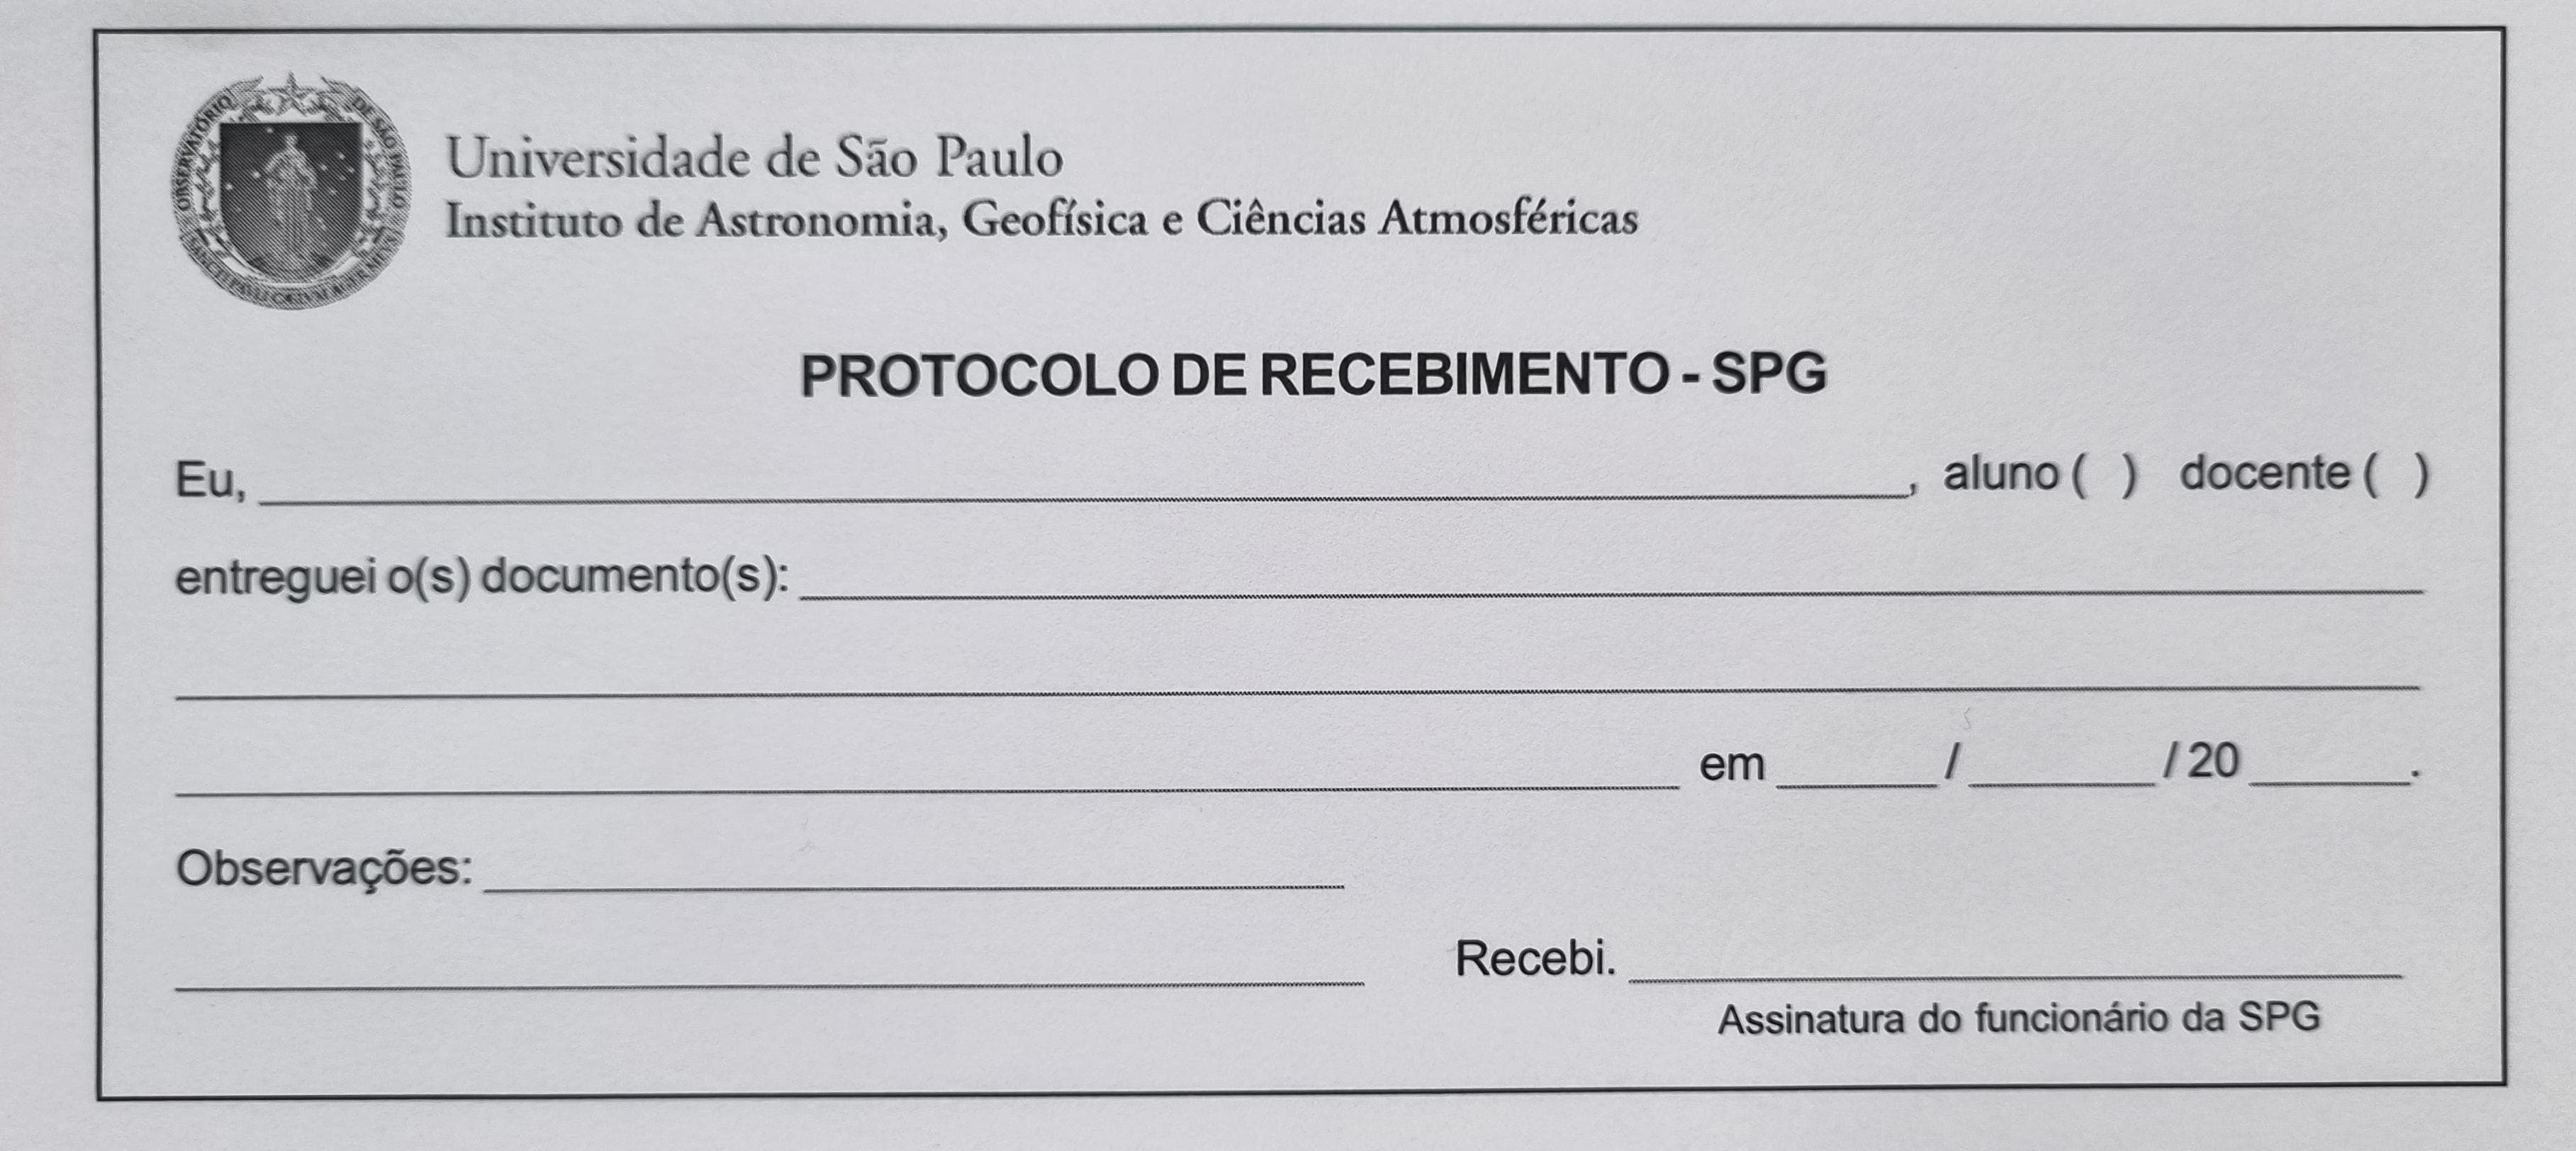
\includegraphics[width=\linewidth]{protocolo_recebimento.jpeg}
      \caption{Foto do protocolo de recebimento de depósito, que você precisa escanear e colocar no Janus.}
      \label{fig:protocolo}
    \end{figure}

    Para imprimir a tese, você pode aproveitar a parceria que o IAG tem com a gráfica do IME. Você só precisa mandar um email para a CCP (\url{ccpastro iag.usp.br}) pedindo autorização. Quando ela for dada, é só encaminhar o email para a Cida (\url{cida.coelho@iag.usp.br}), que fará a solicitação junto à grafica. Quando a impressão estiver pronta, depois de um ou dois dias, ela irá te avisar para você poder fazer a retirada. Note que talvez você tenha que falar com outra pessoa ao invés da Cida quando fizer a solicitação (este texto foi escrito em 2024).

    Tanto o formulário de sugestão da banca quanto a carta de manifestação do orientador estão disponíveis na seção de formulários do site do IAG (\url{https://www.iag.usp.br/pos-graduacao/formularios}), na parte ``8 - Defesa de Dissertações e Teses''. Para a sugestão da banca, a maioria dos examinadores deverá ser de fora do programa e pelo menos um de fora do IAG. Para o mestrado são necessários três titulares e três suplentes, enquanto que no doutorado são 5 titulares e 5 suplentes. Em ambos os casos você precisa colocar o nome do seu orientador(a) e um suplente correspondente. Recomendo você começar a conversar sobre os nomes um mês antes da data que você deseja fazer o depósito, assim você pode enviar emails para os examinadores perguntando se aceitam compor sua banca.

    Depois de entregar os documentos, a CCP irá julgar a sugestão para a banca e, caso aprovada, você terá até 105 dias para realizar a defesa. Caso queira defender em menos de 30 dias, é necessário preencher um termo de responsabilidade (também presente na parte de formulários do site do IAG).

  \section{Características deste template}
    Este template foi criado tendo como base o repositório Web\LaTeX{}, que por sua vez foi criado para substituir o Overleaf. A vantagem neste caso é a integração com o GitHub, permitindo o controle de versões, por exemplo, o uso de Codespaces (que são computadores virtuais, criados através do GitHub) caso você queira, e a possibilidade de usar extensões como Grammarly, LTex e Copilot. Caso você não queira usar um Codespace (pois ele é limitado a 180 horas de uso por mês), você também pode clonar o repositório pra o seu PC e trabalhar normalmente. Isso é possível pois o WebLaTex define um container com toda a informação necessária para você compilar seus documentos.

    \subsection{Web\LaTeX{}}
      O WebLaTex foi criado como uma alternativa de acesso aberto ao Overleaf, quando este começou a cobrar pelo serviço. Ele usa o VSCode como base e traz algumas extensões por padrão, como o GitHub Copilot, Grammarly, \LaTeX{} Workshop. Também existem algumas opcionais, como a Live Share, que permite que várias pessoas escrevam no mesmo arquivo simultaneamente (similar ao Overleaf).

      Da forma que ele está configurado neste template, o \LaTeX{} irá compilar o seu arquivo toda vez que você salvar, respeitando um intervalo mínimo de 15 segundos entre compilações. Você pode mudar isso nas opções, digitando ``auto build'' na busca e mudando os valores do ``Auto Build: Interval'' e do ``Auto Build: Run''.

      Você pode encontrar mais detalhes sobre Web\LaTeX{} no site do repositório: \url{https://github.com/sanjib-sen/WebLaTex}.

    \subsection{VSCode e suas extensões}
      Usando estes templates, você pode escrever seu texto usando o VSCode (ou o VSCodium). Este editor possui diversas opções de customização, desde a aparência até suas extensões.

      Na presente versão, o template habilita, além das extensões do WebLaTex, a extensão ``GitDoc''. Esta extensão faz commit+push automaticamente toda vez que você salva o arquivo ou em intervalos definidos pelo usuário. Você pode mudar as configurações do GitDoc indo nas opções e escrevendo ``gitdoc'' na busca. Por padrão, ele faz os commits e pushs a cada 30 segundos, caso existam mudanças.

    \subsection{Acrônimos}
      Para facilitar o gerenciamento de acrônimos, este template usa o pacote \ttt{acro}. Os acrônimos devem ser definidos previamente no arquivo ``Sections/0.2-list\_of\_acronyms.tex'', usando o seguinte formato:
      %
      \begin{lstlisting}[autogobble]
        \DeclareAcronym{acronym}{
          short = short name,
          long  = long name,
          cite  = citation %optional
        }
      \end{lstlisting}

      Desta forma, a primeira referência à um acrônimo é escrita normalmente, usando a forma ``longa'' e citando a referência, caso você tenha a definido. Por exemplo, o comando \ttt{\textbackslash ac\{splus\}} resultará em \ac{splus}.

      Se o acrônimo é usado apenas uma vez, como no caso anterior, ele não exibe a versão curta do nome. Caso você queira forçar que isso aconteça, mesmo que só use o acrônimo uma única vez, é só combinar o comando \ttt{\textbackslash ac\{vhs\}} com o \ttt{\textbackslash acuse\{vhs\}}. Por exemplo: \ac{vhs}\acuse{vhs}.

      Você também pode incluir texto usando o math-mode (\ttt{\textbackslash ac\{photoz\}}) \ac{photoz}. Você também pode usar o acrônimo no plural (\ttt{\textbackslash acp\{photoz\}}) \acp{photoz}, forçar o modo curto (\ttt{\textbackslash acs\{specz\}}) \acs{specz} ou longo (\ttt{\textbackslash acl\{specz\}}) \acl{specz}. Há também a possibilidade de colocar a primeira letra em maiúsculo (\ttt{\textbackslash Ac\{specz\}}) \Ac{specz}.

    \subsection{Citações}
      As citações são gerenciadas com o pacote \ttt{natbib}, e definidas no arquivo ``Sections/6-bibliography.tex'', no qual a lista com referências usadas é importada do arquivo ``Sections/reference\_list.bib''. 

      Este pacote suporta diferentes tipos de citações, todas descritas em detalhes aqui: \url{https://gking.harvard.edu/files/natnotes2.pdf}.

      Uma dica adicional para deixar o seu arquivo de referências bem organizado e bonito é usar o Bibtex Tidy (\url{https://flamingtempura.github.io/bibtex-tidy/index.html}), que alinha, ordena e arruma as citações.

    \subsection{Exemplos}
      Colocarei aqui alguns exemplos de imagens, tabelas, listings, equações e etc para facilitar a escrita do seu trabalho.

      \subsubsection{Imagens}
      Uma imagem centralizada no texto (Figura \ref{fig:ex_1col}):
      %
      \begin{figure}[h]
        \centering
        \includegraphics[width=0.5\linewidth]{example-image-a}
        \caption{Exemplo de imagem em uma coluna.}
        \label{fig:ex_1col}
      \end{figure}

      Duas imagens centralizadas no texto (Figura \ref{fig:sub_1} e \ref{fig:sub_2}, partes da Figura \ref{fig:ex_2cols}). Você pode fazer como neste exemplo, mas eu recomendo que faça isso direto no \ttt{Python} e coloque no \LaTeX{} como uma imagem só:
      %
      \begin{figure}[h]
        \centering
        \begin{subfigure}{.45\textwidth}
          \centering
          \includegraphics[width=0.8\linewidth]{example-image-a}
          \caption{Subfigura 1}
          \label{fig:sub_1}
        \end{subfigure}%
        \begin{subfigure}{.45\textwidth}
          \centering
          \includegraphics[width=0.8\linewidth]{example-image-b}
          \caption{Subfigura 2}
          \label{fig:sub_2}
        \end{subfigure}
        \caption{Uma imagem contendo duas subfiguras}
        \label{fig:ex_2cols}
      \end{figure}

      Para não numerar as figuras, é só colocar um asterisco no final do nome do ambiente (figure $\rightarrow$ figure*).
      
      \subsubsection{Tabelas}
        Este template usa o pacote \ttt{booktabs}, que permite fazer tabelas mais bonitas. Repare no uso do ``toprule'', ``midrule'', e ``bottomrule'':
        %
        \begin{table}[h!]
          \centering
          \caption{Exemplo de tabela.}
          \label{tab:ex_1}
          \begin{tabular}{ccc}
            \toprule
            \textbf{Coluna 1} & \textbf{Coluna 2} & \textbf{Coluna 3} \\ \midrule
            Célula 1          & Célula 2          & Célula 3          \\ 
            Célula 4          & Célula 5          & Célula 6          \\ 
            \bottomrule
          \end{tabular}
        \end{table}

        Caso queira tirar as ``sobras'' à esquerda e à direita, é só incluir um ``@\{\}'' antes e depois da configuração das colunas:
        %
        \begin{table}[h!]
          \centering
          \caption{Exemplo de tabela sem as margens.}
          \label{tab:ex_2}
          \begin{tabular}{@{}ccc@{}}
            \toprule
            \textbf{Coluna 1} & \textbf{Coluna 2} & \textbf{Coluna 3} \\ \midrule
            Célula 1          & Célula 2          & Célula 3          \\ 
            Célula 4          & Célula 5          & Célula 6          \\ 
            \bottomrule
          \end{tabular}
        \end{table}

        Outras opções para as colunas são \ttt{c} para centralizado, \ttt{l} para alinhado à esquerda, \ttt{r} para alinhado à direita, e \ttt{p\{X\}} para ter uma célula com tamanho fixo X (que pode ser dado em cm):
        %
        \begin{table}[h!]
          \centering
          \caption{Exemplo de tabela com tamanho fixo.}
          \label{tab:ex_3}
          \begin{tabular}{@{}lrp{5cm}@{}}
            \toprule
            \textbf{Coluna 1} & \textbf{Coluna 2} & \textbf{Coluna 3} \\ \midrule
            Célula 1          & Célula 2          & Célula 3          \\ 
            Célula 4          & Célula 5          & Célula 6          \\ 
            \bottomrule
          \end{tabular}
        \end{table}

        Você também pode criar células que abrangem várias linhas ou colunas usando os comandos \ttt{\textbackslash multirow\{número de linhas\}\{tamanho (ou * para automático)\}\{Texto\}} e \ttt{\textbackslash multicolumn\{número de colunas\}\{alinhamento (l, r, caption)\}\{Texto\}}:
        %
        \begin{table}[h!]
          \centering
          \caption{Exemplo de tabela com multirows e multicolumns.}
          \label{tab:ex_4}
          \begin{tabular}{@{}ccc@{}}
            \toprule
            \textbf{Coluna 1}             & \textbf{Coluna 2} & \textbf{Coluna 3} \\ \midrule
            \multirow{2}{*}{Célula 1 e 4} & \multicolumn{2}{c}{Células 2 e 3}     \\ 
                                          & Célula 5          & Célula 6          \\ 
            \bottomrule
          \end{tabular}
        \end{table}

        O template também inclui o pacote \ttt{threeparttable}, que permite colocar notas de rodapé em tabelas:
        %
        \begin{table}[h!]
          \centering
          \caption{Exemplo de tabela usando o \ttt{threeparttable}.}
          \label{tab:ex_5}
          \begin{threeparttable}
            \begin{tabular}{ccc}
              \toprule
              \textbf{Coluna 1} & \textbf{Coluna 2} & \textbf{Coluna 3} \\ \midrule
              Célula 1\tnote{a} & Célula 2          & Célula 3\tnote{c} \\ 
              Célula 4          & Célula 5\tnote{b} & Célula 6          \\ 
              \bottomrule
            \end{tabular}
            \begin{tablenotes}
              \item[a] Célula 1.
              \item[b] Célula 5.
              \item[c] Célula 3.
            \end{tablenotes}
          \end{threeparttable}
        \end{table}

        Para não numerar as tabelas, é só colocar um asterisco no final do nome do ambiente (table $\rightarrow$ table*).

      \subsubsection{Listings (códigos)}
        Para colocar códigos no texto, este template usa o pacote \ttt{listings} que, apesar de não ser tão completo quanto o \ttt{minted}, não usa o \ttt{Python} como requisito. Um exemplo de código geral foi dado acima, na forma de definir acrônimos:
        %
        \begin{lstlisting}[autogobble]
          \DeclareAcronym{acronym}{
            short = short name,
            long  = long name,
            cite  = citation %optional
          }
        \end{lstlisting}

        Porém você pode definir estilos (configurados no arquivo ``Sections/0.1-configurations.tex''). O estilo para Python já está definido (Código \ref{code}):
        %
        \begin{lstlisting}[label=code, language=Python, numbers=left, autogobble]
          class Nome():
          """
          Exemplo de classe para o template
      
          Args:
            ...
      
          Attributes:
            ...
      
          Methods:
            ...
      
          Returns:
            ...
          """
      
          def __init__(self, in_features, out_features):
              super().__init__()
              self.in_features = in_features
              self.out_features = out_features

          ...
        \end{lstlisting}

        Nos dois casos, o parâmetro ``autogobble'' serve para tirar espaços em branco extras. Não há como deixar o código sem numeração.

      \subsubsection{Equações}
        Equação simples, como a Equação \eqref{eq:drake}:
        %
        \begin{equation}
          N = R_* \cdot f_\text{P} \cdot n_e \cdot f_\text{l} \cdot f_\text{i} \cdot f_\text{c} \cdot L
          \label{eq:drake}
        \end{equation}

        Também é possível criar equações de várias linhas, com alinhamento (Equação \eqref{eq:aligned}):
        %
        \begin{align}
          y &= a \cdot x + b, \\
          k &= a \cdot x^2 + b \cdot x + c
          \label{eq:aligned}
        \end{align}

        E, por último, criar ``cases'' (Equação \eqref{eq:cases}). Só é necessário quebrar a linha dentro do ambiente \ttt{cases}:
        %
        \begin{align}
          x =
          \begin{cases}
            y,\text{ se } a > 0 \\
            z,\text{ se } a \leq 0
          \end{cases}
          \label{eq:cases}
        \end{align}

        Para não numerar as equações, é só colocar um asterisco no final do nome do ambiente (equation ou align $\rightarrow$ equation* ou align*).

      \subsection{Fazendo plots no \ttt{Matplotlib}}
        Para facilitar a vida, existe uma função que permite que você faça plots no \ttt{Matplotlib} com as dimensões exatas para colocar no seu texto, sem precisar mexer com as opções do \ttt{\textbackslash includegraphics}. A função é descrita em \url{https://jwalton.info/Embed-Publication-Matplotlib-Latex/}, e a função é:
        %
        \begin{lstlisting}[label=code, language=Python, numbers=left, autogobble]          
          def set_size(width, fraction=1, subplots=(1, 1)):
              """Set figure dimensions to avoid scaling in LaTeX.
          
              Parameters
              ----------
              width: float or string
                      Document width in points, or string of predined document type
              fraction: float, optional
                      Fraction of the width which you wish the figure to occupy
              subplots: array-like, optional
                      The number of rows and columns of subplots.
              Returns
              -------
              fig_dim: tuple
                      Dimensions of figure in inches
              """
              if width == 'thesis':
                  width_pt = 426.79135
              elif width == 'beamer':
                  width_pt = 307.28987
              else:
                  width_pt = width
          
              # Width of figure (in pts)
              fig_width_pt = width_pt * fraction
              # Convert from pt to inches
              inches_per_pt = 1 / 72.27
          
              # Golden ratio to set aesthetic figure height
              # https://disq.us/p/2940ij3
              golden_ratio = (5**.5 - 1) / 2
          
              # Figure width in inches
              fig_width_in = fig_width_pt * inches_per_pt
              # Figure height in inches
              fig_height_in = fig_width_in * golden_ratio * (subplots[0] / subplots[1])
          
              return (fig_width_in, fig_height_in)
        \end{lstlisting}

        Junto com essa definição, você deve configurar o \ttt{Matplotlib} pra usar estas configurações:
        %
        \begin{lstlisting}[label=code, language=Python, numbers=left, autogobble]          
          # Plot visual settings
          thesis_settings = {
              # Use LaTeX to write all text
              "text.usetex": False,
              "font.family": "serif",
              # Use 10pt font in plots, to match 10pt font in document
              "font.size": 10,
              "axes.labelsize": "medium",
              "axes.titlesize": "medium",
              "figure.labelsize": "medium",
              "figure.titlesize": "medium",
              # Make the legend/label fonts a little smaller
              "legend.fontsize": "small",
              "legend.title_fontsize": "small",
              "xtick.labelsize": "small",
              "ytick.labelsize": "small",
              # Enable axis grids
              "axes.grid": True,
              "grid.alpha": 0.5,
          }

          plt.rcParams.update(thesis_settings)
        \end{lstlisting}

        Feito isso, quando você for criar uma figura nova, é só chamar a função no argumento \ttt{figsize} usando \ttt{width = 455.24411} (que é a largura deste documento em pt). Por exemplo:
        \begin{lstlisting}[label=code, language=Python, numbers=left, autogobble]          
          fig, axes = plt.subplots(1, 2, figsize=set_size(width, suplots=(1, 2), fraction=1))
          ...
        \end{lstlisting}

        As outras opções e mais detalhes deste código estão descritas no link acima. Dois exemplos de imagens geradas com essa função estão nas Figuras \ref{fig:matplot_1} e \ref{fig:matplot_2}.
        %
        \begin{figure}[h]
          \centering
          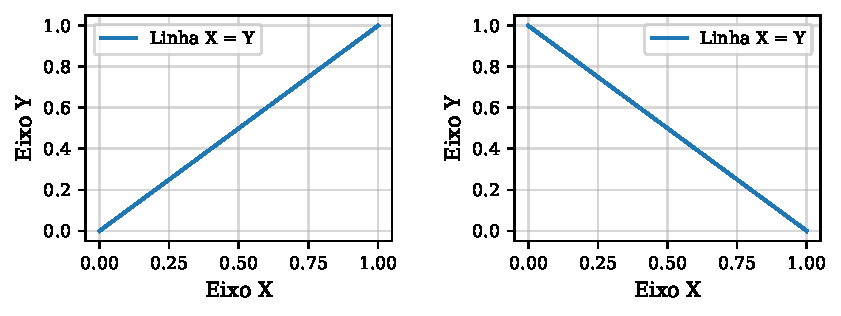
\includegraphics{exemplo_matplot_2.pdf}
          \caption{Exemplo de figura feita usando a função \ttt{set\_size}.}
          \label{fig:matplot_1}
        \end{figure}
        %
        \begin{figure}[h]
          \centering
          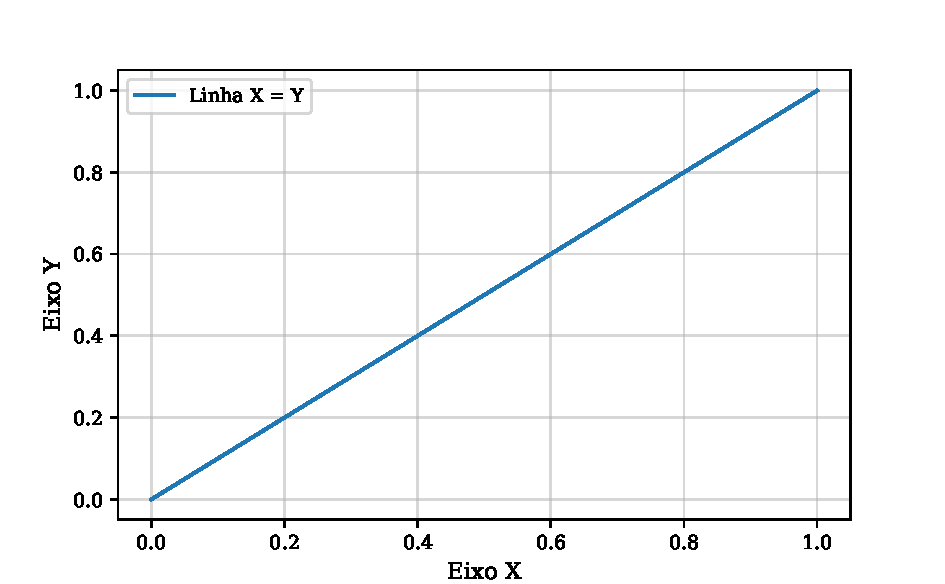
\includegraphics{exemplo_matplot.pdf}
          \caption{Exemplo de figura feita usando a função \ttt{set\_size}.}
          \label{fig:matplot_2}
        \end{figure}

        Note que nenhum caractere dentro da imagem tem tamanho menor do que os da legenda (que é um bom teste para saber se o tamanho das letras e números está bom) e como a imagem ocupa quase toda a largura do texto mesmo sem ser necessário usar a opção [width=\textbackslash linewidth].

      %     In this template, the citations are handled by the \ttt{natbib} package, with is defined by the commands in the ``Sections/6-bibliography.tex'' file. There, the list of used references are imported from the ``Sections/reference\_list.bib'' file.

  %     This package supports different types of citations, all of them explained here: \url{https://gking.harvard.edu/files/natnotes2.pdf}


  % The goal of this document is to provide an unofficial dissertation/thesis template for IAG/USP.

  % \section{General tips for when writing a dissertation/thesis}

  % When writing the text, you should be aware of the IAG/USP norms\footnote{\url{https://leginf.usp.br/?resolucao=resolucao-copgr-no-7882-de-25-de-novembro-de-2019}}. There are some obligatory chapters that should be in the text, the list is shown in ``XI – PROCEDIMENTOS PARA DEPÓSITO DA DISSERTAÇÃO/TESE''.

  % In order to make the deposit, you should have:
  % %
  % \begin{itemize}
  %   \item For PhD: a printed copy of the text, the forms containing the committee suggestion, a letter from the supervisor saying that you are fit for the defense, and proof of one published paper, where you are the first or second co-author, in a refereed international journal. You also need to make a deposit in Janus.
  %   \item For master's: 
  % \end{itemize}

  % IAG has a partnership with the IME's print shop. To print your dissertation/thesis with them you should send an email to \url{ccpastro iag.usp.br} with copy to \url{cida.coelho@iag.usp.br} asking for permission, with the PDF of the text attached. If approved, the text will be sent to the print shop and you will be notified when it is ready (within 1 or 2 days).

  % The forms for the committee and the supervisor manifestation can be found at IAG's website, in the ``Forms'' page: \url{https://www.iag.usp.br/pos-graduacao/formularios}. I recommend that you start thinking about the names that should be in your defense two weeks before making the deposit, and sending each member an email one week before, asking if they accept that their names be suggested.

  % \section{Features of this template}

  %   This template is based on the \ttt{WebLatex}\footnote{\url{https://github.com/sanjib-sen/WebLaTex}} template, created to replace Overleaf with Github, with some modifications. See the link for further details and the advantages of this approach.

  %   We also included the GitDoc extension, which automatically makes commit+push to a repository. To use it, you should enable the extension using \ttt{ctrl+shift+p} > ``GitDoc Enable''
  
  %   \subsection{Acronyms}
  %     The acronyms in this model are handled by the \ttt{acro} package, where you need to defined the acronyms beforehand, in the ``Sections/0.2-list\_of\_acronyms.tex'', using the format:

  %     \begin{lstlisting}[autogobble]
  %       \DeclareAcronym{acronym}{
  %         short = short name,
  %         long  = long name,
  %         cite  = citation %optional
  %       }
  %   \end{lstlisting}

  %   Using this package, the first reference to an acronym is written normally, with the reference if you defined the acronym with one, using the ``long'' name: \ac{splus}. Whenever you make another reference to this acronym, it will use the ``short'' name: \ac{splus}.
    
  %   You can also define acronyms using math-mode: \ac{photoz}. If you use the acronym only once, it will be printed using the long form only, without diplaying the short form, in this case, use can use the \ttt{\textbackslash ac\{acro\}} command followed by  \ttt{\textbackslash acuse\{acro\}}: \ac{specz}\acuse{specz}.

  %   There are some variations on how the acronyms can be printed, such as:
  %   \begin{itemize}
  %     \item Plural: \ttt{\textbackslash acp\{photoz\}} $\rightarrow$ \acp{photoz}
  %     \item Force long name: \ttt{\textbackslash acl\{des\}} $\rightarrow$ \acl{des}
  %     \item Force short name: \ttt{\textbackslash acs\{vhs\}} $\rightarrow$ \acs{vhs}
  %     \item Capital first letter: \ttt{\textbackslash Ac\{photoz\}} $\rightarrow$ \Ac{photoz}
  %   \end{itemize}

  %   \subsection{Citations}
  %     In this template, the citations are handled by the \ttt{natbib} package, with is defined by the commands in the ``Sections/6-bibliography.tex'' file. There, the list of used references are imported from the ``Sections/reference\_list.bib'' file.

  %     This package supports different types of citations, all of them explained here: \url{https://gking.harvard.edu/files/natnotes2.pdf}

  %   \subsection{Examples of tables, figures, listings...}

  %   \subsection{Making figures with \ttt{Matplotlib}}
\chapter{\chapternamedatabase}\label{cap:database}

Neste capítulo, apresentamos os dados utilizados neste trabalho, incluindo as fontes de dados fotométricos. Os dados espectroscópicos serão apresentados e discutidos no apêndice \ref{chap:spectra} e no capítulo \ref{chap:spectra_emission}. 

Primeiramente, descrevemos o levantamento \ac{splus}, suas características e os dados obtidos. Em seguida, detalhamos os procedimentos de correção de extinção aplicados às magnitudes fotométricas. Apresentamos também como os dados foram selecionados para a análise, incluindo os parâmetros utilizados para a fotometria e a seleção de galáxias, magnitudes limites e flags de qualidade.

\section{S-PLUS}
O \ac{splus}, um levantamento do céu do hemisfério sul, localizado no Cerro Tololo Inter-American Observatory, Chile (CTIO), tem como objetivo observar uma área de 9300 graus quadrados do céu com o telescópio robótico de 80 cm T80-South \citep{oliveira2019splus}. Ele disponibiliza 12 filtros fotométricos (Figura \ref{splus_filters}), sendo 5 de banda larga ($u$, $g$, $r$, $z$) e 7 de banda estreita (J0378, J0395, J0410, J0430, J0515, J0660 e J0861).

\begin{figure}[!ht]
    \begin{center}
    % \setcaptionmargin{1cm}
    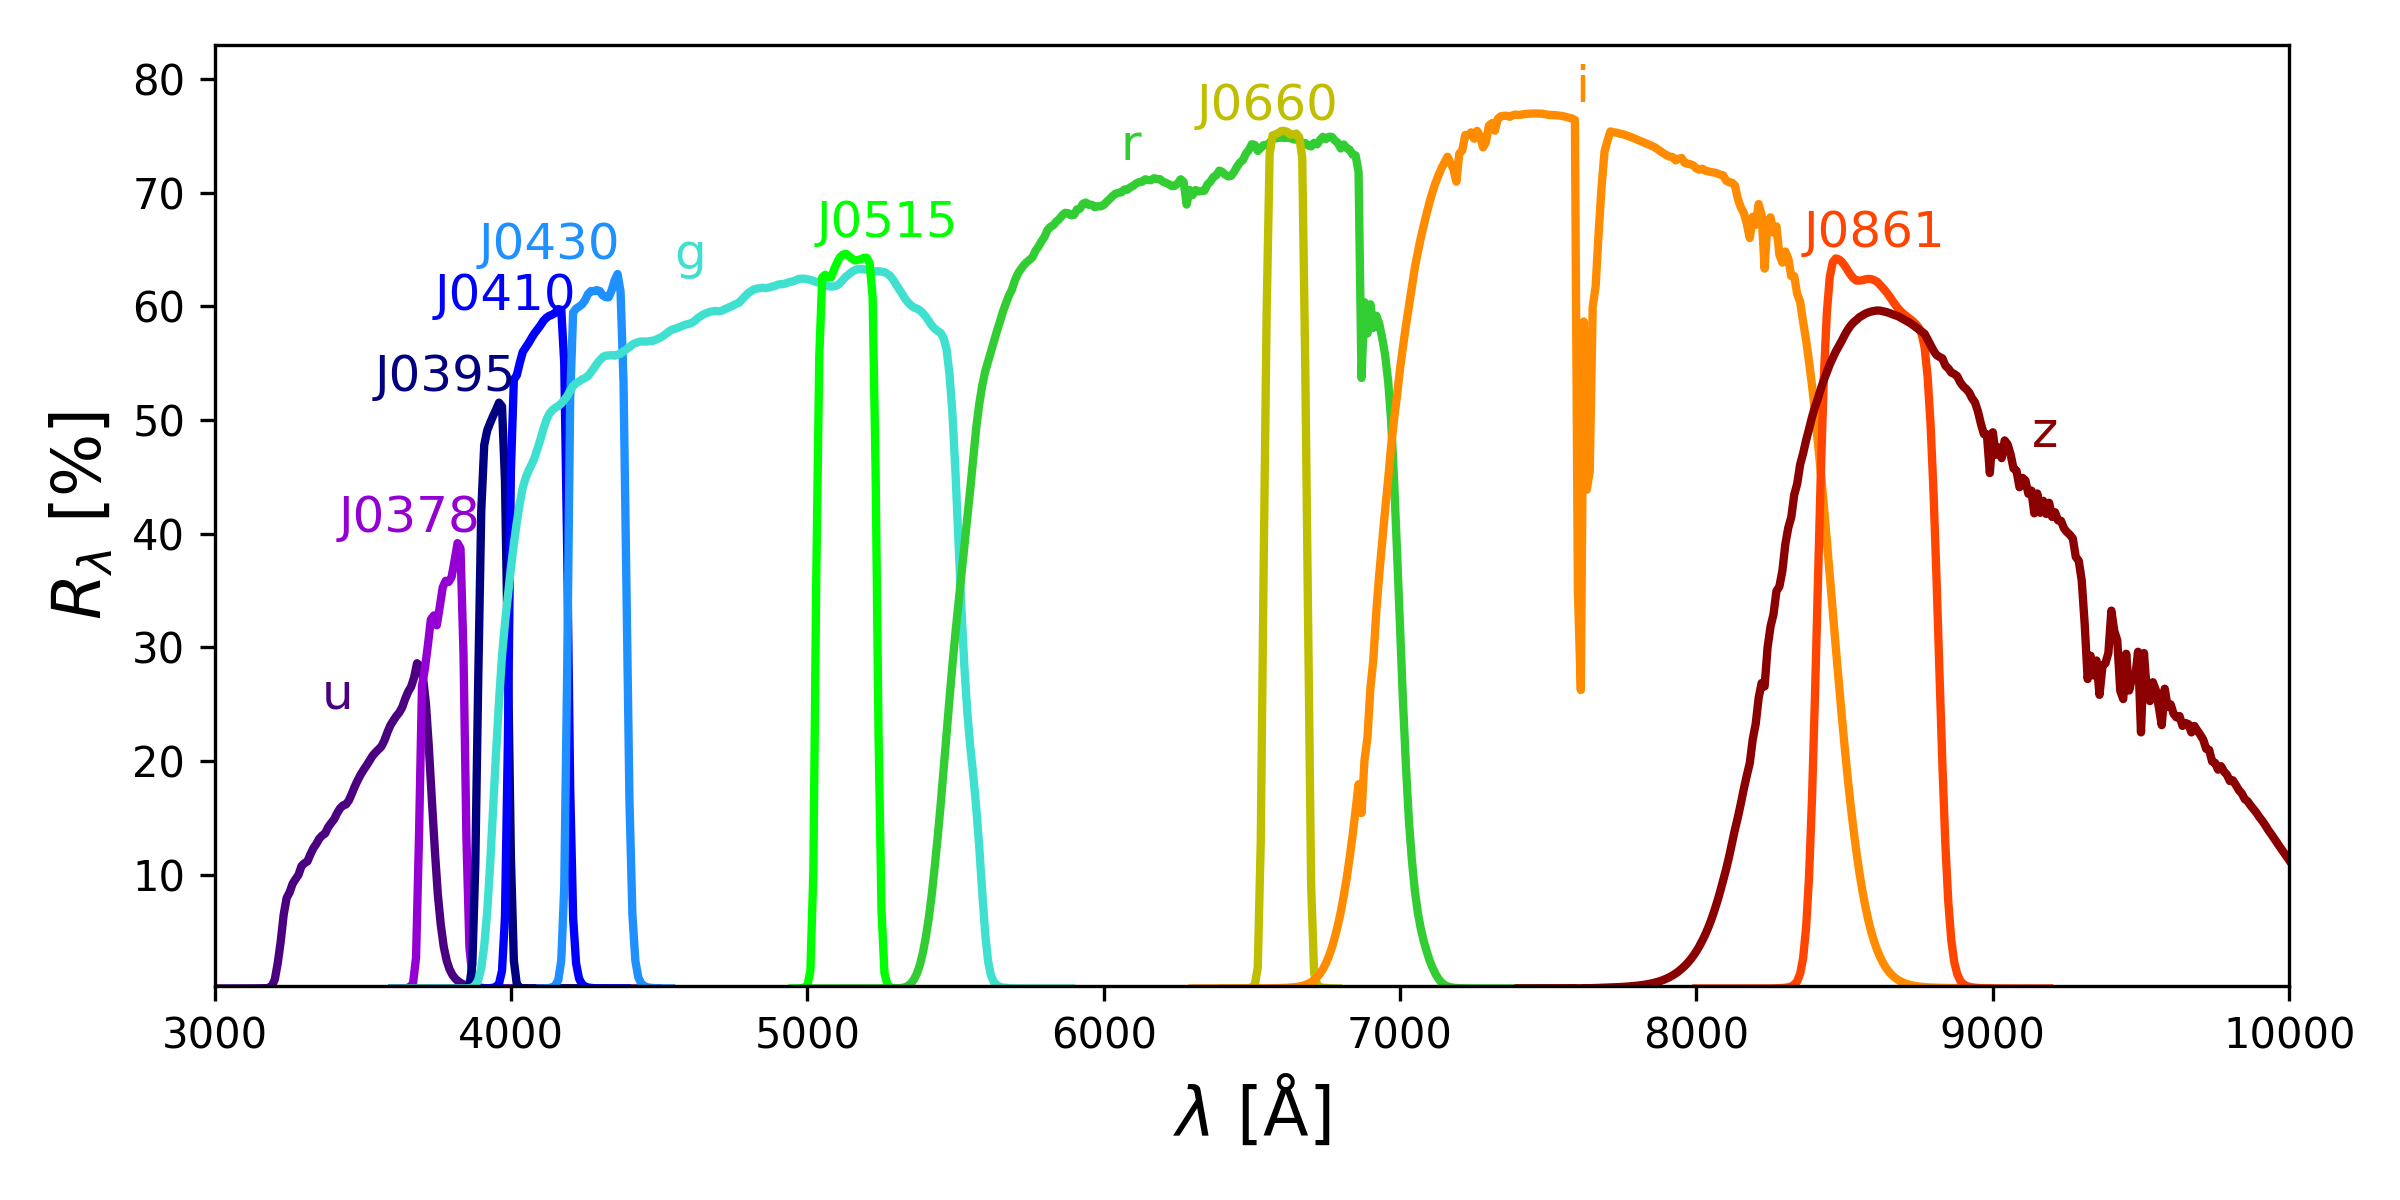
\includegraphics[width=1.0 \columnwidth,angle=0]{splus_filters.png}
    \caption[]{Curvas de resposta dos 12 filtros fotométricos do S-PLUS \citep{splus_DR4_footprint}.}
    \label{splus_filters}
    \end{center}
\end{figure}

Os dados utilizados neste trabalho foram obtidos a partir do quarto lançamento de dados do S-PLUS (\ac{DR4}) \citep{herpich2024fourthsplusdatarelease}. O DR4 cobre uma área de 3022,7 graus quadrados, composta por 1629 campos, cada um deles com um campo de visão de aproximadamente 2 graus quadrados. A Figura \ref{footprint_iDR4} mostra a área coberta pelo S-PLUS \ac{DR4}.

\begin{figure}[!ht]
    \begin{center}
    % \setcaptionmargin{1cm}
    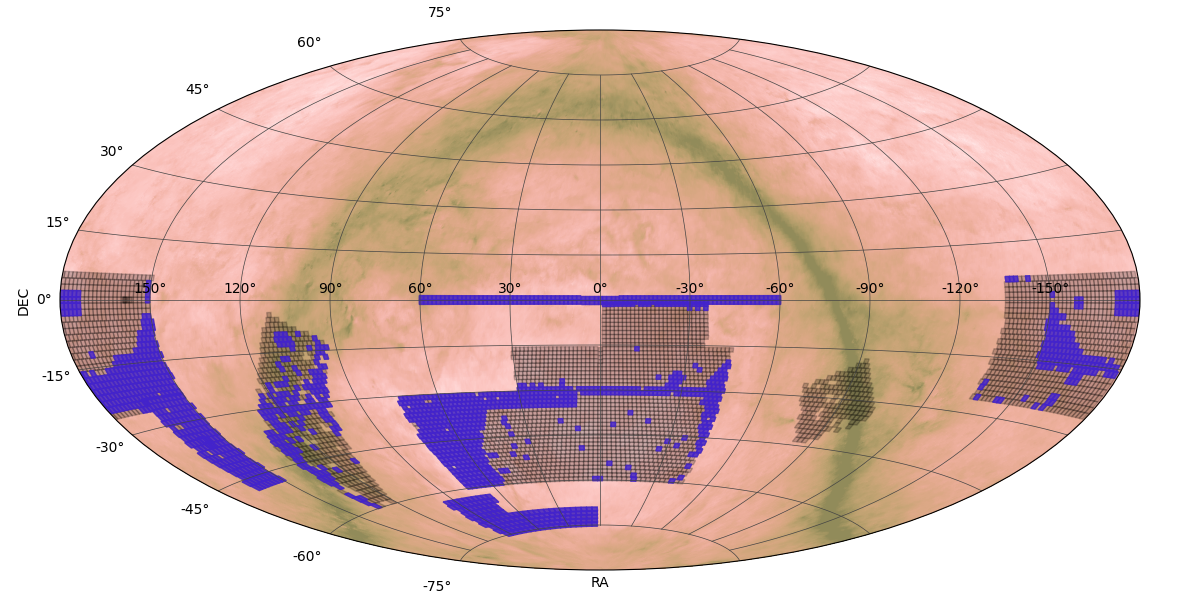
\includegraphics[width=1.0 \columnwidth,angle=0]{footprint_iDR4.png}
    \caption[]{Área coberta pelo S-PLUS DR4. Campos em azul são os observados até o DR4.}
    \label{footprint_iDR4}
    \end{center}
\end{figure}

Além dos 12 filtros fotométricos mencionados, temos opções dos tipos de magnitudes para cada uma dessas bandas. Entre os tipos de magnitudes disponíveis, destacam-se:

\begin{itemize}
    \item \textbf{ISO}: Captura o fluxo dentro de uma isofota, definida por um limite de brilho superficial constante.
    \item \textbf{PETRO}: Mede o fluxo utilizando a abertura de Petrosian, que captura uma fração constante da luz total da galáxia, minimizando a perda de luz nas regiões externas.
    \item \textbf{AUTO}: Abertura adaptativa que utiliza um algoritmo automático para ajustar a abertura ao tamanho e forma do objeto.
    \item \textbf{APER\_3}: Abertura fixa de 3 pixels de raio, adequada para medir o fluxo em regiões centrais.
    \item \textbf{APER\_6}: Abertura fixa de 6 pixels de raio, usada para capturar uma área maior do objeto, balanceando entre evitar contaminação de fontes próximas e capturar mais do fluxo total.
\end{itemize}

Para este trabalho, escolhemos utilizar as magnitudes baseadas na abertura APER\_6. A escolha foi motivada pela necessidade de uma medida consistente para os objetos mais compactos, como as galáxias ultracompactas (UCDs) que estamos buscando.


\subsection{Fotometria de Fornax}\label{sec:Fornax_data}
Os dados do aglomerado de Fornax foram obtidos a partir da mesma fonte que os dados do S-PLUS, o DR4. Porém, a partir da colaboração descrita em \cite{castelli2024splusfornaxprojectsfp}, utilizamos a fotometria de \cite{haack2024splusfornaxprojectsfp}, onde foram realizadas novas execuções específicas do \ac{SExtractor} (SExtractor) no DR4, identificando o conjunto mais adequado de parâmetros para recuperar o máximo possível de galáxias de Fornax com fotometria confiável e evitando duplicações.

Os parâmetros da RUN 1 de \cite{haack2024splusfornaxprojectsfp} foram projetados para identificar galáxias fracas e objetos compactos próximos a galáxias mais brilhantes. Por outro lado, os parâmetros da RUN 2 são voltados para uma boa caracterização de galáxias brilhantes e extensas. Assim, para detectar objetos compactos como anãs ultra-compactas (UCDs) ou aglomerados globulares (GCs) perto das galáxias de Fornax, os parâmetros da RUN 1 são mais adequados. Já para caracterizar melhor os objetos mais brilhantes e extensos em Fornax, os parâmetros da RUN 2 são mais eficazes. No nosso caso, usamos os dados da RUN 1. Assim, todos as magnitudes e parâmetros dos \ac{SExtractor} que usamos ao longo do trabalho são da RUN 1 de \cite{haack2024splusfornaxprojectsfp}.


\subsection{Correção da extinção}\label{sec:Coeficientes_ext}

As magnitudes utilizadas não estão corrigidas para a extinção interestelar. A poeira galáctica pode afetar significativamente as medições fotométricas, especialmente em áreas do céu com alta densidade de poeira. Para preparar os dados fotométricos para a análise, é necessário aplicar uma correção de extinção.

Através do pacote Python \texttt{dustmaps} \citep{dustmapsGreen2018}, utilizamos o mapa de poeira CSFD \citep{chiang2023correctedsfdaccurategalactic}. O mapa CSFD é uma versão melhorada do mapa de Schlegel-Finkbeiner-Davis (SFD) (\citealt{Schlegel_1998} \& \citealt{Schlafly_2011}), que é comumente utilizado para estimar a extinção em diferentes direções do céu. A correção fornecida pelo CSFD ajuda a reduzir os efeitos da estrutura em larga escala e da contaminação do fundo infravermelho cósmico (CIB). Com esses efeitos removidos, o mapa CSFD fornece um valor mais preciso e confiável da extinção interestelar.

\textbf{Cálculo dos Coeficientes de Extinção}

Para converter as estimativas de extinção fornecidas pelo mapa de poeira em correções aplicáveis às magnitudes fotométricas, utilizamos a lei de extinção de \cite{cardelli1989dust}. Para cada uma das 12 magnitudes, calculamos os coeficientes de extinção com base nos comprimentos de onda efetivos das respectivas bandas.

\sloppy
O cálculo dos coeficientes de extinção foi realizado utilizando o pacote Python \texttt{extinction} de \cite{barbary2017extinction}, que implementa a lei de \cite{cardelli1989dust} e permite a aplicação direta das correções de extinção às magnitudes observadas.

\subsection{Cortes de qualidade na fotometria}\label{subsec:cuts}
Para garantir a qualidade dos dados fotométricos utilizados neste trabalho, aplicamos uma série de cortes de qualidade nas magnitudes. Esses cortes foram definidos com base em parâmetros específicos fornecidos pelo S-PLUS DR4 dos dados de Fornax, utilizando os parâmetros da RUN 1 de \cite{haack2024splusfornaxprojectsfp}.

Descartamos, nas 12 magnitudes da abertura APER\_6, magnitudes maiores do que 30, evitando objetos com baixa qualidade de medição e com erros fotométricos altos. Descartamos também em cada uma das mesmas bandas valores de \textit{flag0}$\leq$3, que são objetos com problemas de qualidade de medição.

Na seleção dos objetos utilizados nas próximas seções para a busca de galáxias ultracompactas, adotamos a banda \textit{g\_APER\_6} como referência principal. Aplicamos um corte inferior em \textit{g\_APER\_6}=13 para excluir objetos muito brilhantes e saturados, garantindo a qualidade das medições. Além disso, estabelecemos um corte superior em \textit{g\_APER\_6}=21, visando minimizar a contaminação por aglomerados globulares. Esses critérios de seleção seguem \cite{Cantiello_2020}, que adotam um critério de separação de GCs de UCDs com $M_g=-10.5$, que corresponde a $M_v\sim -11$ mag ($\sim10^7 M_\odot$) e uma magnitude aparente de $m_g=21$. O módulo de distância adotado para Fornax é de $m-M=31.5$, apresentado na Tabela \ref{tab:properties_fornax}.

Dos dados do S-PLUS DR4, temos um total de 2900926 objetos. Após a aplicação dos cortes de qualidade, restaram 619630 objetos.

Das 12 magnitudes utilizadas no S-PLUS na abertura APER\_6 corrigidas, com os cortes descritos anteriormente, apresentamos na Figura \ref{fig:hist_distri_mags_data} as distribuições resultantes.

\begin{figure}[!ht]
    \begin{center}
    % \setcaptionmargin{1cm}
    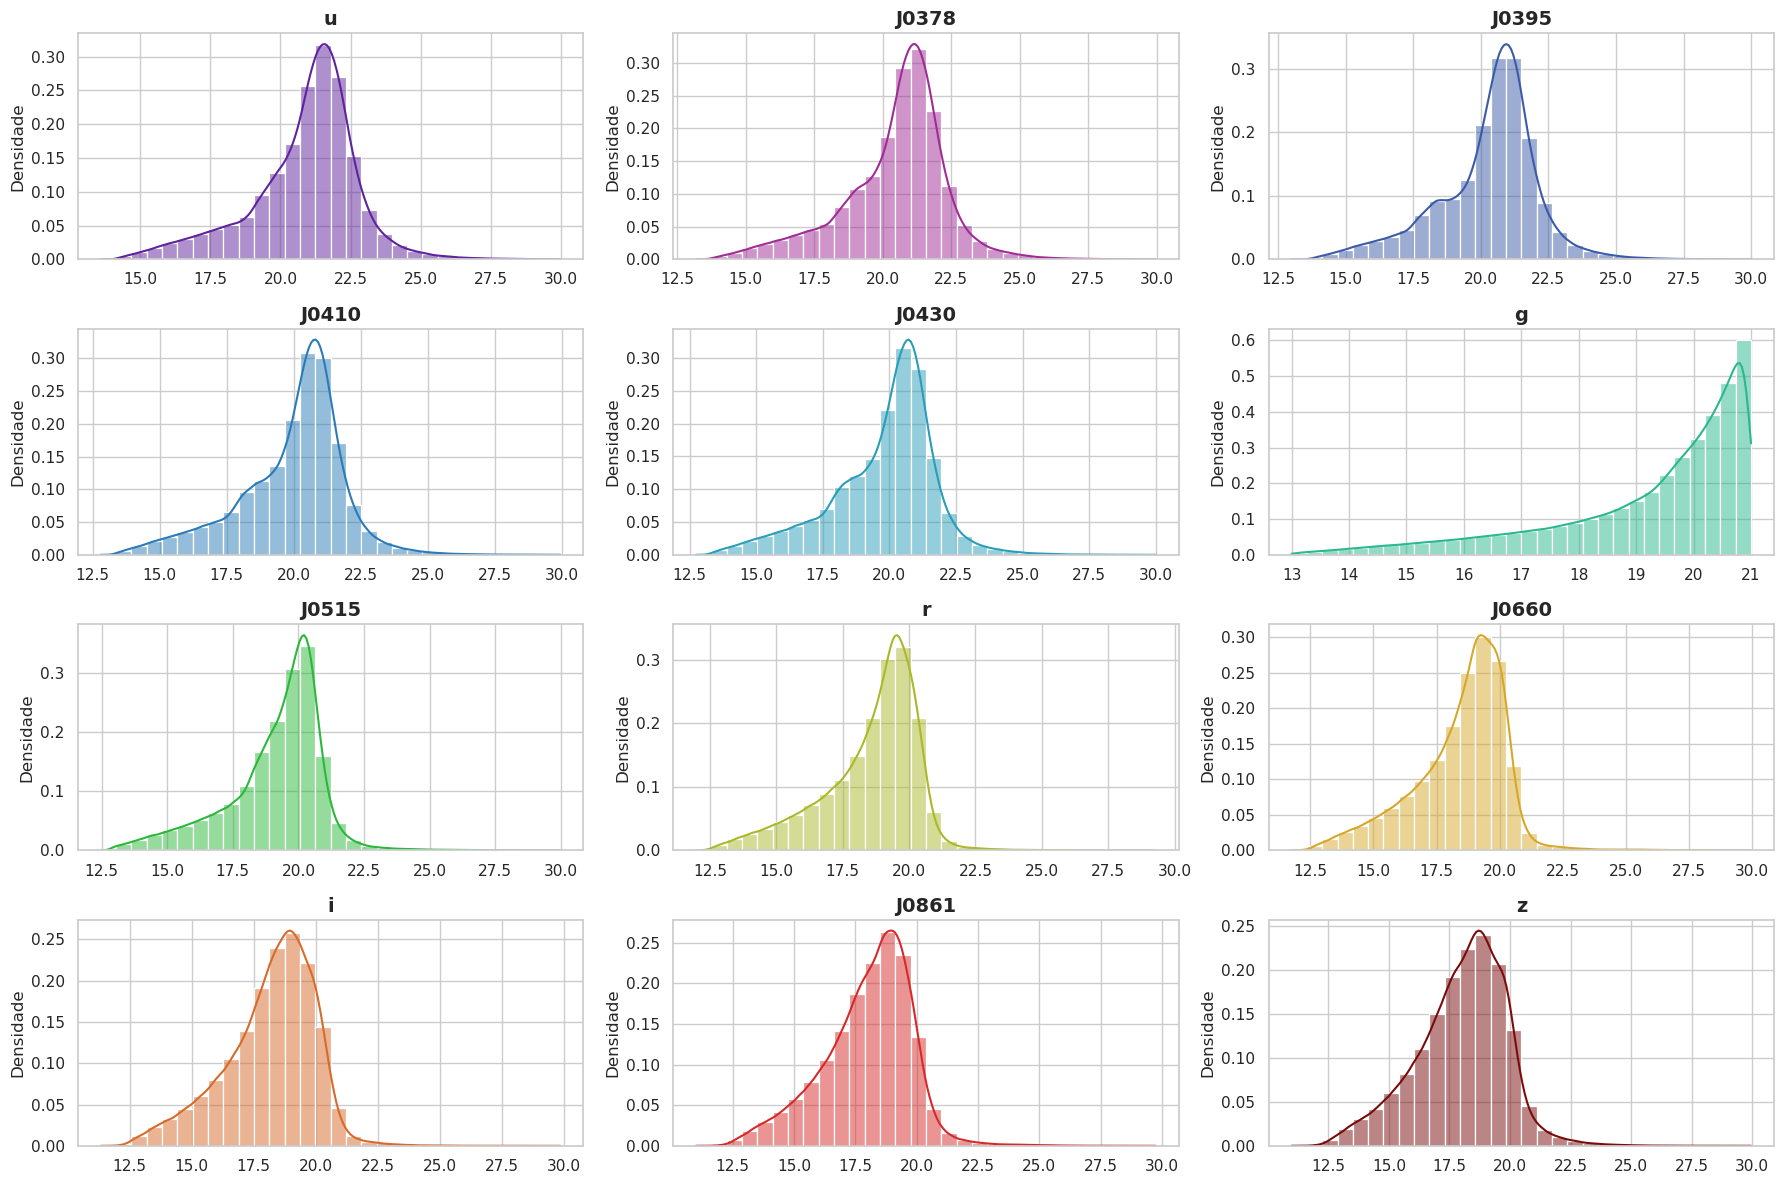
\includegraphics[width=1.0 \columnwidth,angle=0]{hist_distri_mags_data.png}
    \caption[]{Distribuições de densidade das magnitudes corrigidas para extinção nas 12 bandas fotométricas do S-PLUS (APER\_6) após a aplicação dos cortes de qualidade descritos. As bandas incluem 5 de banda larga ($u$, $g$, $r$, $i$, $z$) e 7 de banda estreita (J0378, J0395, J0410, J0430, J0515, J0660, J0861). Os cortes garantem a seleção de objetos com medições fotométricas confiáveis para a análise.}
    \label{fig:hist_distri_mags_data}
    \end{center}
\end{figure}

\chapter{\chapternameanalysis}\label{analise}
Neste capítulo, apresentamos a análise das galáxias ultracompactas (UCDs) no aglomerado de Fornax, com foco nas propriedades das UCDs conhecidas e na seleção de novas candidatas. Inicialmente, discutimos as características das UCDs previamente identificadas e sua distribuição espacial. Em seguida, exploramos a relação entre as UCDs e as galáxias massivas do aglomerado. Também detalhamos o uso de \ac{ML} para classificar objetos compactos e extensos, além de calcular \ac{photoz} para refinar a seleção de candidatas. Por fim, apresentamos a amostra final de candidatas a UCDs e realizamos uma análise comparativa com as UCDs conhecidas e galáxias morfologicamente classificadas.

\section{UCDs em Fornax}\label{sec:ucds_fornax}
Em uma análise inicial, coletamos propriedades das UCDs conhecidas de Fornax na nossa amostra. Utilizamos o catálogo de UCDs conhecidas de \cite{catalog_ucds}, que compila descobertas de outros trabalhos em várias regiões do céu até o ano de sua publicação. Na Figura \ref{distribution_know_ucds}, apresentamos a distribuição espacial das UCDs desse catálogo na região de Fornax. Na Figura \ref{distribuicao_ucds_center} apresentamos a distribuição dessas UCDs apenas na região de Fornax.

\begin{figure}[!ht]
    \centering
    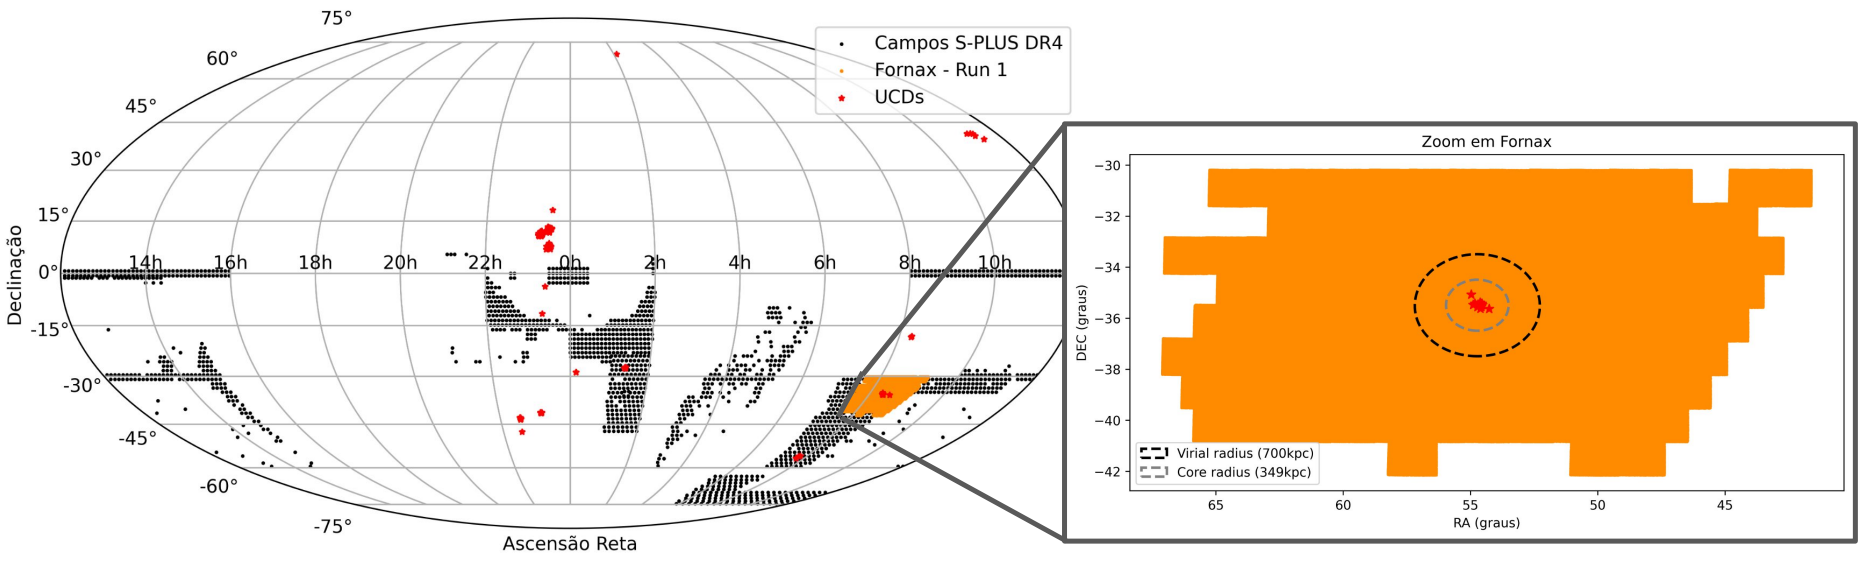
\includegraphics[width=1.\columnwidth,angle=0]{distribution_know_ucds.png}
    \caption[]{Distribuição dos campos observados do S-PLUS DR4 no céu em coordenadas equatoriais. Os pontos pretos representam os campos do S-PLUS DR4, enquanto os pontos vermelhos indicam as UCDs selecionadas como conhecidas vindas de \cite{catalog_ucds}. A área em laranja corresponde ao Aglomerado de Fornax. A imagem mais ao lado é um zoom da região de Fornax.}
    \label{distribution_know_ucds}
\end{figure}

Os objetos compilados presentes na nossa amostra de Fornax tiveram suas propriedades estudadas por \cite{Mieske_2008_2}, onde todos os alvos foram confirmados como pertencentes ao aglomerado por meio de medidas espectroscópicas (\citealt{Drinkwater_2000}, \citealt{Mieske_2002} \& \citeyear{Mieske_2004}, \citealt{Richtler_2004} \& \citeyear{Richtler_2008}). Dessas descobertas, as 5 primeiras UCDs (chamadas de UCDs clássicas) foram encontradas em Fornax por \cite{Drinkwater_2000}.

Dessa lista de UCDs, com 18 na região de Fornax, foi feito um cruzamento com os dados utilizados neste trabalho. Obtivemos 16 objetos correspondentes na nossa amostra. Na Tabela \ref{ucds_fornax_propriedades}, apresentamos a lista dessas UCDs conhecidas e suas propriedades fornecidas por \cite{Mieske_2008_2}.

As duas UCDs que não tiveram correspondência em nossos dados são \textit{FCC47} e \textit{F-17}. De acordo com \cite{Fahrion_2020}, essas UCDs possuem magnitudes absolutas de $M_v = -11.15$ e $M_v = -11.3$, respectivamente. Nas imagens do S-PLUS, essas UCDs são muito fracas e estão localizadas próximas a objetos mais brilhantes, não sendo detectadas com o RUN 1. Considerando suas magnitudes absolutas $M_v$ e o critério de separação entre UCDs e GCs adotado, conforme definido na Seção \ref{subsec:cuts}, iremos excluí-las de nossa amostra de UCDs.

\begin{table}[!ht]
    \centering
    \caption{Propriedades das UCDs identificadas na região de Fornax com dados da amostra deste estudo, fornecidas por \cite{Mieske_2008_2}. As colunas representam: Nome - identificação do objeto; \ac{RA}; \ac{DEC}; Massa Total - massa total do objeto em $10^6 \, M_\odot$; $M/L_V$ - razão massa-luminosidade; [Fe/H] - metalicidade em dex; $r_h$ - raio de meia-luz em parsecs (medido na banda V); $\sigma$ - dispersão de velocidades em km/s.}
    \begin{tabular}{lcccccccc}
        \toprule
        Nome & RA & Dec & Massa Total & $M/L_V$ & [Fe/H] & $r_h$ & $\sigma$ \\
        & (graus) & (graus) & ($10^6 \, M_\odot$) & & (dex) & (pc) & (km/s)\\
        \midrule
        UCD3, F-19 & 54.72542 & -35.55933 & $93.6 \pm 14.0$ & $4.69 \pm 0.70$ & -0.4 & 89.7 & 22.8 \\
        UCD1       & 54.26375 & -35.63461 & $32.1 \pm 3.9$  & $4.99 \pm 0.60$ & -0.7 & 22.4 & 27.1 \\
        F-24       & 54.89958 & -35.47350 & $24.5 \pm 7.8$  & $3.44 \pm 1.10$ & -0.4 & 29.5 & 21.4 \\
        UCD5       & 54.96908 & -35.07336 & $18.0 \pm 4.5$  & $3.37 \pm 0.85$ & -1.2 & 31.2 & 18.7 \\
        F-1a       & 54.52625 & -35.48300 & $16.2 \pm 3.8$  & $2.45 \pm 0.58$ & 0.0  & 23.1 & 18.7 \\
        F-9        & 54.60625 & -35.62853 & $14.1 \pm 3.6$  & $4.72 \pm 1.20$ & -0.8 & 9.1  & 25.7 \\
        F-5        & 54.54500 & -35.42950 & $13.7 \pm 2.4$  & $3.16 \pm 0.55$ & -0.3 & 5.0  & 34.5 \\
        F-6        & 54.56875 & -35.43878 & $12.5 \pm 2.4$  & $5.32 \pm 1.00$ & 0.2  & 7.3  & 27.3 \\
        F-7        & 54.57333 & -35.55067 & $10.5 \pm 1.4$  & $4.21 \pm 0.57$ & -1.3 & 14.9 & 20.1 \\
        F-12       & 54.62083 & -35.38231 & $8.3 \pm 2.9$   & $2.36 \pm 0.83$ & -0.4 & 10.3 & 22.9 \\
        F-11       & 54.61792 & -35.42736 & $5.7 \pm 3.7$   & $1.64 \pm 1.10$ & -0.9 & 3.6  & 26.2 \\
        F-34       & 54.55292 & -35.48250 & $5.5 \pm 1.3$   & $3.17 \pm 0.74$ & -0.9 & 4.0  & 24.6 \\
        F-22       & 54.82375 & -35.42503 & $5.3 \pm 1.0$   & $2.13 \pm 0.39$ & -0.4 & 10.0 & 22.8 \\
        F-53       & 54.66917 & -35.48611 & $3.9 \pm 1.0$   & $2.66 \pm 0.69$ & -0.9 & 4.4  & 19.6 \\
        F-51       & 54.57125 & -35.44203 & $3.5 \pm 0.9$   & $2.38 \pm 0.62$ & -0.8 & 4.2  & 20.1 \\
        F-59       & 54.70375 & -35.46225 & $1.3 \pm 0.6$   & $0.94 \pm 0.43$ & -2.1 & 5.7  & 9.8  \\
        \bottomrule
    \end{tabular}
    \label{ucds_fornax_propriedades}
\end{table}

Fazendo um cruzamento das UCDs conhecidas do catálogo de \cite{catalog_ucds} com os dados da fotometria original do S-PLUS DR4, obtivemos 9 objetos, em comparação com os 16 que obtivemos anteriormente. Isso ressalta a importância da redução da fotometria de Fornax vinda de \cite{haack2024splusfornaxprojectsfp} para a identificação das nossas galáxias de interesse.

Fazendo um cruzamento dessas UCDs com o catálogo GAIA DR3 \citep{GAIA_DR3}, que fornece informações de classificação estrela-galáxia-quasar, observamos que das 16, 8 têm probabilidade maior que 50\% de serem galáxias e 8 têm probabilidade maior que 50\% de serem estrelas. Esse fato mostra a dificuldade da classificação desses objetos. Mostramos na Tabela \ref{tab_ucds_stars_galaxy_like} as médias e desvios padrões das magnitudes dos dados usados desses dois grupos.

\begin{table}[!ht]
    \centering
    \caption{Comparação das 12 magnitudes do S-PLUS DR4 (Run 1) da abertura APER\_6 corrigidas pela extinção entre as UCDs conhecidas, separadas em dois grupos: classificação estrela (PSS > 0,5) ou galáxia (PGal > 0,5) pelo Gaia DR3.}   
    \begin{tabular}{lcccc}
        \toprule
        Filtro & \multicolumn{2}{c}{UCD(PGal>0,5)} & \multicolumn{2}{c}{UCD(PSS>0,5)} \\
        & Média & $\sigma$ & Média & $\sigma$ \\
        \midrule
        u & 21,73 & 0,83 & 22,03 & 0,37 \\
        J0378 & 21,13 & 0,84 & 22,04 & 0,49 \\
        J0395 & 21,29 & 1,04 & 22,42 & 1,23 \\
        J0410 & 20,41 & 0,53 & 21,63 & 0,57 \\
        J0430 & 20,29 & 0,67 & 21,16 & 0,33 \\
        g    & 19,88 & 0,73 & 21,07 & 0,63 \\
        J0515 & 19,60 & 0,63 & 20,75 & 0,46 \\
        r    & 18,08 & 0,67 & 20,41 & 0,36 \\
        J0660 & 19,00 & 0,68 & 20,27 & 0,39 \\
        i    & 18,75 & 0,72 & 20,10 & 0,44 \\
        J861 & 18,58 & 0,69 & 19,82 & 0,36 \\
        z    & 18,54 & 0,72 & 19,98 & 0,51 \\
        \bottomrule
    \end{tabular}
    \label{tab_ucds_stars_galaxy_like}
\end{table}

Concluímos pela Tabela \ref{tab_ucds_stars_galaxy_like} que o grupo de UCDs classificadas como galáxias pelo GAIA DR3 é mais brilhante que o grupo classificado como estrelas. Observando ainda a banda fotométrica $r$, usada como referência devido à sua profundidade e qualidade, temos as UCDs classificadas como galáxias no intervalo de 17,64 a 19,83 magnitudes, enquanto as classificadas como estrelas estão no intervalo de 19,82 a 20,83 magnitudes. Podemos usar estes intervalos como referência para a seleção dos objetos de interesse.

Pelas propriedades da Tabela \ref{ucds_fornax_propriedades}, mostramos na Figura \ref{r_h_M_ucds} a relação entre a massa e o raio de meia-luz das UCDs conhecidas de Fornax. Observamos uma conclusão similar: o grupo de UCDs classificadas como galáxias pelo GAIA DR3 é mais brilhante que o grupo classificado como estrelas, e assim, tem uma relação entre a massa e o raio de meia-luz maior.

\begin{figure}[!ht]
    \centering
    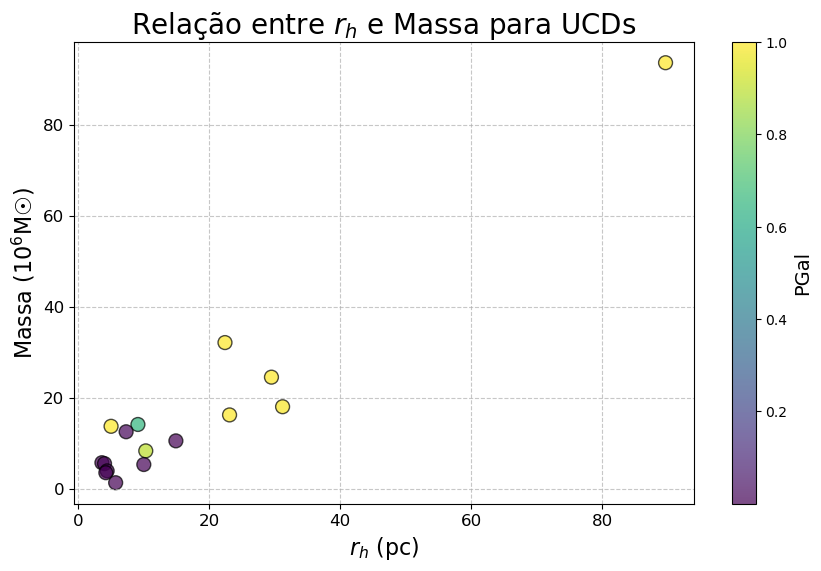
\includegraphics[width=0.8\columnwidth,angle=0]{r_h_M_ucds.png} 
    \caption[]{Relação entre a massa e o raio de meia-luz das UCDs conhecidas de Fornax. Barra de cor pela classificação como galáxia (PGal) vinda do Gaia DR3.}
    \label{r_h_M_ucds}
\end{figure}

Na Figura \ref{distribuicao_fwhm_image_r_r_aper6_ucds_fornax}, mostramos a distribuição de \ac{FWHM} em função da banda \textit{r\_APER\_6} para UCDs de Fornax, coloridas pelo classificador de galáxia (PGal) do Gaia DR3. Percebemos que, para os objetos mais fracos, o classificador do Gaia apresenta maior taxa de erro ao classificá-los, atribuindo maiores probabilidades de serem estrelas. A UCD \textit{F-34} é a que possui o maior valor de \textit{FWHM}. Observando as imagens, não notamos que ela seja significativamente maior que as outras. No entanto, possivelmente devido à sua proximidade com o centro do aglomerado, em uma região contaminada pela envoltória das galáxias mais luminosas, sua fotometria pode ser afetada por outros objetos próximos, aumentando ligeiramente o seu \textit{FWHM} nas detecções.

\begin{figure}[!ht]
    \centering
    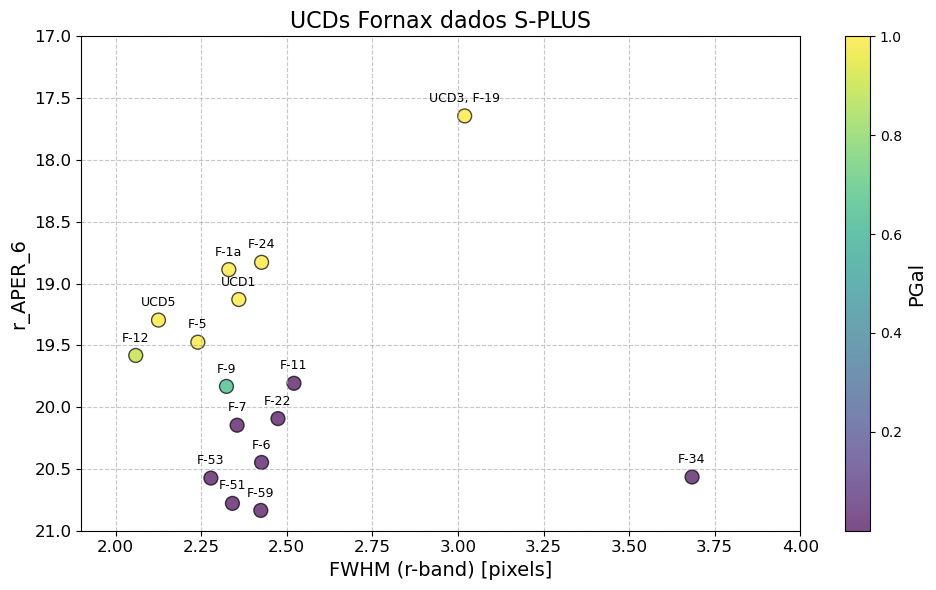
\includegraphics[width=0.8\columnwidth,angle=0]{distribuicao_fwhm_image_r_r_aper6_ucds_fornax.png}
    \caption[]{Distribuição de \textit{FWHM (r-band)} em função da magnitude \textit{r\_APER\_6} para UCDs de Fornax nos dados do S-PLUS.}
    \label{distribuicao_fwhm_image_r_r_aper6_ucds_fornax}
\end{figure}

Usando o compilado de \ac{specz} de \cite{Lima_2024}, mostramos na Tabela \ref{tab:ucds_know_z_gmag} os valores para esses objetos catalogados como UCDs em nossos dados, vindo de \cite{catalog_ucds}, juntamente da magnitude $g$ na abertura $APER\_6$ de referência. Apresentamos também os valores de redshift fotométrico (\textit{zml}) de \citep{erik_photoz_2024}. 

Esses valores foram obtidos a partir da fotometria padrão do S-PLUS. Assim, parte das UCDs não possui valores de redshift fotométrico, pois algumas estão presentes apenas com a redução da fotometria do RUN 1. Os valores de \textit{zml} são superiores aos valores de \textit{specz}, refletindo o problema de que, para a amostra de objetos com redshifts fotométricos, temos muito menos dados em redshifts próximos. Assim, os classificadores tendem a superestimar os valores. Ainda assim, eles são úteis para avaliar os objetos de fundo. Detalhamos mais sobre a utilização deles na seção \ref{sec:zphot}.

\begin{table}[!ht]
    \centering
    \caption{Valores de \ac{specz} provenientes de \cite{Lima_2024} e magnitudes $g$ e abertura $APER\_6$ obtidas dos dados fotométricos utilizados neste trabalho. Redshifts fotométricos (\textit{zml}) de \cite{erik_photoz_2024}.}
    \begin{tabular}{lccc}
        \toprule
        Nome & spec-$z$ & $g$ & zml \\
        \midrule
        UCD3 & 0.0053 & 18.47 & 0.03\\
        UCD1 & 0.0052 & 19.75 & 0.08\\
        F-24 & 0.0063 & 19.66 & 0.04\\
        UCD5 & 0.0045 & 19.71 & 0.04\\
        F-1a & 0.0042 & 19.66 & -\\
        F-9  & 0.0058 & 20.85 & 0.07\\
        F-5  & 0.0057 & 20.54 & -\\
        F-6  & 0.0037 & 20.48 & -\\
        F-7  & 0.0050 & 20.89 & 0.16\\
        F-12 & 0.0055 & 20.37 & -\\
        F-11 & 0.0059 & 20.40 & -\\
        F-34 & 0.0054 & 20.79 & -\\
        F-22 & 0.0034 & 20.69 & 0.06\\
        F-53 & 0.0020 & 21.57 & -\\
        F-51 & 0.0041 & 22.23 & -\\
        F-59 & 0.0061 & 21.47 & -\\
        \bottomrule
    \end{tabular}
    \label{tab:ucds_know_z_gmag}
\end{table}

Conforme definido na seção \ref{subsec:cuts}, consideraremos como UCDs os objetos com magnitudes $g$ menores que 21. Assim, da Tabela \ref{tab:ucds_know_z_gmag}, iremos remover os objetos mais fracos que 21.

\subsection{Distribuição relativa ao centro de Fornax}
Na Figura \ref{distribuicao_ucds_center}, apresentamos a distribuição de UCDs, com respeito ao centro do aglomerado, onde temos a galáxia NGC 1399, que é a galáxia mais massiva do aglomerado de Fornax.

\begin{figure}[!ht]
    \begin{center}
    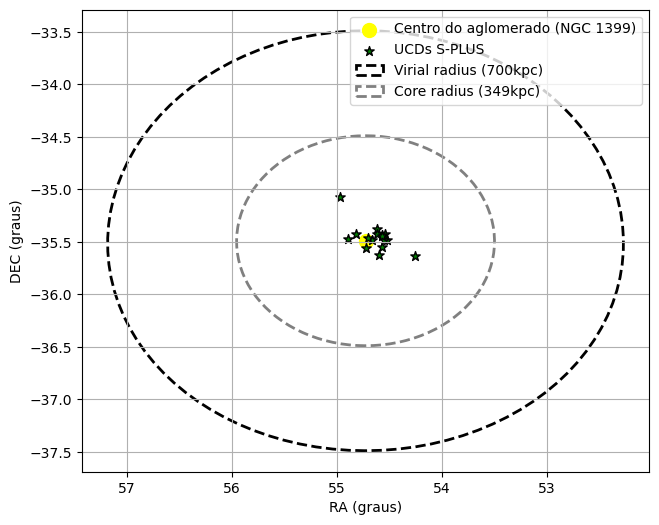
\includegraphics[width=0.9\columnwidth,angle=0]{distribuicao_ucds_center.png}
    \caption[]{Distribuição das UCDs conhecidas de Fornax nos dados do S-PLUS. Os pontos azuis representam as UCDs conhecidas, coloridas pelo raio de virial (virial radius) e o raio do núcleo (core radius). Centro do aglomerado representado pelo círculo amarelo (NGC 1399), em \ac{RA} = 54.73 e \ac{DEC} = -35.49.}
    \label{distribuicao_ucds_center}
    \end{center}
\end{figure}

Nesta figura, apresentamos a distribuição das UCDs nos dados do S-PLUS, destacando o raio de virial ($virial \, radius$) e o raio do núcleo ($core \, radius$). Utilizamos o $virial \, radius$ como 700 kpc \citep{Drinkwater_2001} e definimos o $core \, radius$ como aproximadamente 349 kpc, assim como feito por \cite{Saifollahi_2021}, o que corresponde a 1 grau no céu (aproximadamente metade do raio de virial). Essa representação evidencia que os objetos estão concentrados no centro do aglomerado.

Para a conversão de kpc para graus, usamos a relação:

\begin{equation}
    \theta = \frac{d}{D} \times \frac{180}{\pi}
\end{equation}
onde $d$ é distância projetada em kpc, $D$ é a distância em kpc até o objeto, e $\theta$ é distância projetada em graus. Considerando que Fornax está a aproximadamente $20 \, \text{Mpc}$ \citep{Blakeslee_2009}, o que corresponde a um módulo de distância de $31.51 \, \text{mag}$, nessa distância, 1 grau equivale a $0.349 \, \text{Mpc}$. Assim, para as propriedades de Fornax, adotamos os valores apresentados na Tabela \ref{tab:properties_fornax}.

% \begin{table}[!ht]
%     \centering    
%     \caption{Propriedades do aglomerado de Fornax. As referências são indicadas por números sobrescritos nos parâmetros: ¹\citealp{Drinkwater_2001}, ²\citealp{Blakeslee_2009}, ³\citealp{Maddox_2019}, ⁴\citealp{Saifollahi_2021}.}   
%     \begin{tabular}{lc}
%         \toprule
%         Parâmetro &  Valor\\
%         \midrule
%         Massa ($M_\odot$)¹ & $7\pm 2. 10^{13}$ \\
%         Raio Virial ($Mpc$)¹ & 0.7 \\
%         Raio Virial ($graus$)¹ & 2 \\
%         Raio interno ($Mpc$)⁴ & 0.349 \\
%         Raio interno ($graus$)⁴ & 1 \\
%         Dispersão de velocidade ($km s^{-1}$)³ & 318 \\
%         Modulo de distância ($mag$)² & 31.51 \\
%         \bottomrule
%     \end{tabular}
%     \label{tab:properties_fornax}
% \end{table}


\begin{table}[!ht]
    \centering    
    \caption{Propriedades do aglomerado de Fornax. As referências são indicadas por números sobrescritos nos parâmetros: $^1$\citealp{Drinkwater_2001}, $^2$\citealp{Blakeslee_2009}, $^3$\citealp{Maddox_2019}. Definição do \textit{Raio interno (core radius)} vinda de $^4$\cite{Saifollahi_2021}.}   
    \begin{tabular}{lc}
        \toprule
        Parâmetro &  Valor\\
        \midrule
        Massa ($M_\odot$)$^1$ & $7\pm 2. 10^{13}$ \\
        Raio Virial ($Mpc$)$^1$ & 0.7 \\
        Raio Virial ($graus$)$^1$ & 2 \\
        Raio interno ($Mpc$)$^4$ & 0.349 \\
        Raio interno ($graus$)$^4$ & 1 \\
        Dispersão de velocidade ($km s^{-1}$)$^3$ & 318 \\
        Modulo de distância ($mag$)$^2$ & 31.51 \\
        \bottomrule
    \end{tabular}
    \label{tab:properties_fornax}
\end{table}

Na Figura \ref{distribuicao_ucds_center}, observamos que as UCDs conhecidas estão concentradas no centro do aglomerado. A presença de UCDs no centro é consistente com outros estudos, que também identificaram essas estruturas em regiões de alta densidade de galáxias massivas. No entanto, esse padrão pode estar relacionado ao viés das pesquisas espectroscópicas, que tendem a se concentrar nas áreas centrais do aglomerado, e não necessariamente reflete a distribuição real das UCDs em Fornax.

% Para ilustrar melhor a distribuição espacial das UCDs em Fornax, também é útil apresentar as regiões com a presença das principais galáxias massivas encontradas. A presença e a distribuição das galáxias massivas são importantes, pois, além do centro do aglomerado, onde as UCDs estão mais concentradas, as galáxias massivas também podem desempenhar um papel relevante na localização dessas estruturas. Segundo o cenário de {\it tidal stripping}, as UCDs podem ser formadas a partir da interação com uma galáxia mais massiva. Assim, quando uma galáxia anã nucleada começa a interagir com uma galáxia mais massiva, após algumas passagens orbitais, parte de sua matéria pode ser removida, resultando no núcleo remanescente, que observamos como sendo uma UCD.

As UCDs em Fornax estão concentradas no centro do aglomerado e próximas a galáxias massivas. Segundo o cenário de {\it tidal stripping}, essas estruturas podem se formar quando galáxias anãs nucleadas interagem com galáxias massivas, perdendo matéria após passagens orbitais e deixando apenas o núcleo remanescente, observado como uma UCD.

Selecionamos as galáxias mais luminosas confirmadas do aglomerado (\citealp{Ferguson_1989}, \citealp{Jordan_2007}, \citealp{Venhola_2018}) utilizando o catálogo de \cite{Lima_2024}, dentro da faixa de redshift do aglomerado de Fornax ($0,003\leq z\leq0,006$). Para identificar as galáxias mais massivas entre esses objetos, realizamos um corte na magnitude absoluta $M_r$, utilizando a abertura de 6 arcsecs. Calculamos a magnitude absoluta com base no módulo de distância da Tabela \ref{tab:properties_fornax} e na magnitude aparente $m_r$ dos objetos. Assim como em \cite{Saifollahi_2021}, adotamos um corte em $M_r \leq -18$ para a seleção das galáxias massivas.

Na Figura \ref{distribuicao_galaxias_massivas} na imagem superior, apresentamos a distribuição espacial das galáxias massivas em Fornax. Acrescentamos em cada uma delas um raio de 200 kpc. Esse valor é comparável com o raio de virial da Via Lactea ($R_{vir}\sim 200kpc$, \cite{Dehnen_2006}). Apresentamos ainda na Figura \ref{distribuicao_galaxias_massivas}, na imagem inferior, a mesma distribuição sobreposta a uma imagem do aglomerado de Fornax, criada com as imagens do Legacy Survey. Verificamos que as UCDs conhecidas estão mais associadas ao centro do aglomerado que às galáxias massivas.

\begin{figure}[!ht]
\centering
\captionsetup{justification=centering}
\begin{subfigure}[b]{0.75\textwidth}
    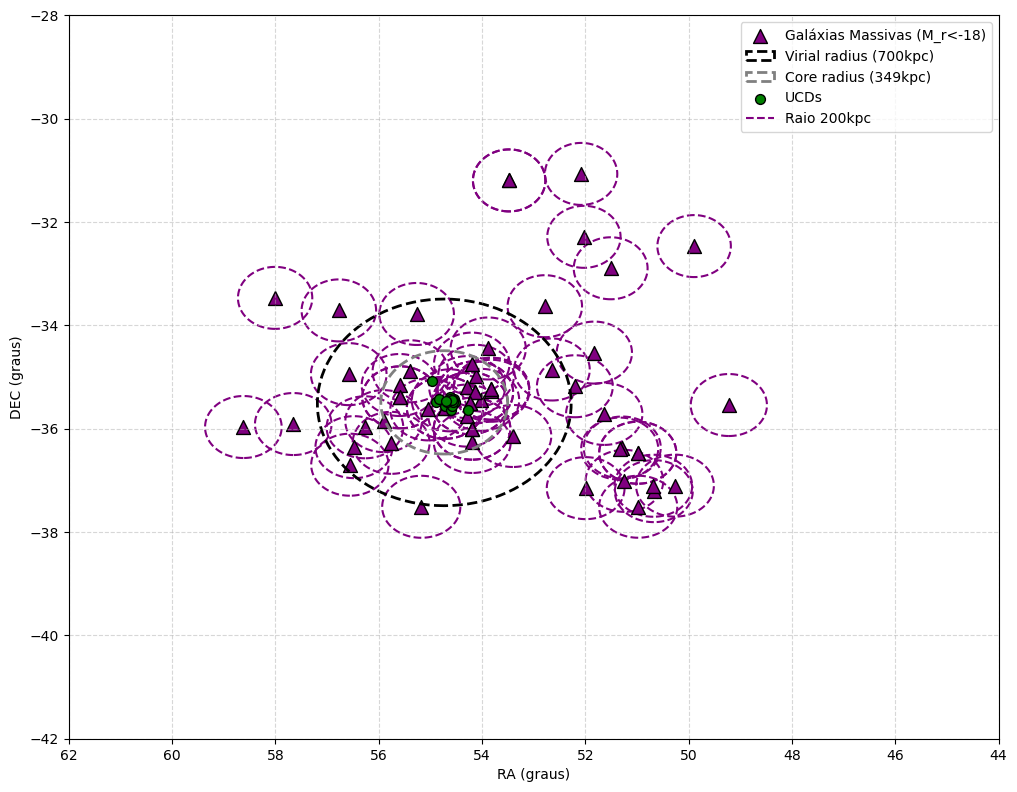
\includegraphics[width=\textwidth]{distribuicao_galaxias_massivas.png}
    \caption{}
\end{subfigure}
\begin{subfigure}[b]{0.75\textwidth}
    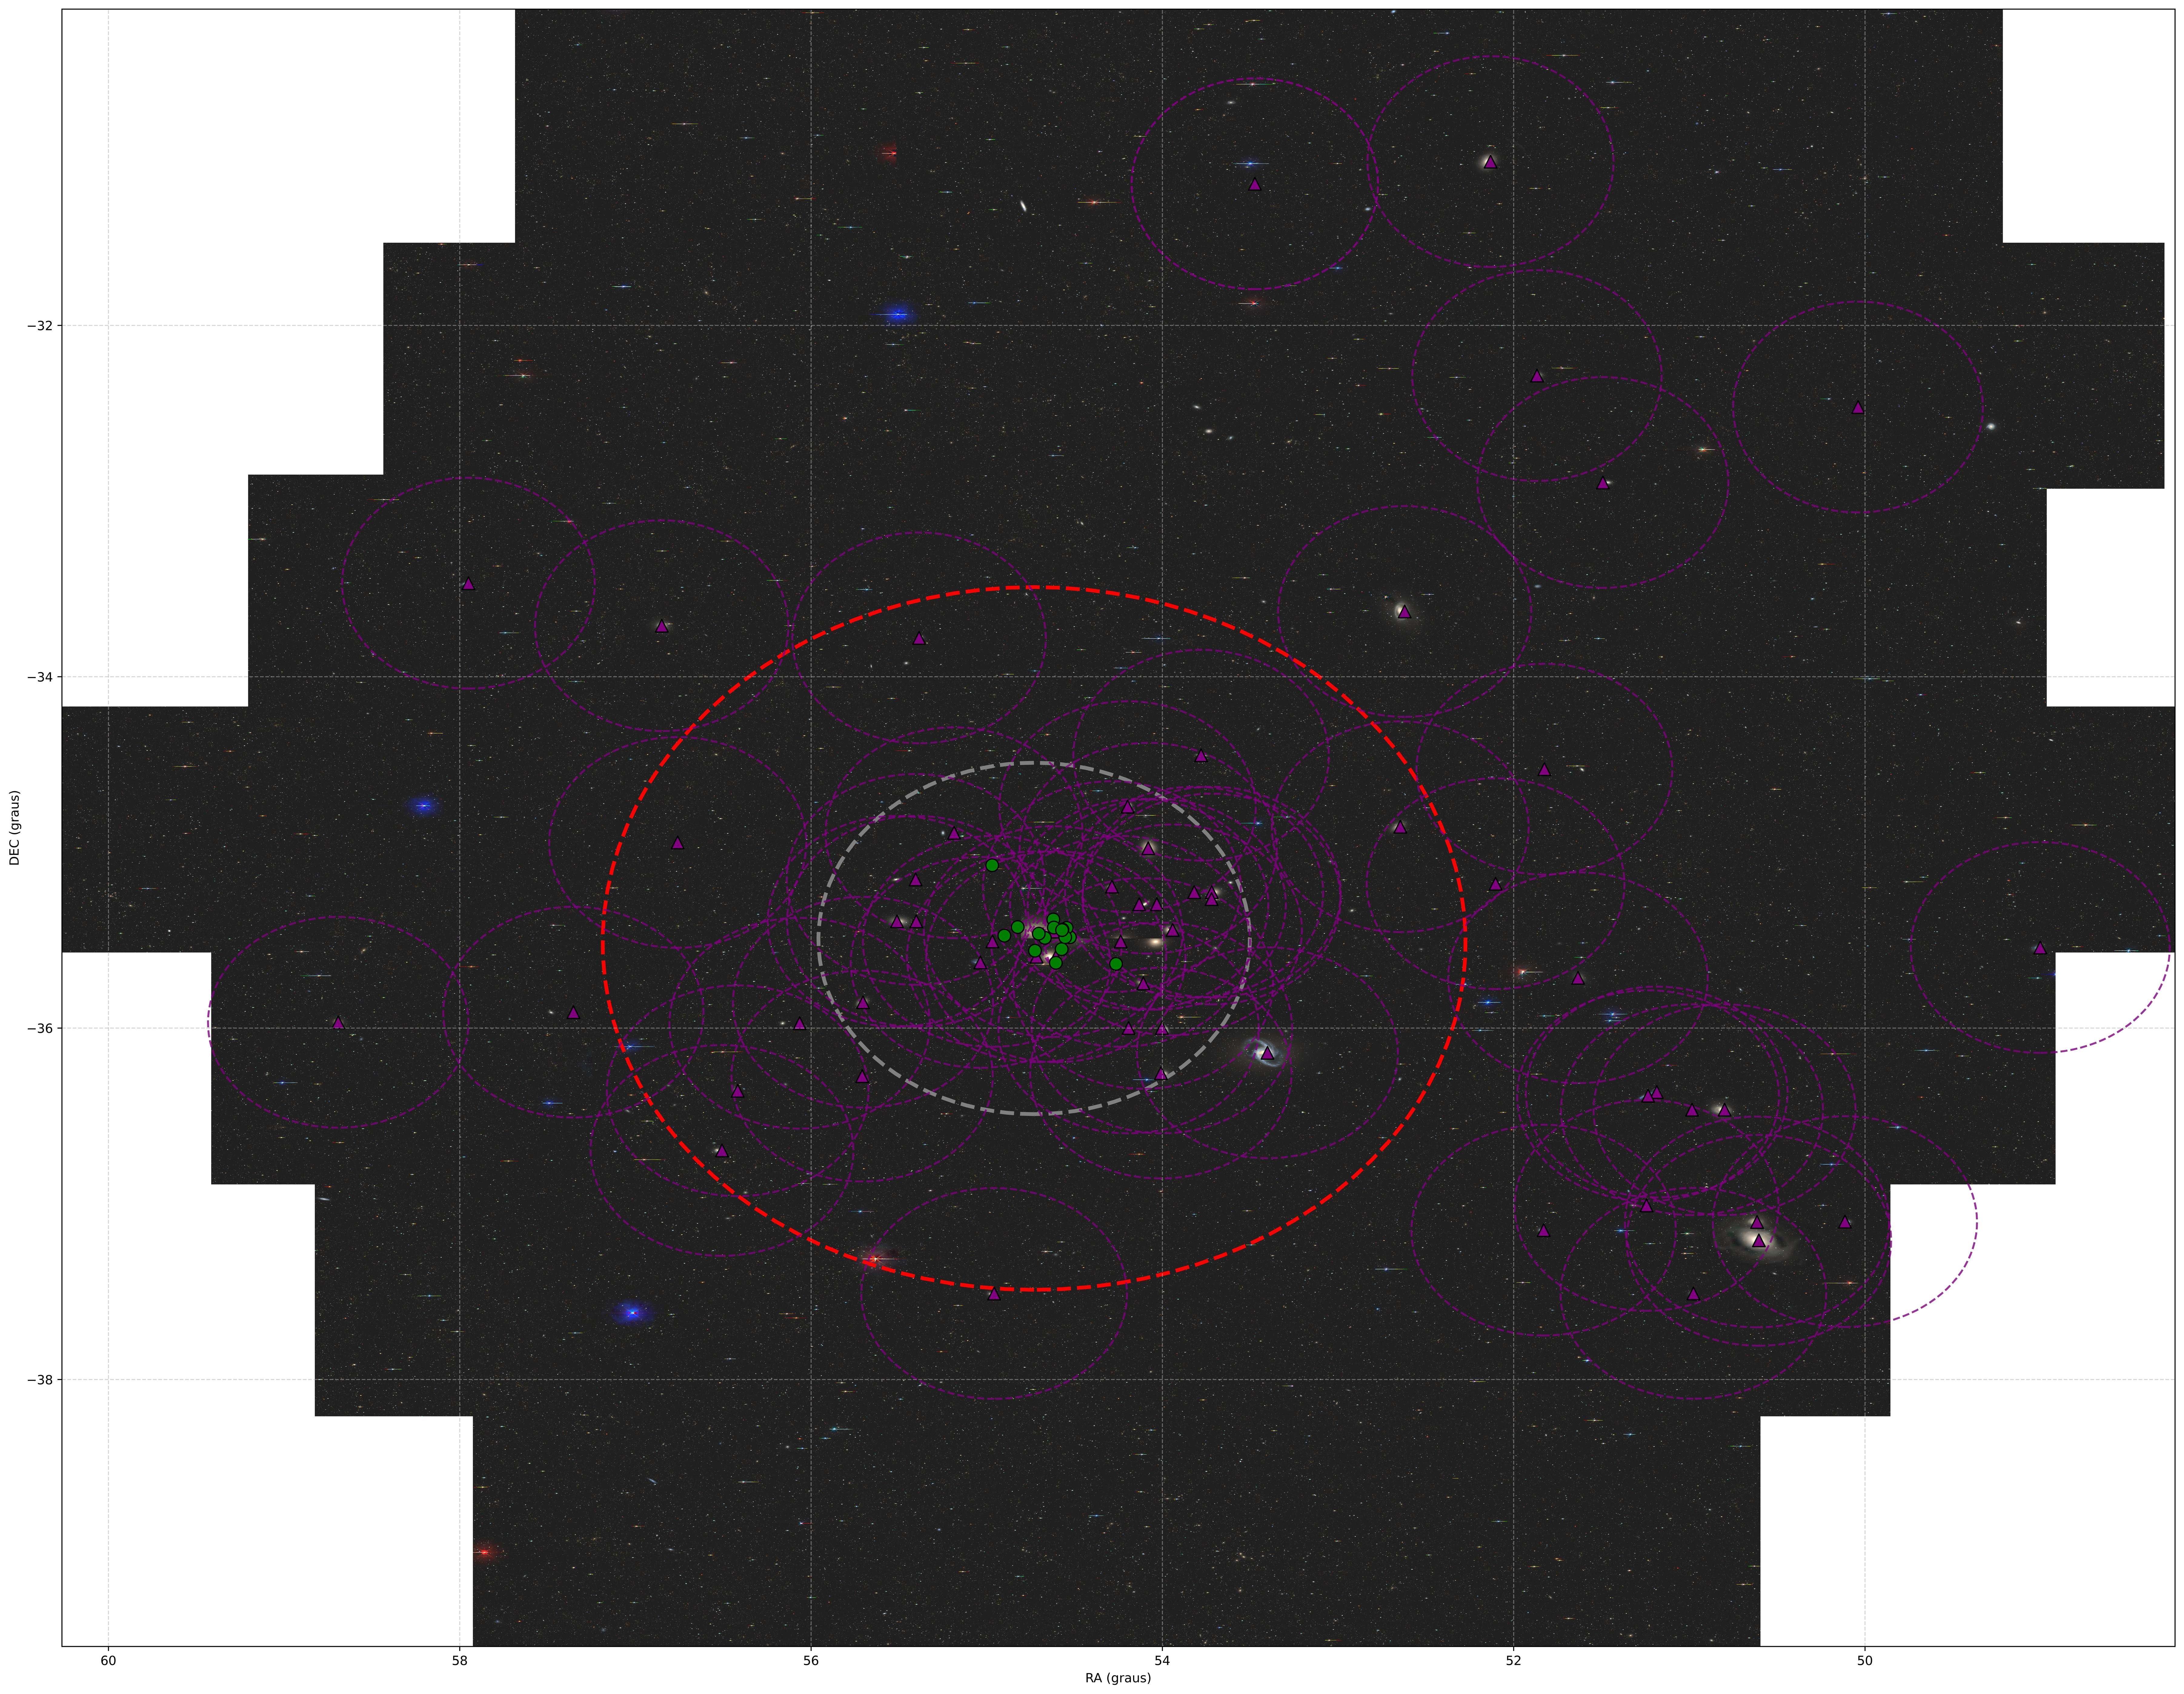
\includegraphics[width=\textwidth]{fields_fornax_center_migue_compress.jpg}
    \caption{}
\end{subfigure}
\caption{(a) Distribuição das galáxias massivas em Fornax nos dados do S-PLUS. Pontos em verde são as UCDs. Os pontos em roxo representam as galáxias massivas, com um círculo indicando um raio de 200 kpc ao redor de cada uma. O arco preto corresponde ao raio de virial de Fornax, estimado em 700 kpc, enquanto o arco cinza representa o raio do núcleo (core radius), definido como 349 kpc.\\ (b) Mesma imagem com a adição ao fundo da imagem real do aglomerado de Fornax, criada com as imagens do Legacy Survey. O círculo vermelho é o raio do Virial e o branco o do núcleo.}
\label{distribuicao_galaxias_massivas}
\end{figure}

% Observamos dois picos de magnitudes, um em torno de -13 e outro em torno de -19. Os dois picos na distribuição de $M_r$ têm origens distintas e estão relacionados tanto à função de luminosidade intrínseca do aglomerado de Fornax quanto aos limites de detecção do levantamento. O pico em torno de -19 coincide aproximadamente com o joelho da função de Schechter das galáxias em aglomerados: é onde a densidade de galáxias gigantes (elípticas e lenticulares do núcleo de Fornax, como NGC 1399) é mais alta antes de cair exponencialmente. O pico em torno de -13 está correlacionado ao limite de completude do catálogo para os objetos mais fracos ou mais distantes. Assim que chegamos perto do limite de detecção, o número de objetos cai abruptamente para além desse valor.

\section{Procura de UCDs com Aprendizado de Máquina}\label{sec:aprendizado_maquina}
Neste trabalho, utilizamos aprendizado de máquina (\ac{ML}) para auxiliar na identificação de candidatas a galáxias ultracompactas (UCDs) no aglomerado de Fornax, com base em dados fotométricos do S-PLUS. A distinção entre UCDs e outros objetos compactos, como estrelas ou aglomerados globulares, é desafiadora. Para abordar essa dificuldade, empregamos um método supervisionado que classifica os objetos em duas categorias principais com base exclusivamente na fotometria: compactos e extensos. Essa abordagem permite identificar objetos compactos com características fotométricas semelhantes às de galáxias, facilitando a seleção de candidatas a UCDs.

O processo é dividido em duas etapas principais. Primeiro, classificamos os objetos em duas categorias: compactos e extensos, com base exclusivamente na \ac{FWHM}. Objetos compactos, como estrelas e UCDs, possuem valores menores de \textit{FWHM}, enquanto objetos extensos, como galáxias, apresentam valores maiores. Essa classificação inicial é feita para separar os objetos com base em sua morfologia.

Na segunda etapa, utilizamos um classificador supervisionado treinado exclusivamente com os dados fotométricos dos objetos. Como a imensa maioria dos objetos extensos são galáxias e a maioria dos objetos compactos são estrelas, o objetivo do classificador é identificar, dentro do grupo de objetos compactos, aqueles que possuem características fotométricas semelhantes às de galáxias extensas. Esses objetos compactos, classificados como extensos pelo modelo, são então considerados candidatos a UCDs.

Em resumo, a proposta consiste em explorar a morfologia dos objetos para separá-los em compactos e extensos e, em seguida, utilizar a fotometria para identificar candidatos a UCDs entre os objetos compactos. Nas subseções seguintes, detalharemos o processo de construção da amostra de treino, o tratamento de valores faltantes, o treinamento do modelo e a avaliação do desempenho do classificador.



\subsection{Amostra de treino}\label{subsec:amostra_treino}
Para a amostra de treino, é desejável implementar uma estratégia que auxilie na identificação de candidatas a UCDs. Uma abordagem comum é a utilização de um classificador, onde um modelo é treinado com um conjunto de dados rotulados e, posteriormente, é capaz de classificar novos objetos com base nas características aprendidas durante o treinamento.

Um exemplo semelhante é o problema de classificação de quasares, que são fontes pontuais facilmente confundidas com estrelas, mas possuem características fotométricas que os distinguem destas. Nesse caso, um modelo de classificação pode ser treinado com dados de quasares e estrelas, realizando a separação entre eles. No entanto, para UCDs, temos uma quantidade limitada de objetos conhecidos, impossibilitando um conjunto de dados grande o suficiente para treinar um modelo de classificação direta de UCDs.

Para a identificação de objetos compactos e extensos, usamos a \textit{FWHM} normalizada para cada uma das bandas. O valor normalizado é dado pela \textit{FWHM} do objeto dividido pela \textit{FWHM} média do campo. A normalização é feita para garantir que a largura do perfil de intensidade seja independente da qualidade da imagem e da região observada, quando comparada entre objetos de diferentes campos.

As estrelas, por sua natureza, são fontes pontuais; por isso, esperamos que a \textit{FWHM} desses objetos seja menor do que a de objetos extensos, como as galáxias, exceto, claro, para galáxias ultra compactas.

Realizamos um cruzamento de dados de treinamento com o catálogo GAIA DR3 \citep{GAIA_DR3}, que fornece informações de classificação estrela-galáxia-quasar. Com esses dados, selecionamos um subconjunto de objetos com as probabilidades de serem estrelas e galáxias maiores que 90\%. A partir desse subconjunto, analisamos a distribuição dos valores de \textit{FWHM} para estrelas e galáxias em cada banda fotométrica.

Na Figura \ref{distribution_of_stars_and_galaxies}, apresentamos um histograma da distribuição de \textit{FWHM} para estrelas e galáxias na banda $r$. Optamos por utilizar a banda $r$ como referência devido à sua maior profundidade, além de observarmos que, em comparação com outras bandas, os picos de \textit{FWHM} para estrelas e galáxias estão mais bem separados, facilitando a distinção entre as duas classes. A Figura \ref{distribution_of_stars_and_galaxies_u} monstra um dos outros exemplos de bandas, a banda $u$. Vemos que a separação entre as duas classes não é tão clara quanto na banda $r$, e o mesmo ocorre para as outras bandas. Portanto, a banda $r$ é a mais adequada para o nosso estudo. 


\begin{center}
    \begin{minipage}{0.45\textwidth}
        \centering
        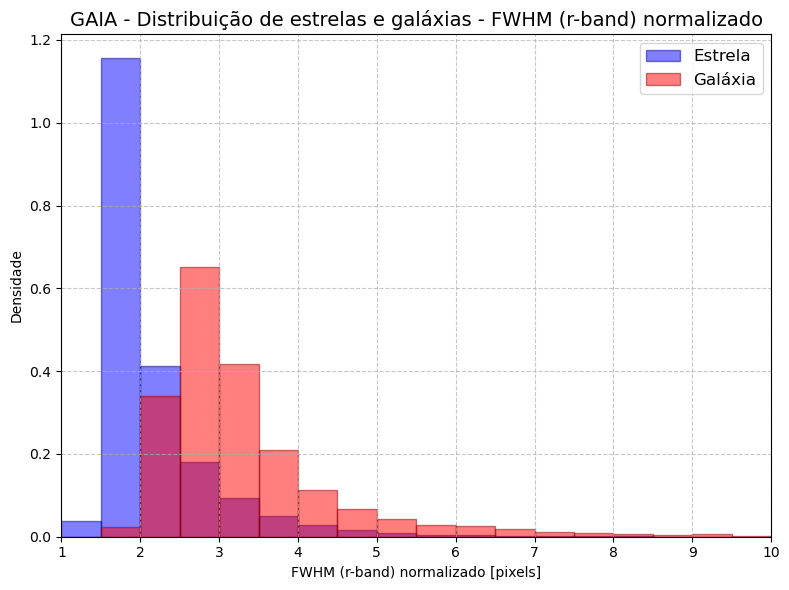
\includegraphics[width=\linewidth]{distribution_of_stars_and_galaxies.png}
        \captionsetup{}
        \captionof{figure}{Histograma da distribuição de \textit{FWHM (r-band) normalizada} dos objetos do cruzamento do S-PLUS DR4 de Fornax, com o catálogo GAIA DR3 com a classificação para estrelas e galáxias com probabilidade maior que 90\%.}  
        \label{distribution_of_stars_and_galaxies}
    \end{minipage}
    \hfill
    \begin{minipage}{0.45\textwidth}
        \centering
        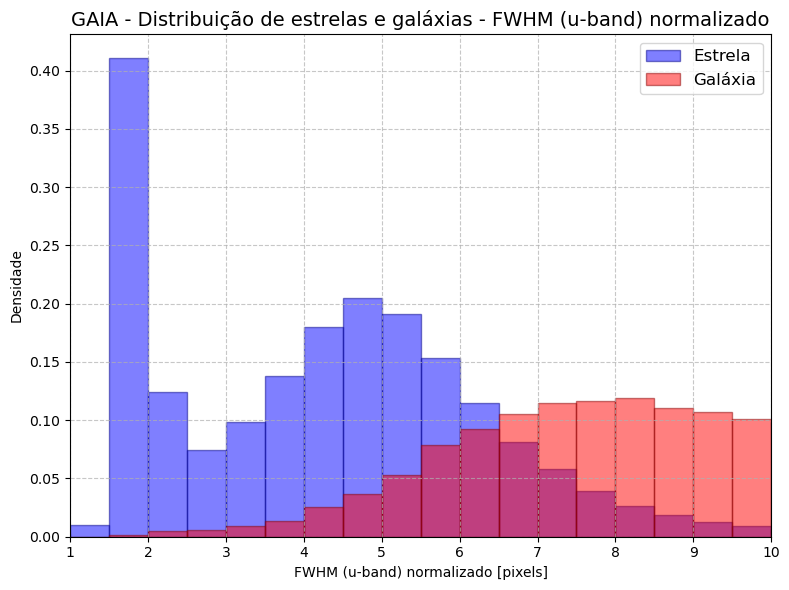
\includegraphics[width=\linewidth]{distribution_of_stars_and_galaxies_u.png}
        \captionsetup{}
        \captionof{figure}{Histograma da distribuição de \textit{FWHM (u-band) normalizada} dos objetos do cruzamento do S-PLUS DR4 de Fornax, com o catálogo GAIA DR3 com a classificação para estrelas e galáxias com probabilidade maior que 90\%.}
        \label{distribution_of_stars_and_galaxies_u}
    \end{minipage}
\end{center}

Há uma diferença entre os picos das distribuições de \textit{FWHM} para estrelas e galáxias. Portanto, o objetivo é definir um corte na \textit{FWHM} para selecionar dois conjuntos: um contendo objetos compactos e outro contendo objetos extensos. No conjunto de objetos compactos, predominam as estrelas, enquanto no conjunto de objetos extensos, as galáxias são mais representativas.

A hipótese é que o modelo aprenda a distinguir as propriedades fotométricas de estrelas e galáxias independentemente da morfologia (ou FWHM) do objeto; numa segunda etapa, procuramos entre os objetos com morfologia estelar aqueles cuja fotometria indica que têm alta probabilidade de serem galáxias.

É importante destacar que, além das galáxias compactas, existem estrelas que possuem espectros muito semelhantes aos das galáxias, especialmente com baixa resolução espectral ou em levantamentos fotométricos. Essas estrelas podem ser confundidas com galáxias, levando também a uma contaminação na amostra de galáxias.

Para identificar, na Figura \ref{distribution_of_stars_and_galaxies}, a melhor divisão entre as duas classes, estabelecemos alguns cortes em \textit{FWHMn} visando encontrar aquele que melhor separa cada população, minimizando a contaminação entre as duas populações. Para cada corte, definimos duas variáveis: Pureza e Completeza, ambas com respeito às galáxias (estas quantidades estão definidas mais formalmente na seção \ref{subsec:analise_modelo}). A Pureza é uma métrica que representa a proporção de galáxias corretamente identificadas em relação ao total de objetos que foram classificados como galáxias. Ela também é conhecida como precisão, sendo sua definição dada na equação \ref{eq:precisao}.

Por outro lado, a Completeza representa a fração de galáxias corretamente identificadas em relação ao número total de galáxias presentes na amostra original, fornecendo uma estimativa de quantas galáxias foram perdidas durante o processo de seleção. Ela é definida na equação \ref{eq:completeza}.

A Figura \ref{purity_completeness} ilustra as métricas de Pureza e Completeza em função da FWHMn. Cada valor de \textit{FWHMn} no gráfico representa o ponto onde separamos as duas classes, sendo as métricas calculadas com referência ao grupo das galáxias. Apresentamos também as curvas do produto entre Pureza e Completeza, juntamente com o F1-score. O ponto ideal para a separação das classes é identificado no valor máximo do F1-score. Esse ponto representa o corte que faremos para a separação entre as duas.

\begin{figure}[!ht]
    \centering
    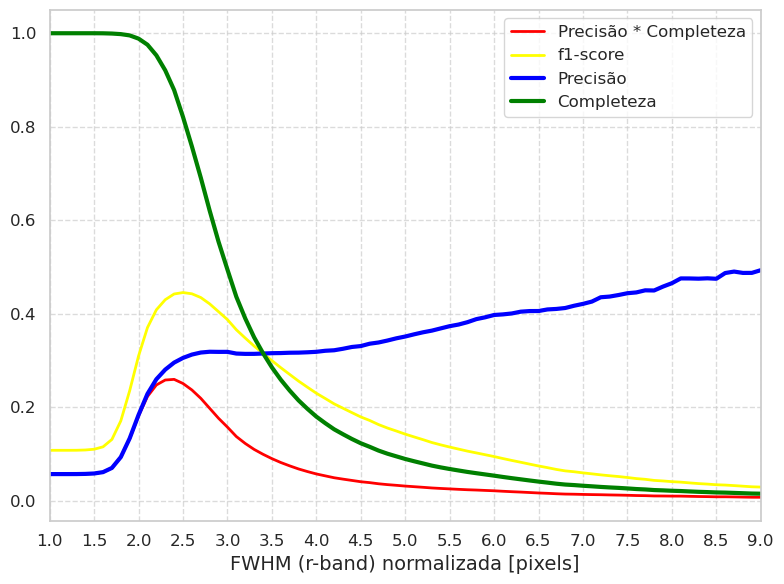
\includegraphics[width=0.95\columnwidth,angle=0]{purity_completeness.png}
    \caption[]{Relação entre Pureza, Completeza e F1-score para diferentes cortes de \textit{FWHM}. O ponto ideal para a separação das classes é identificado no valor máximo do F1-score. Esse ponto representa o corte que faremos para separação entre as duas classes.}
    \label{purity_completeness}
\end{figure}

O valor máximo selecionado para o corte corresponde a um \textit{FWHM (r-band)} de 2,5 pixels. Esse corte representa o ponto de maximização para a separação das classes de acordo com o critério F1-score, com as galáxias associadas à classe de objetos extensos. No entanto, após alguns testes, decidimos realizar um corte para objetos compactos com \textit{FWHM} menores que 2 pixels, o que apresentou melhores resultados nos classificadores iniciais testados. Assim, para a amostra de treino, os objetos com \textit{FWHM (r-band)} menores que 2 pixels são considerados compactos, enquanto os objetos com \textit{FWHM (r-band)} maiores que 2,5 pixels são considerados extensos. Os demais cortes para a seleção de objetos compactos e extensos são descritos na subseção \ref{subsec:cuts}.

Os objetos com valores de \textit{FWHM} entre 2 e 2,5 pixels são considerados indefinidos, ou seja, não são classificados como compactos nem extensos para a amostra de treino devido à incerteza na classificação. No entanto, esses dados ainda serão utilizados na busca por candidatas a UCDs, aplicando o modelo treinado. Assim, esses objetos não são incluídos no treinamento do modelo, mas permanecem na amostra de análise.

Na Figura \ref{amostra_treino}, temos a magnitude \textit{g\_APER\_6} em função da \textit{FWHM (r-band)} para a divisão entre as duas classes adotadas.

\begin{figure}[!ht]
    \centering
    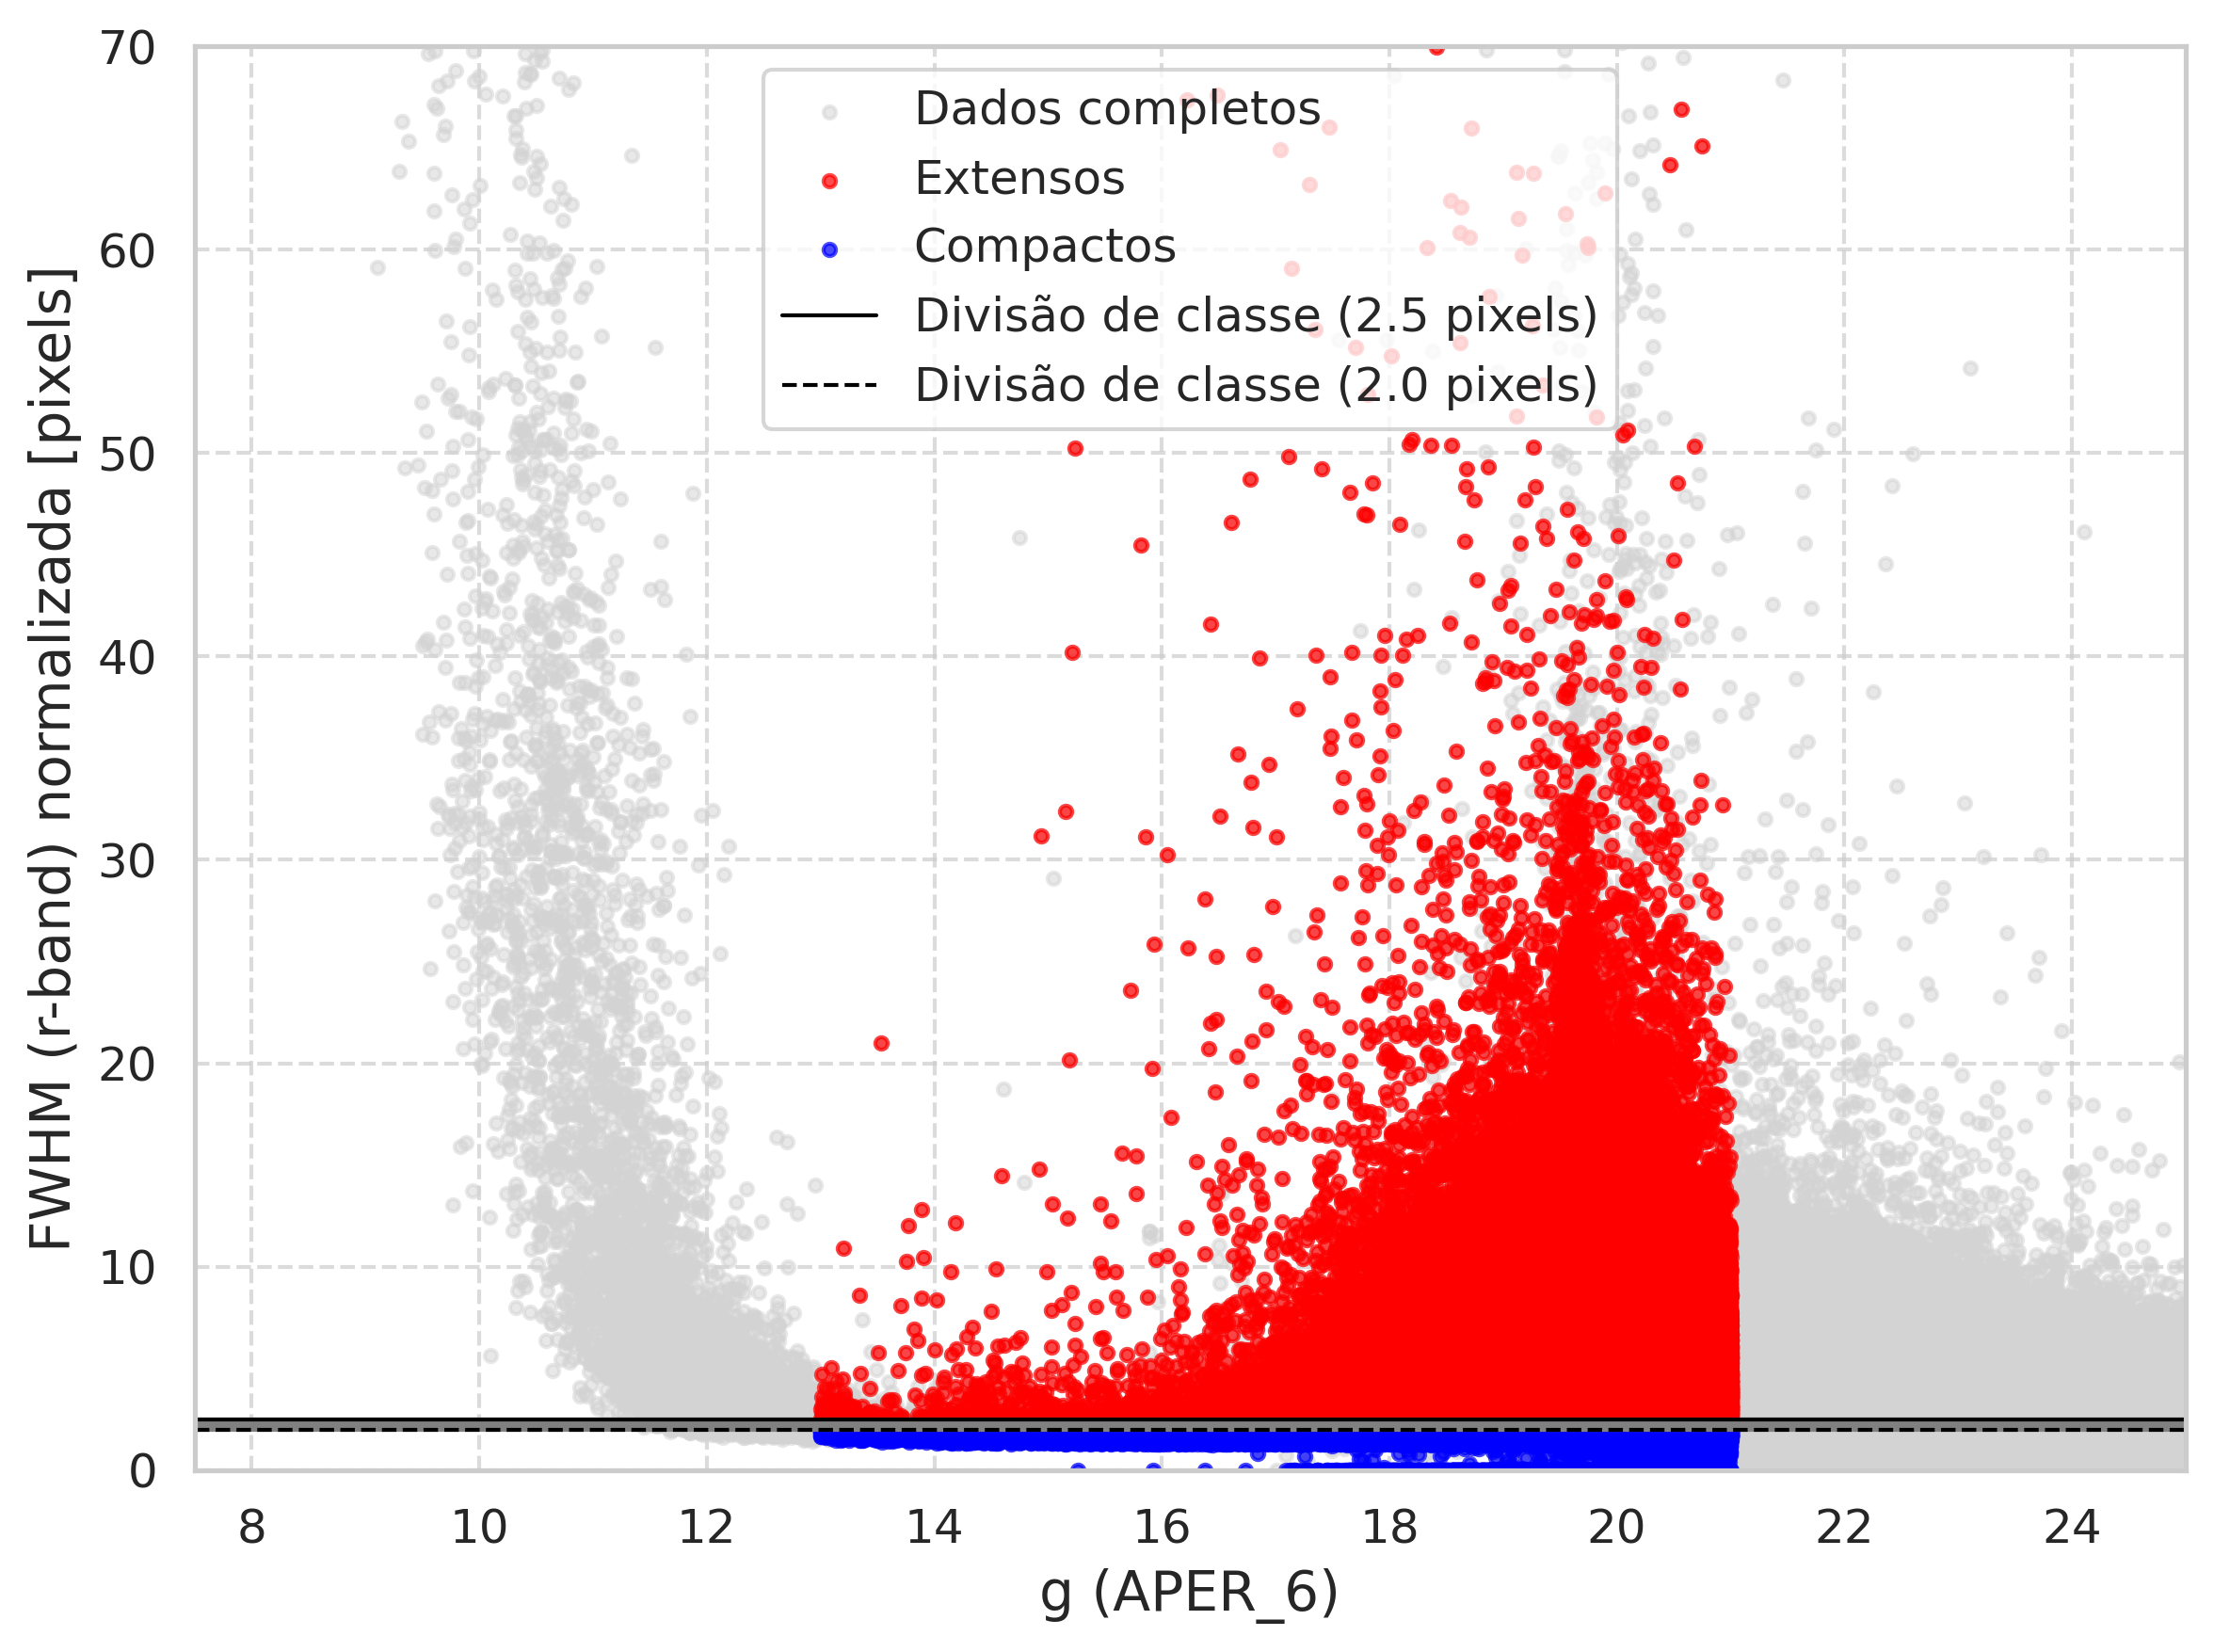
\includegraphics[width=0.85\columnwidth,angle=0]{amostra_treino.png}
    \caption[]{Distribuição da Largura Total a meia altura (\textit{FWHM} r-band) em função da magnitude \textit{g\_APER\_6} para objetos na região de Fornax, usando dados do S-PLUS Data Release 4. Objetos compactos são representados por pontos azuis, enquanto objetos extensos são indicados por pontos vermelhos. Os dados totais são mostrados em cinza. Divisão das classes: compactos (\textit{FWHM}$\leq$2 pixels) e extensos (\textit{FWHM}$\geq$2.5 pixels). Os dados entre 2 e 2.5 pixels não são usados para o treinamento do modelo, mas são mantidos na amostra de análise.}
    \label{amostra_treino}
\end{figure}

\subsection{Valores faltantes na amostra de treino}\label{subsec:valores_faltantes}
Ao preparar os dados para treinar modelos com medições do S-PLUS, decidimos alterar os valores das magnitudes na abertura APER\_6 acima de 30 para \texttt{NaN} (Not a Number). Essa decisão foi tomada para evitar que objetos com medições de baixa qualidade influenciassem o treinamento do modelo.

Na Figura \ref{missing_values_hist} temos um gráfico da fração de dados disponíveis para cada uma das bandas fotométricas.

\begin{figure}[!ht]
    \begin{center}
    % \setcaptionmargin{1cm}
    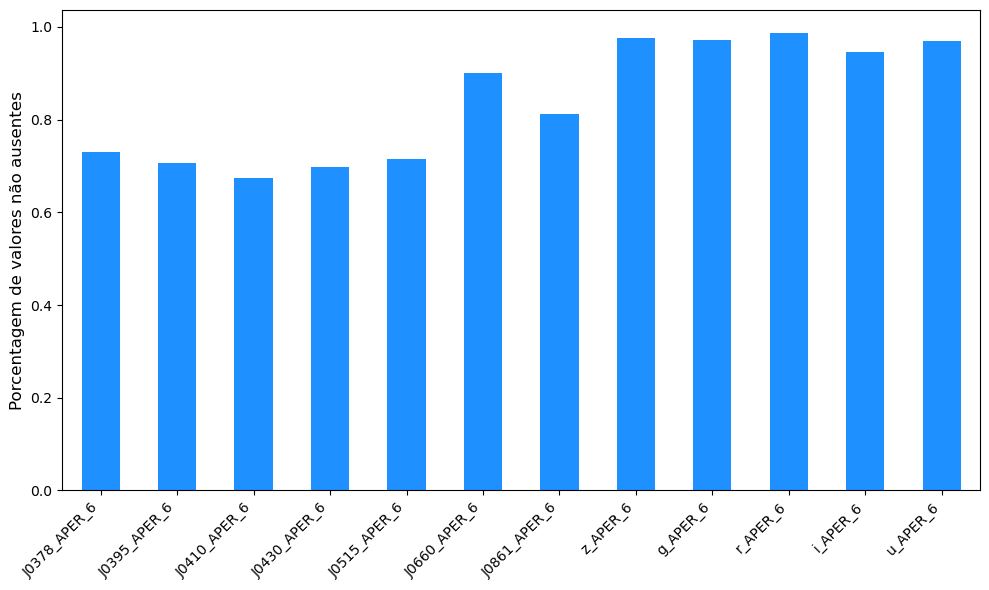
\includegraphics[width=0.8\columnwidth,angle=0]{missing_values_hist.png}
    \caption[]{Fotometria disponível em cada banda fotométrica. Cada barra representa a fração de objetos com valores disponíveis para a respectiva banda.}
    \label{missing_values_hist}
    \end{center}
\end{figure}

O gráfico mostra que a quantidade de dados ausentes varia consideravelmente entre as diferentes bandas fotométricas. A banda $u$, juntamente com algumas bandas estreitas no azul, como $J0378$, $J0395$, $J0410$ e $J0430$, apresentam a maior quantidade de valores faltantes, o que pode prejudicar a análise.

Mostramos na Figura \ref{msno_matriz} uma visualização da distribuição dos dados faltantes, onde cada linha representa um objeto e cada coluna uma banda fotométrica. As células em branco indicam valores faltantes. A Figura \ref{msno_matriz_ord} mostra a mesma matriz, mas ordenada pela magnitude $u$. Ordenamos a matriz para identificar padrões de valores faltantes que possam ser úteis para a imputação dos dados.

\begin{center}
    \begin{minipage}{0.45\textwidth}
        \centering
        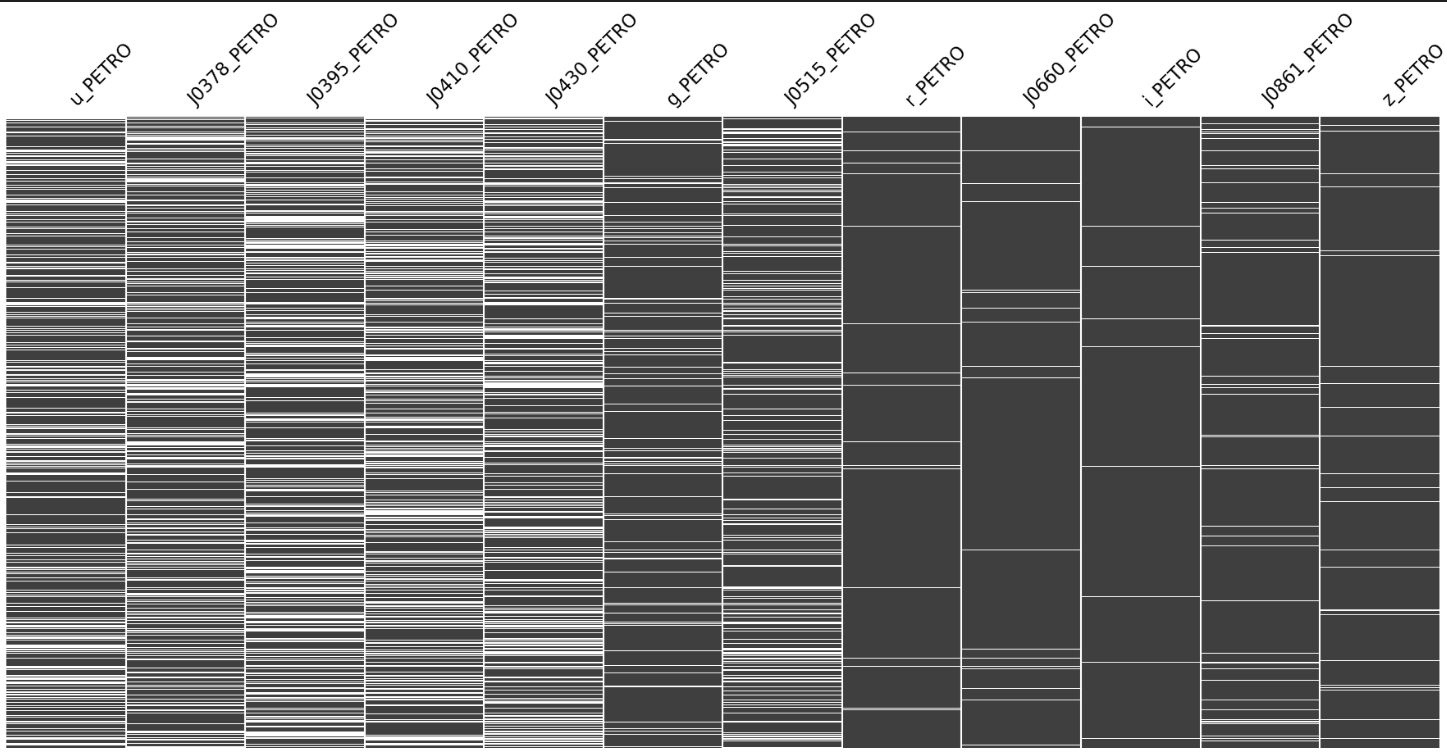
\includegraphics[width=\linewidth]{msno_matriz.png}
        \captionsetup{}
        \captionof{figure}{Distribuição de valores em cada banda fotométrica. Cada barra vertical representa as linhas da tabela original. As linhas em preto indicam objetos com valores disponíveis para a respectiva banda, enquanto os espaços em branco correspondem a linhas na tabela sem valores medidos.}
        \label{msno_matriz}
    \end{minipage}
    \hfill
    \begin{minipage}{0.45\textwidth}
        \centering
        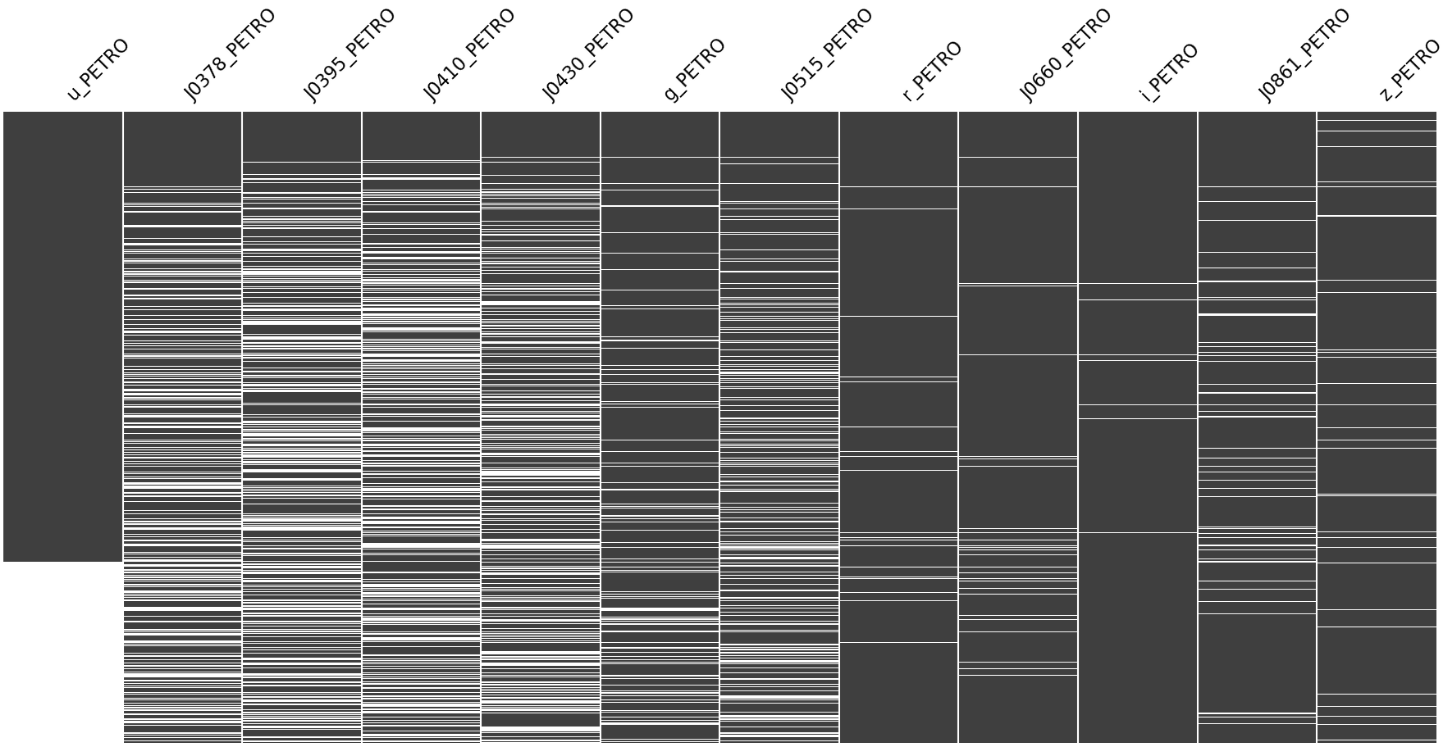
\includegraphics[width=\linewidth]{msno_matriz_ord.png}
        \captionsetup{}
        \captionof{figure}{Distribuição de valores em cada banda fotométrica, ordenada de forma que os valores disponíveis na última coluna de atributos sejam agrupados no início (coluna preenchida), enquanto os valores faltantes sejam posicionados ao final.}
        \label{msno_matriz_ord}
    \end{minipage}
\end{center}

% Uma maneira melhor de visualizar se esses valores ausentes têm alguma correlação é mostrada na Figura \ref{matriz_correlacao}, que apresenta a matriz de correlação entre os valores faltantes. Valores próximos de 1 ou -1 indicam que os valores faltantes estão, respectivamente, positivamente ou negativamente correlacionados. Valores próximos de 0 indicam que os valores faltantes são independentes.

% \begin{figure}[!ht]
%     \begin{center}
%     % \setcaptionmargin{1cm}
%     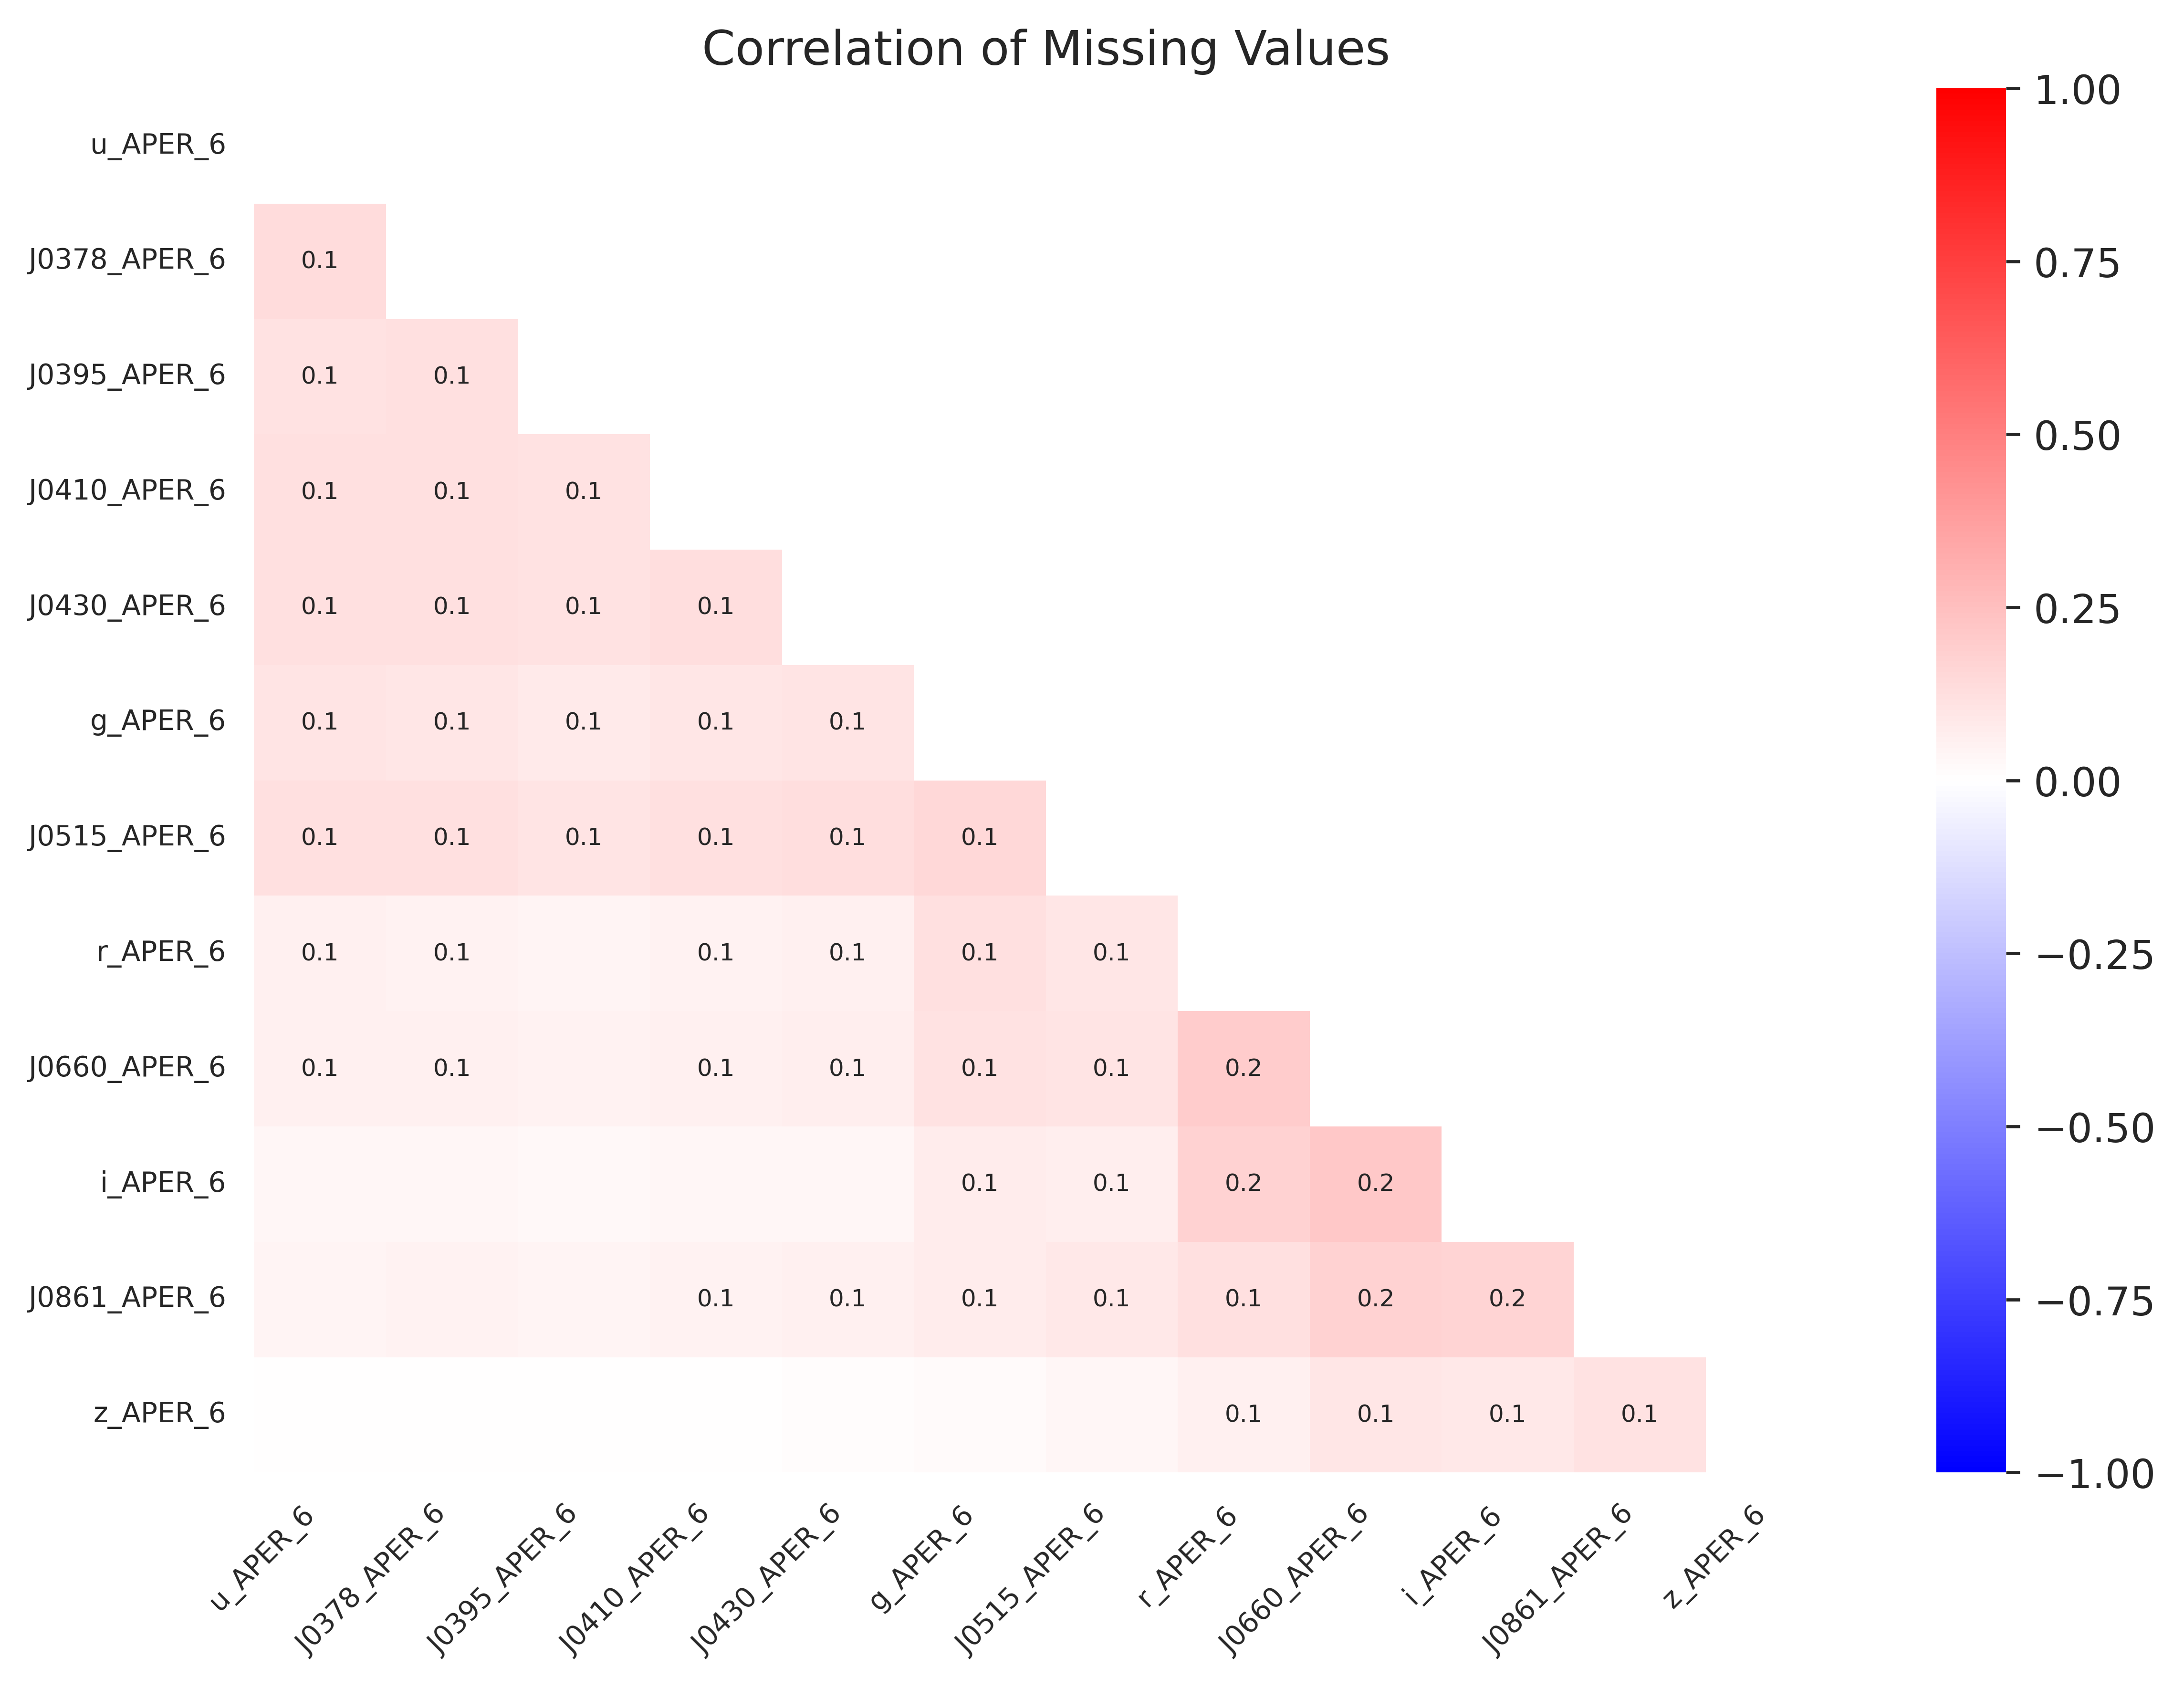
\includegraphics[width=0.85\columnwidth,angle=0]{matriz_correlacao.png}
%     \caption[]{Matriz de correlação entre os valores faltantes. Cada célula contém o coeficiente de correlação entre os valores faltantes de duas bandas fotométricas. Cores em vermelho indicam correlação positiva, enquanto cores em azul indicam correlação negativa. Valores próximos de 0 indicam que os dados faltantes são independentes.}
%     \label{matriz_correlacao}
%     \end{center}
% \end{figure}

% Pela Figura \ref{matriz_correlacao}, observamos que a maioria dos valores faltantes não apresenta correlação significativa, sugerindo que os dados faltantes são independentes.

Existem várias técnicas para lidar com esses valores ausentes. Uma maneira simples e comum é remover os objetos que possuem algum dado faltante, mas isso pode gerar uma perda de informação para o treinamento. Outra alternativa é substituir os valores faltantes pela média dos valores restantes, mas isso pode introduzir um viés na nossa seleção. Há ainda a opção de utilizar algum valor padrão, como \texttt{NaN} (Not a Number), porém, essa estratégia pode acabar confundindo o classificador, principalmente se esses valores não tiverem um significado claro para o modelo.

A técnica que adotamos para lidar com os valores faltantes foi a imputação dos dados utilizando o Método de Imputação Múltipla por Equações Encadeadas (MICE) (\citealp{MICE}). O MICE é um método de imputação que utiliza várias iterações de treinamento de modelos de aprendizado de máquina para prever os valores ausentes usando valores conhecidos de outras variáveis como preditores.

A fração de objetos da amostra, após os cortes descritos na seção \ref{subsec:cuts}, que possuem pelo menos 1, 2 ou 3 valores de magnitudes faltantes e que serão imputados, é de aproximadamente 27\%, 10\% e 3\%, respectivamente. Esses números evidenciam que uma parcela significativa dos objetos apresenta dados incompletos para as 12 magnitudes, ressaltando a importância do processo de imputação para garantir a qualidade e a consistência da análise.

\subsection{Treinando o modelo}\label{subsec:treinando_modelo}

Para o treinamento dos modelos, dividimos nossa amostra em duas classes: objetos compactos (classe 0) e objetos extensos (classe 1). Temos um total de 545.267 objetos.

Os classificadores são treinados com 80\% dos dados (436213 objetos) e testado com os 20\% restantes (109054 objetos).
% balanceado para garantir que a divisão dos dados entre treinamento e teste preserve a proporção das classes da variável. Isso significa que, se o conjunto de dados original tiver uma distribuição desbalanceada entre as classes (por exemplo, 70\% da classe 0 e 30\% da classe 1), essa mesma proporção será mantida tanto no conjunto de treino quanto no conjunto de teste. 
No conjunto de treinamento, temos 242.085 objetos classificados como pertencentes à classe 0 e 194.128 à classe 1. Já no conjunto de teste, temos 60.522 objetos da classe 0 e 48.532 da classe 1.

\raggedright
Utilizamos as 12 magnitudes da abertura APER\_6 corrigidas pela extinção (u\_APER\_6, J0378\_APER\_6, J0395\_APER\_6, J0410\_APER\_6, J0430\_APER\_6, g\_APER\_6, J0515\_APER\_6, r\_APER\_6, J0660\_APER\_6, i\_APER\_6, J0861\_APER\_6, z\_APER\_6) e as 66 combinações possíveis dessas magnitudes para formar as cores.

Os classificadores utilizados foram: \ac{KNN} e Random Forest (RF). Nos testes iniciais, tanto para o \ac{KNN} quanto para o RF, a combinação das 12 magnitudes com as 66 cores apresentou resultados superiores em comparação ao uso isolado de apenas magnitudes ou apenas cores. No caso do KNN, a melhoria foi modesta, cerca de 0,5\% nos parâmetros de desempenho (Precisão e Completeza). Já para o RF, a melhoria foi mais significativa, com um aumento médio de aproximadamente 5\% nos mesmos parâmetros. Dessa forma, optamos por utilizar a combinação de ambas as informações para o treinamento do modelo.

Os dados foram normalizados usando a amostra de treino, ajustando sua distribuição para valores entre 0 e 1, de forma a garantir a correta aplicação das métricas de distância. Para isso, utilizamos a função de normalização MinMax do \textit{sklearn} em Python, que transforma os dados para o intervalo [0, 1] com base no conjunto de treinamento. Com esse modelo de normalização salvo, reaplicamos o mesmo modelo nos dados de teste, que também serão usados para as análises posteriores.

Nas próximas subseções, discutiremos os algoritmos escolhidos para treinar nossos modelos, o processo de seleção dos melhores hiperparâmetros e a avaliação do desempenho do classificador.

\subsubsection*{K-Nearest Neighbors (KNN)}\label{subsubsec:knn}
Inicialmente, utilizamos o algoritmo K-Nearest Neighbors (KNN). O KNN é um algoritmo de aprendizado supervisionado que classifica um objeto com base em seus vizinhos mais próximos. Dada uma amostra de um conjunto de dados, ele irá calcular e avaliar as distâncias entre os objetos no espaço de parâmetros e, dada a classificação dos vizinhos mais próximos, o objeto será classificado de acordo. Para o treinamento, usamos a biblioteca \textit{scikit-learn} em Python, que implementa o algoritmo KNN.

O desempenho do KNN nos dará uma noção inicial da performance do modelo. O KNN é um algoritmo simples, mas eficaz, que pode ser utilizado como ponto de partida para a construção de modelos mais complexos. Ele é mais rápido de treinar e nos fornece uma ideia dos parâmetros que podem ser ajustados para o treinamento de modelos mais avançados.

A seleção dos melhores hiperparâmetros do modelo foi realizada por meio de uma busca com o método de \textit{GridSearchCV} da biblioteca \textit{sklearn} em Python, com validação cruzada de 5 folds (cv=5). Esse processo garantiu a otimização dos parâmetros \textit{n\_neighbors}, \textit{metric}, \textit{weights}, \textit{algorithm} maximizando o desempenho do modelo durante o treinamento.

O modelo final selecionado foi treinado com 27 vizinhos, utilizando a distância de Manhattan como métrica, pesos proporcionais à distância e \textit{algorithm}='auto'.

\subsubsection*{Random Forest (RF)}\label{subsubsec:rf}
Para o treinamento com um modelo mais robusto, utilizamos o algoritmo Random Forest (RF). O \ac{RF} é um método de aprendizado de máquina baseado em um conjunto de árvores de decisão. Durante o treinamento, o \ac{RF} constrói diversas árvores de decisão independentes, cada uma treinada com uma amostra aleatória do conjunto de dados e de seus atributos. A previsão final é obtida pela média (para regressão) ou pela votação majoritária (para classificação) das previsões individuais das árvores.

O RF é amplamente utilizado em tarefas de classificação e regressão devido à sua capacidade de lidar com dados complexos, não lineares e de alta dimensionalidade. Além disso, ele é robusto a outliers e menos suscetível ao overfitting em comparação com modelos individuais, como árvores de decisão isoladas.

Para a seleção dos hiperparâmetros do modelo RF, definimos uma grade de parâmetros para otimização, incluindo: o número de árvores na floresta (\textit{n\_estimators}), a profundidade máxima das árvores (\textit{max\_depth}), o número mínimo de amostras necessárias para dividir um nó (\textit{min\_samples\_split}), o número mínimo de amostras necessárias para formar uma folha (\textit{min\_samples\_leaf}), o uso de \textit{bootstrap} e o número de características a serem consideradas ao procurar a melhor divisão (\textit{max\_features}).

Para encontrar a melhor combinação de hiperparâmetros, dado que para o RF temos um tempo de treino consideravelmetne maior, utilizamos a biblitoeca \textit{Optuna}, do Python, para otimização de hiperparâmetros. Essa biblioteca utiliza um algoritmo de otimização bayesiana para encontrar a melhor combinação de hiperparâmetros, permitindo uma busca mais eficiente em comparação com o método de \textit{GridSearchCV}.

A melhor combinação de hiperparâmetros encontrada foi: \textit{n\_estimators}=400, \textit{max\_depth}=15, \textit{min\_samples\_split}=6, \textit{min\_samples\_leaf}=3, \textit{bootstrap}=False e \textit{max\_features}=15.



\subsection{Análise do classificador}\label{subsec:analise_modelo}
Aplicando os modelos treinados nos dados de teste, podemos realizar e avaliar as previsões feitas pelos classificador. Para comparar o desempenho dos dois modelos, utilizamos as métricas de acurácia, precisão, completeza e F1-score.

A acurácia é definida como a fração das previsões corretas em relação ao total. 

\begin{equation}
    \text{Acurácia} = \frac{TP + TN}{TP + TN + FP + FN}
\end{equation}

A precisão (ou pureza) é a fração de verdadeiros positivos em relação ao total de positivos. 

\begin{equation}
    \text{Precisão} = \frac{TP}{TP + FP}
    \label{eq:precisao}
\end{equation}

A completeza é a fração de verdadeiros positivos em relação ao total de positivos previstos.

\begin{equation}
    \text{Completeza} = \frac{TP}{TP + FN}
    \label{eq:completeza}
\end{equation}

O F1-score é a média harmônica entre precisão e completeza.

\begin{equation}
    \text{F1-score} = 2 \times \frac{\text{Precisão} \times \text{Completeza}}{\text{Precisão} + \text{Completeza}}
\end{equation}

Para ilustrar o desempenho do classificador, usamos ainda a curva AUC-ROC, amplamente utilizada para modelos de classificação binária. A ROC (Receiver Operating Characteristic) exibe a relação entre a sensibilidade (taxa de verdadeiros positivos) e a taxa de falsos positivos. A AUC (Área Sob a Curva) resume a performance em um único valor. Uma AUC de 0.5 indica classificação aleatória, enquanto 1.0 representa um modelo perfeito.

Essas são as métricas mais populares adotadas em tarefas de classificação binária. Porém, essas medidas estatísticas podem mostrar resultados excessivamente otimistas, especialmente em conjuntos de dados desbalanceados. Uma métrica adicional que usaremos é o coeficiente de correlação de Matthews (MCC), definido por:

\begin{equation}
    \text{MCC} = \frac{TP \times TN - FP \times FN}{\sqrt{(TP + FP)(TP + FN)(TN + FP)(TN + FN)}}
\end{equation}

Ela é uma métrica estatística que produz uma pontuação alta apenas se a previsão obtiver bons resultados em todas as quatro categorias da matriz de confusão, proporcionalmente tanto ao tamanho dos elementos positivos quanto ao tamanho dos elementos negativos no conjunto de dados. Os valores do MCC variam de -1 a 1, em que 1 indica uma previsão perfeita, 0 indica uma previsão aleatória e -1 indica uma previsão totalmente incorreta.

A Tabela \ref{metricas_modelo_knn} mostra as métricas obtidas no conjunto de teste para o modelo KNN treinado. Já a Tabela \ref{metricas_modelo_rf} mostra as métricas obtidas para o modelo RF treinado.

\begin{table}[!ht]
    \centering
    \caption{Classificação binária - Métricas modelo KNN}
    \begin{tabular}{lccc}
        \toprule
        Classe & Precisão & Completeza & F1-Score \\
        \midrule
        0 & 0.92 & 0.88 & 0.90 \\
        1 & 0.86 & 0.91 & 0.88 \\
        \midrule
        \multicolumn{3}{l}{AUC-ROC} & 0.95 \\
        \multicolumn{3}{l}{Coeficiente de Correlação de Matthews (MCC)} & 0.78 \\
        \bottomrule
    \end{tabular}
    \label{metricas_modelo_knn}
\end{table}


\begin{table}[!ht]
    \centering
    \caption{Classificação binária - Métricas modelo RF}
    \begin{tabular}{lccc}
        \toprule
        Classe & Precisão & Completeza & F1-Score \\
        \midrule
        0 & 0.95 & 0.90 & 0.92 \\
        1 & 0.89 & 0.94 & 0.91 \\
        \midrule
        \multicolumn{3}{l}{AUC-ROC} & 0.97 \\
        \multicolumn{3}{l}{Coeficiente de Correlação de Matthews (MCC)} & 0.84 \\
        \bottomrule
    \end{tabular}
    \label{metricas_modelo_rf}
\end{table}

Na Figura \ref{confusion_matrix}, temos a matriz de confusão dos modelos, mostrando a quantidade de verdadeiros positivos (TP), verdadeiros negativos (TN), falsos positivos (FP) e falsos negativos (FN) obtidos.

\begin{figure}[!ht]
    \centering
    \captionsetup{justification=centering}
    \begin{subfigure}[b]{0.45\textwidth}
        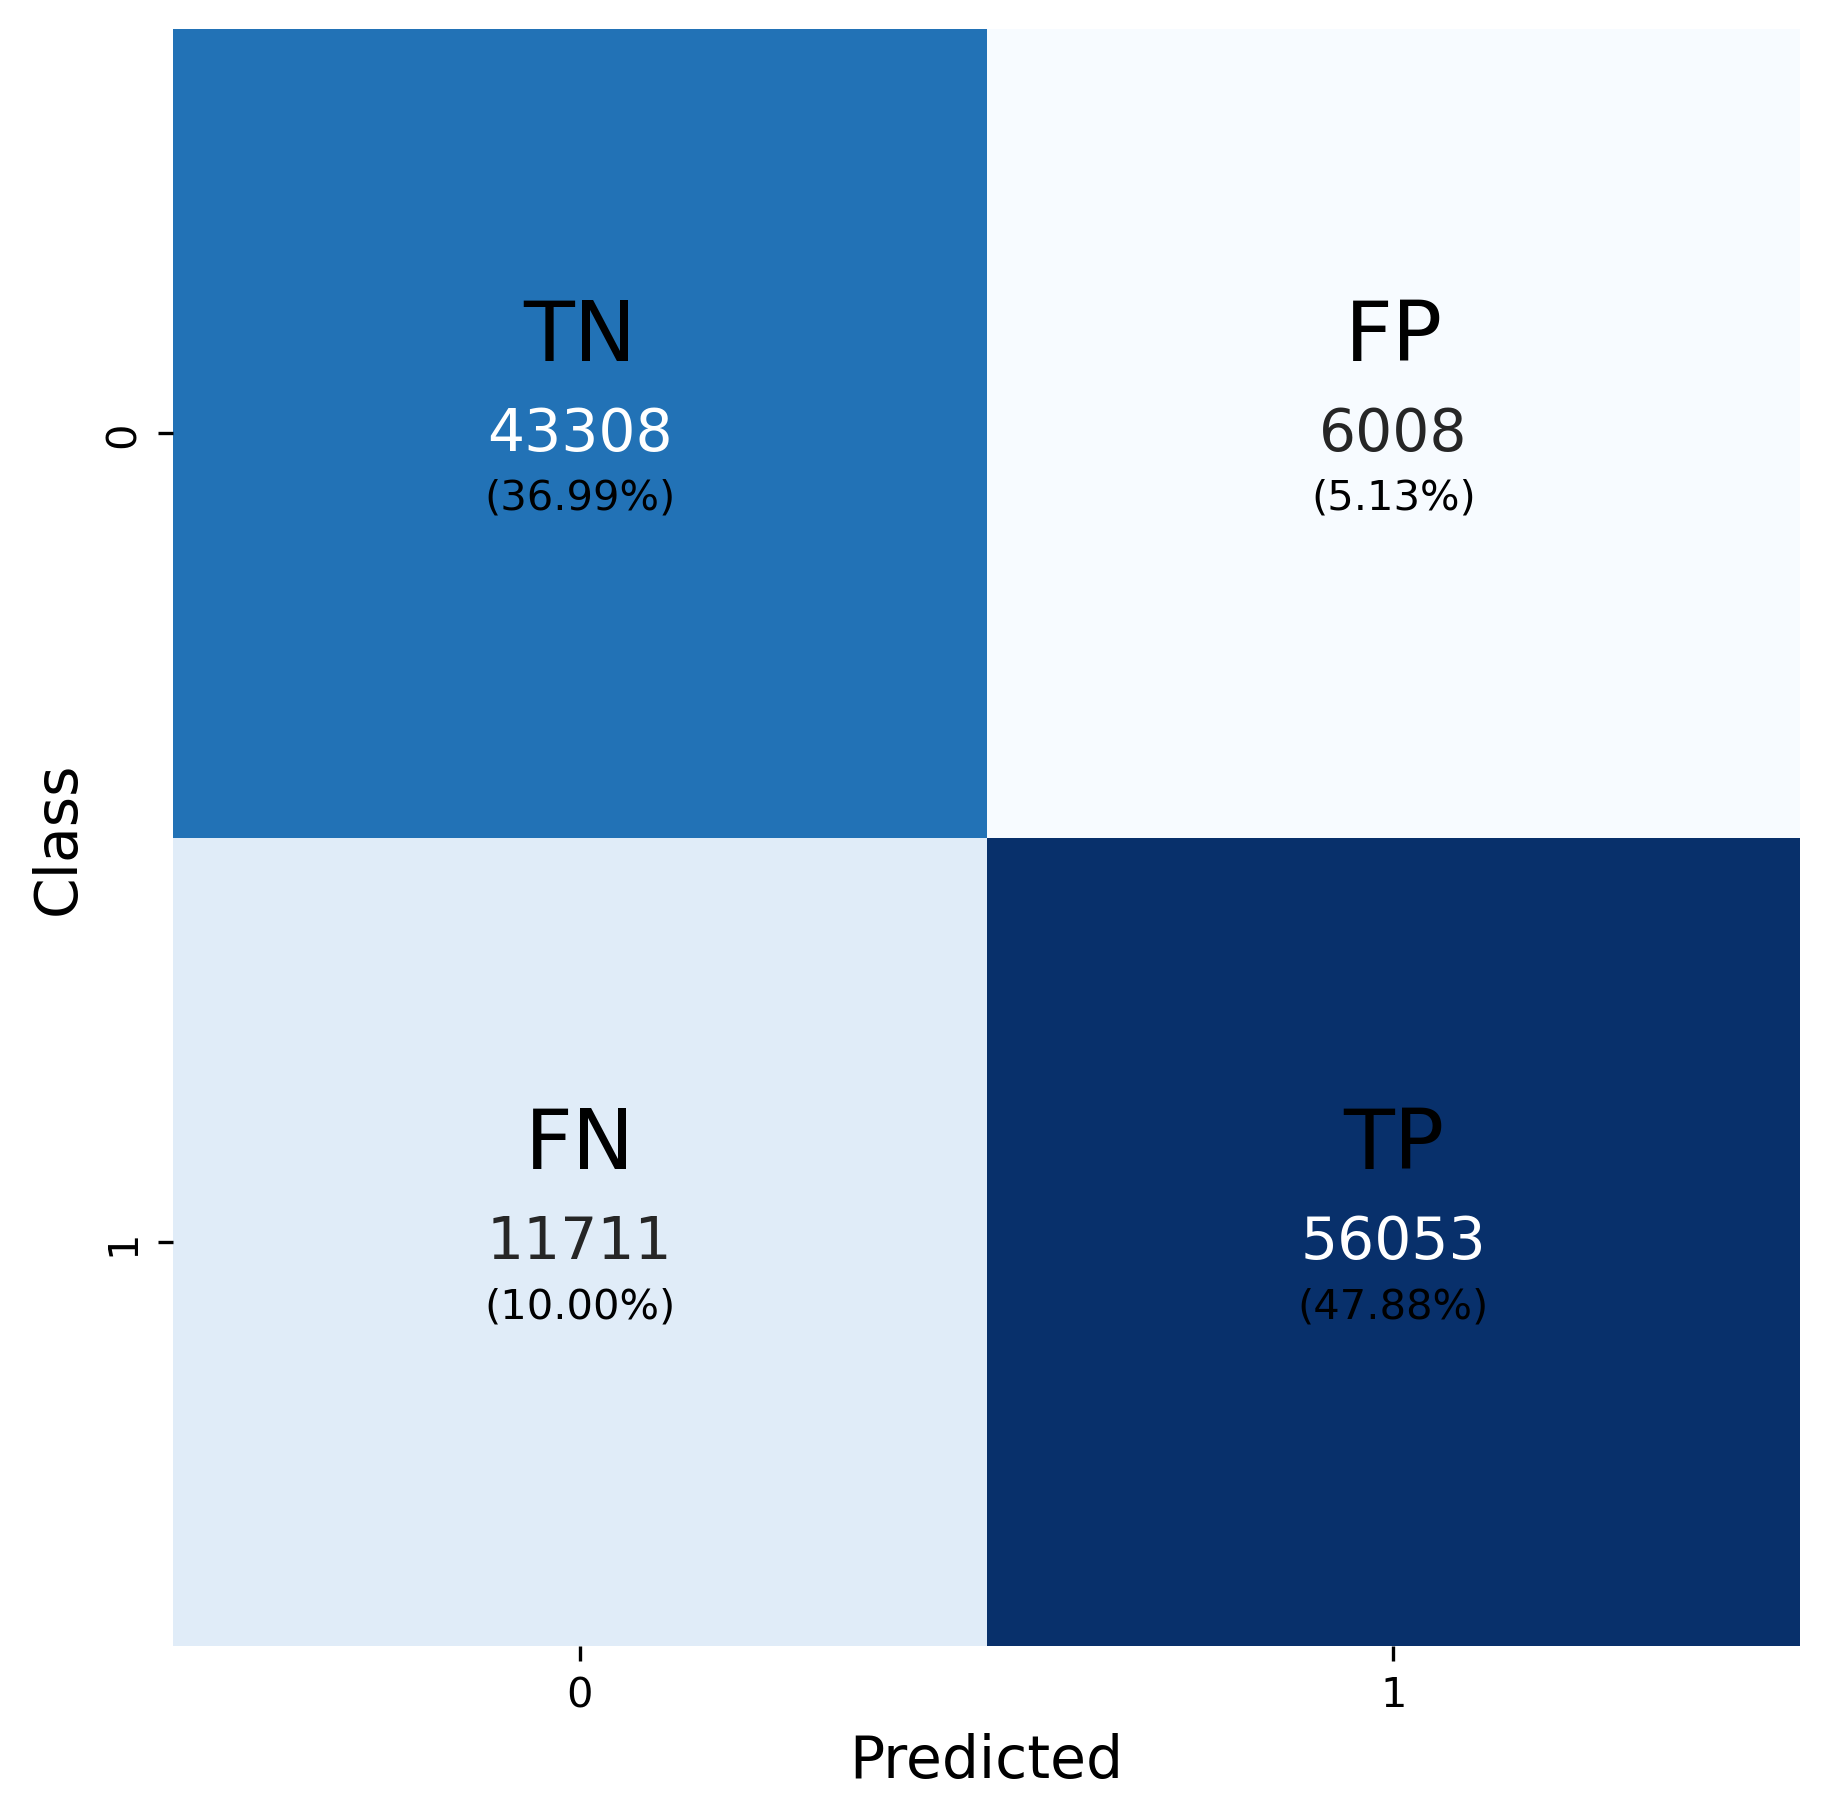
\includegraphics[width=\textwidth]{confusion_matrix_knn.png}
        \caption{Modelo KNN}
    \end{subfigure}
    \begin{subfigure}[b]{0.45\textwidth}
        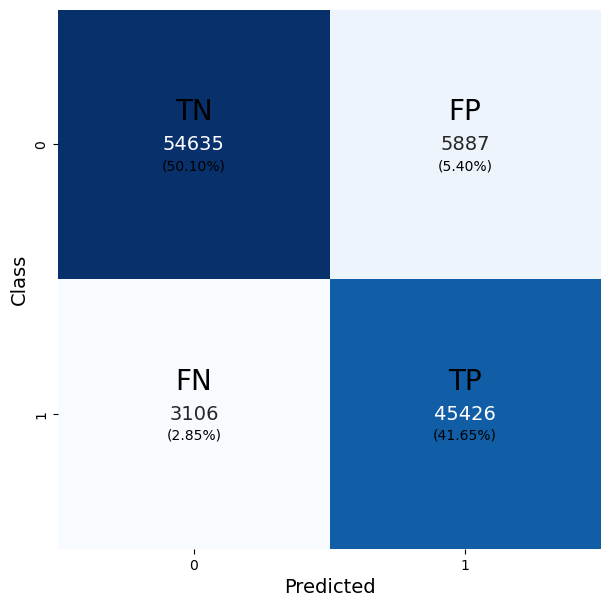
\includegraphics[width=\textwidth]{confusion_matrix_rf.png}
        \caption{Modelo RF}
    \end{subfigure}
    \caption{Matriz de confusão do modelo KNN (a) e do modelo RF (b). A diagonal principal representa os valores corretamente classificados, enquanto os valores fora da diagonal principal representam os erros de classificação das classes 0 e 1.}
    \label{confusion_matrix}
\end{figure}

Pelos resultados das métricas adotadas, e também pela matrizes de confusão, podemos observar que o modelo RF apresenta um desempenho superior ao modelo KNN. Assim, optamos por utilizar o modelo RF para a classificação dos objetos compactos e extensos.

Muitos dos objetos tiveram classificação correta, como podemos ver na diagonal principal das matrizes de confusão da Figura \ref{confusion_matrix}. Porém, cabe ressaltar que nem todos os objetos do conjunto de teste eram estrelas ou galáxias, mas sim, majoritariamente, mais de cada um deles nas classes de compactos e extensos, respectivamente. Assim, é esperado que algumas classificações sejam feitas de forma errada, e é nessa proposta que o modelo foi treinado: encontrar aqueles com maior probabilidade de serem extensos, mas que fazem parte do conjunto dos compactos.

Os resultados obtidos pelo RF têm valores de precisão, completeza e F1-score acima de 0,89 para ambas as classes. A AUC-ROC de 0,97 indica que o modelo é capaz de distinguir entre as duas classes com boa precisão, dadas as limitações dos conjuntos de treinamento. O coeficiente de correlação de Matthews (MCC) de 0,84 é um indicativo de que o modelo é capaz de prever corretamente a maioria dos objetos.

Foram realizadas as previsões de probabilidade de ser da classe 1 (objetos extensos) para toda a amostra que estaremos analisando na busca (amostra de treino e amostra de teste). A Figura \ref{probabilidade_extensos_fwhm} mostra, para o KNN, a distribuição de \textit{FWHM} na banda \textit{r} dos objetos com classificação como estrela ou galáxia do GAIA DR3 com probabilidade maior que 90\%. Sobreposta na imagem, temos matrizes de confusão do classificador para diferentes intervalos de \textit{FWHM}.

\begin{figure}[!ht]
    \centering
    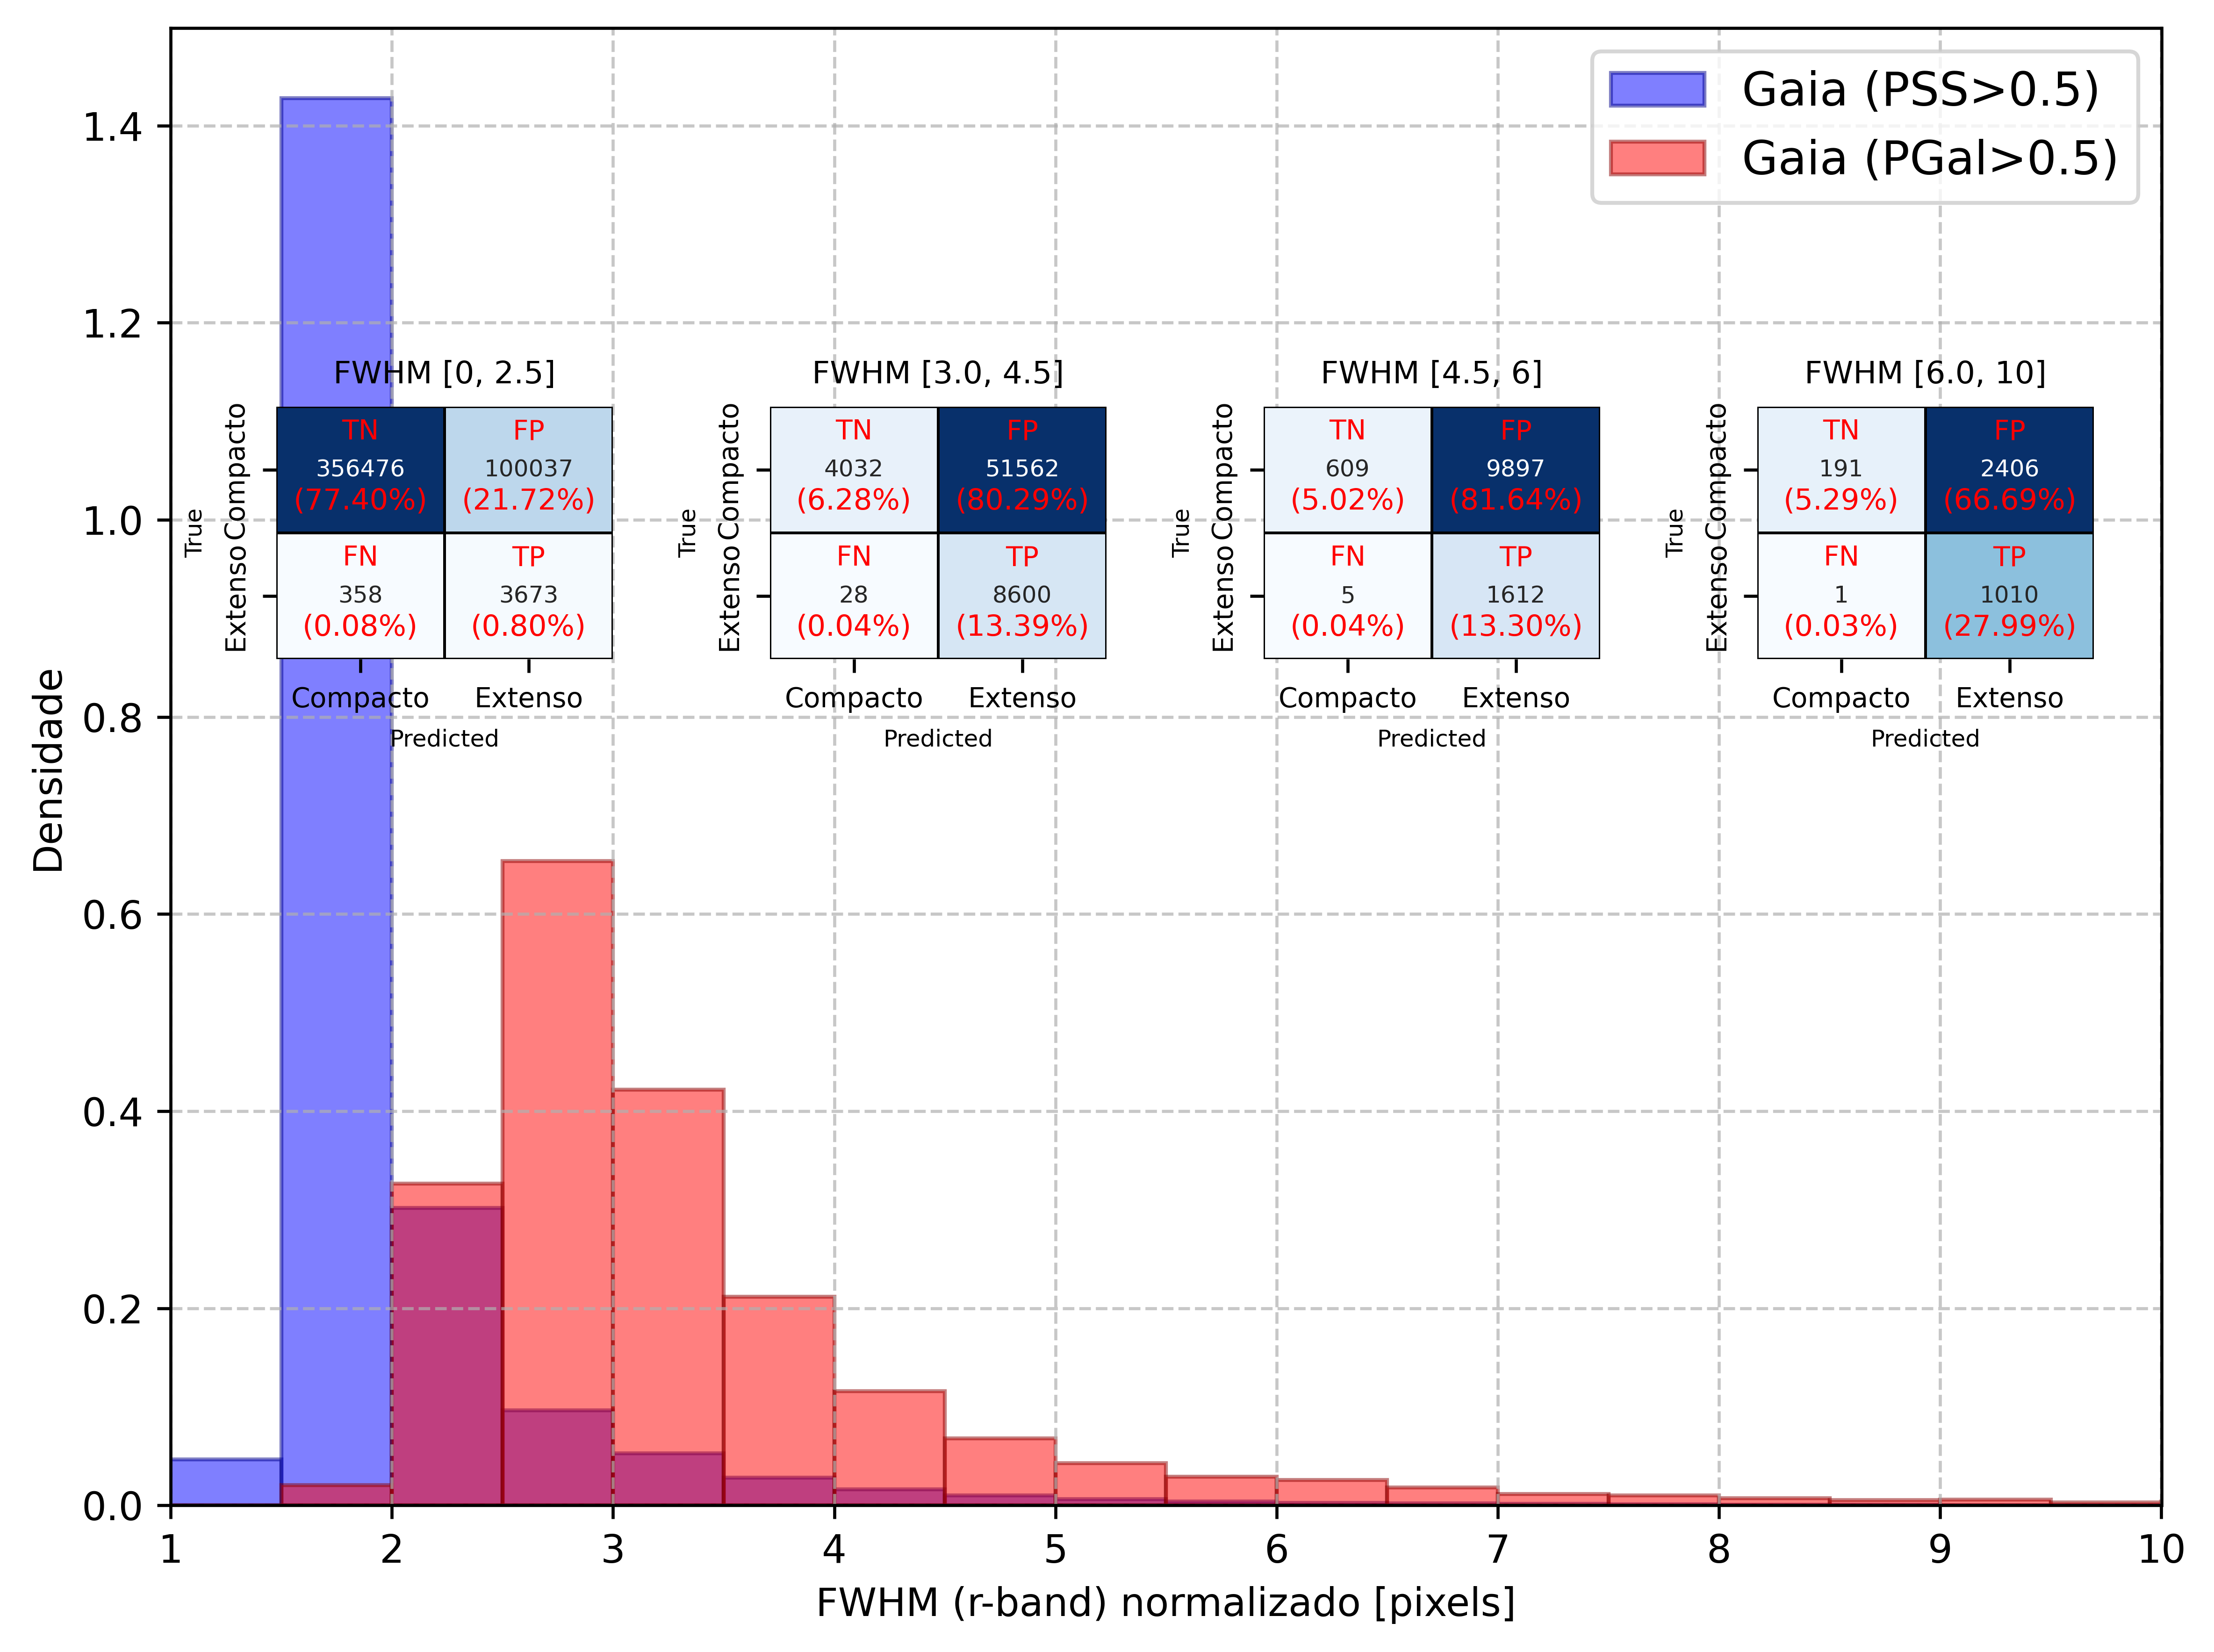
\includegraphics[width=1.\columnwidth,angle=0]{distribution_of_stars_and_galaxies_with_cm.png}
    \caption[]{Distribuição de \textit{FWHM (r-band)} para objetos da amostra com classificação estrela-galáxia do GAIA DR3 com probabilidade maior que 90\%. As matrizes de confusão do classificador RF para diferentes intervalos de \textit{FWHM} estão sobrepostas. O classificador dá a probabilidade de ser da classe 1 (extensos) para cada objeto. }
    \label{probabilidade_extensos_fwhm}
\end{figure}

O comportamento do classificador nas matrizes de confusão mostra que, para as regiões de \textit{FWHM} menores (entre [0, 2.5]), onde há uma maior concentração de estrelas, observa-se uma alta taxa de classificação para objetos do tipo compacto. Já para objetos com \textit{FWHM} maiores, o classificador mostra uma tendência de classificá-los como extensos, o que é esperado, já que esses objetos são menos prováveis de serem estrelas. Para objetos com \textit{FWHM} nas faixas de sobreposição, o desempenho do classificador é misto, refletindo a dificuldade em separar essas classes na região. Porém, é possível observar uma transição gradual entre as classes, consistente com os picos das distribuições de \textit{FWHM}.

Ilustrando ainda o resultado da classificação, apresentamos na Figura \ref{predic_colored} o mesmo gráfico da Figura \ref{amostra_treino} para os objetos da amostra de teste, coloridos de acordo com a probabilidade de serem objetos extensos pelo modelo RF. A cor azul indica uma probabilidade baixa, enquanto a cor vermelha indica uma probabilidade alta. 

Do classificador para a amostra, tivemos um total de 1.803.561 objetos analisados, dos quais 1.411.903 (78,28\%) apresentaram probabilidade acima de 50\% de serem extensos, enquanto 391.658 (21,72\%) apresentaram probabilidade abaixo de 50\%. Entre os objetos com probabilidade acima de 50\% de serem extensos, 311.846 (17,29\%) possuem \textit{FWHM} menor que 2,5 pixels, ou seja, são objetos compactos que têm mais de 50\% de chance de serem semelhantes à amostra de objetos extensos.

\begin{figure}[!ht]
    \centering
    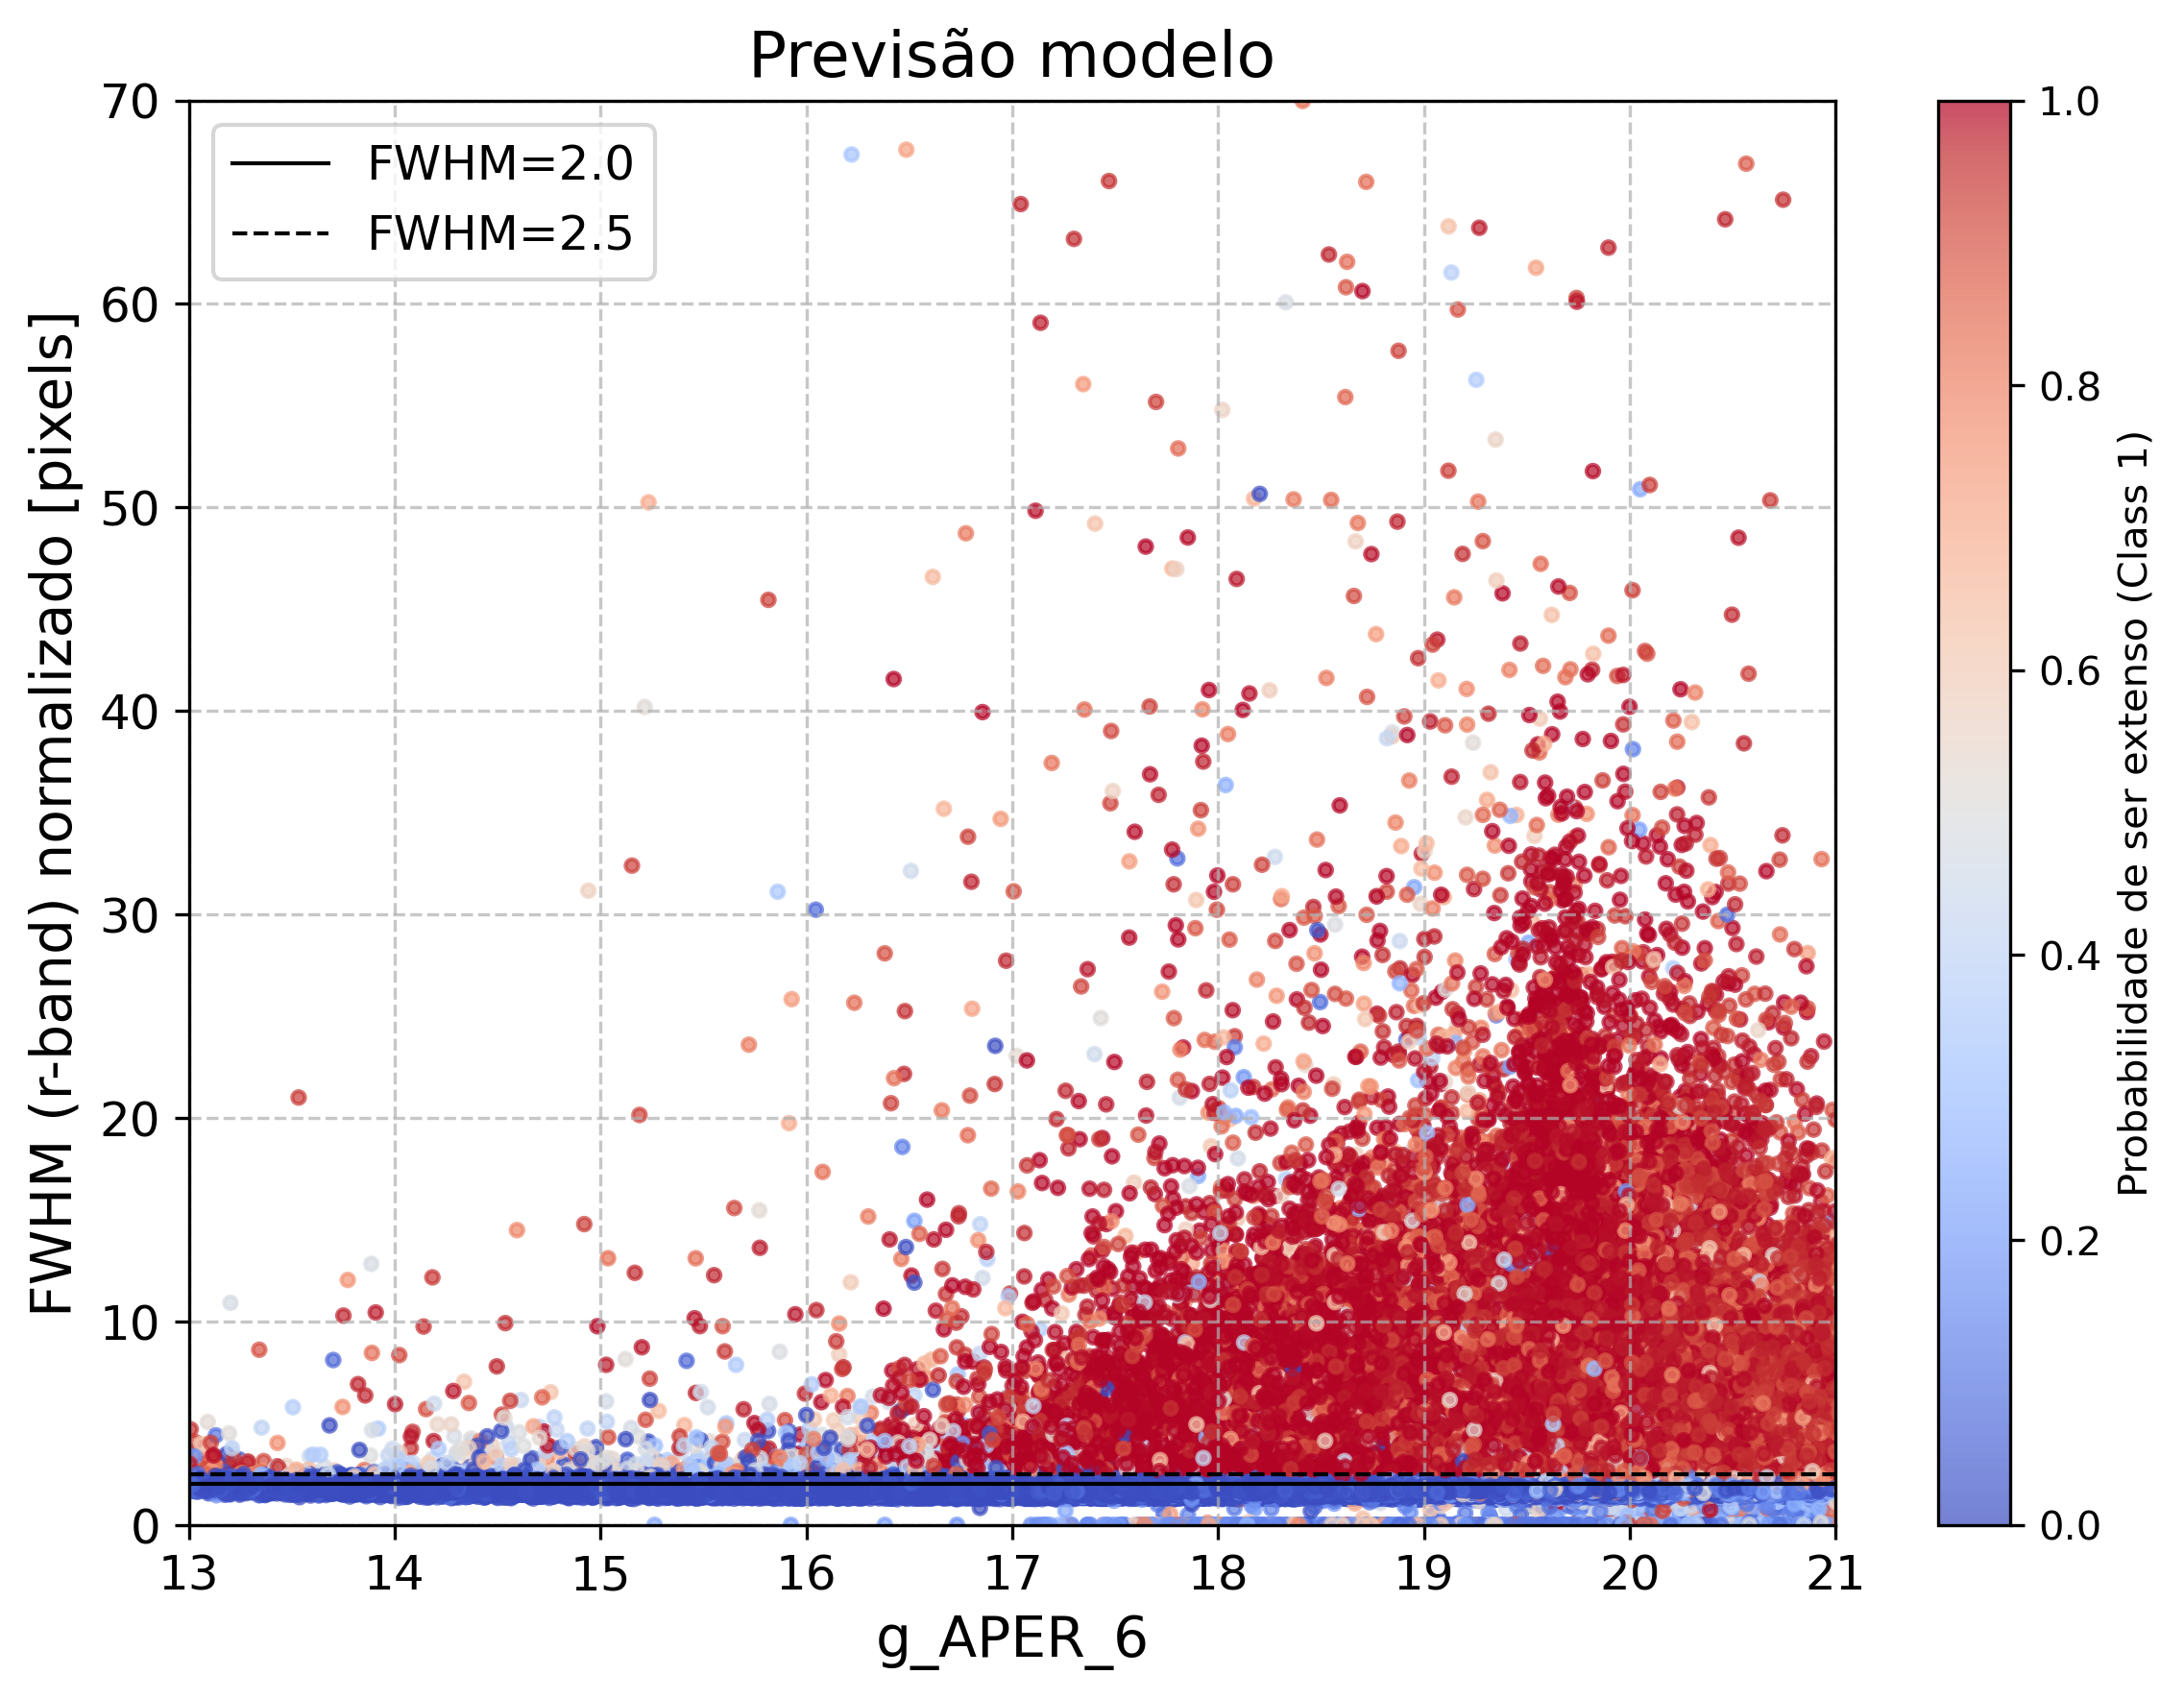
\includegraphics[width=1.\columnwidth,angle=0]{predic_colored.png}
    \caption[]{Distribuição da Largura Total na Metade Máxima (\textit{FWHM} r-band) em função da magnitude \textit{g\_APER\_6} para objetos da amostra de teste, coloridos de acordo com a probabilidade de serem objetos extensos (Classe 1) pelo modelo. Divisão das classes: compactos (\textit{FWHM}$\leq$2 pixels) e extensos (\textit{FWHM}$\geq$2.5 pixels).}
    \label{predic_colored}
\end{figure}

A probabilidade dos objetos serem da classe 1 (objetos extensos) para as UCDs conhecidas na amostra é apresentada na Tabela \ref{ucds_predict}.

\begin{table}[H]
    \centering
    \caption{Classificação do modelo para a classe 1 (objetos extensos) das UCDs na amostra de análise}  
    \begin{tabular}{lc}
        \toprule
        Nome & Predição modelo RF \\
        \midrule
        UCD3 & 0.36 \\
        UCD1 & 0.98 \\
        F-24 & 0.99 \\
        UCD5 & 0.38 \\
        F-1a & 0.11 \\
        F-9 & 0.87 \\
        F-5 & 0.53 \\
        F-6 & 0.89 \\
        F-7 & 0.70 \\
        F-12 & 0.73 \\
        F-11 & 0.97 \\
        F-34 & 0.98 \\
        F-22 & 0.93 \\
        % F-53 & 0.96 \\
        % F-51 & 0.96 \\
        % F-59 & 0.92 \\
        \bottomrule
    \end{tabular}
    \label{ucds_predict}
\end{table}

Das 13 UCDs presentes, 9 foram classificadas com uma predição acima de 70\%, e 2 com classificação muito pouco provável. 

% \subsection*{Previsões para aglomerados globulares}\label{subsec:predicoes_gc}


% Como mencionado neste trabalho, parte das UCDs estudadas possivelmente têm sua formação associada a aglomerados globulares (Globular Clusters, GCs). A classificação adotada para distinguir UCDs de GCs, conforme descrito na seção \ref{subsec:cuts}, considera objetos com \textit{g}$\leq$21 como UCDs e aqueles com \textit{g}$>$21 como GCs.

% Para o classificador RF, podemos obejtsar o seu comportamento e classiicação para GCs na nossa amostra. Para Uma lsita de GCs em Fornax, usmaos os dados vindo de \cite{Saifollahi_2021}, que apresenta uma lista de GCs/UCDs conhecidas na região de Fornax. Removemos 

\section{Redshifts fotométricos}\label{sec:zphot}

A determinação de redshifts é uma etapa importante para identificar a localização dos objetos no universo. Nesse trabalho, os \ac{photoz} (\textit{$z_{phot}$}) permitem que estimemos a distância dos objetos de forma eficiente e em larga escala, utilizando apenas dados fotométricos. Essa abordagem é especialmente útil quando não há disponibilidade de redshifts espectroscópicos (\textit{$z_{spec}$}). A utilização de redshifts fotométricos têm o objetivo de filtrar objetos que não pertencem ao aglomerado de Fornax, reduzindo a contaminação por objetos de fundo.

É possível encontrar redshifts fotométricos para parte dos objetos da nossa amostra em outros trabalhos da literatura, assim como em catálogos da própria colaboração S-PLUS \citep{erik_photoz_2024}. Porém, para a busca neste projeto, utilizamos dados com a redução da fotometria do S-PLUS diferentes dos utilizados para os \textit{$z_{phot}$} disponíveis. Assim, mesmo que vindos do mesmo catálogo, uma pequena parte dos objetos na nossa amostra não tem redshifts fotométricos disponíveis. Dos 2900926 objetos iniciais da nossa amostra, 290637 objetos não têm redshifts fotométricos disponíveis em \citep{erik_photoz_2024}.

Abordagens comuns para a estimativa de \textit{$z_{phot}$} incluem o ajuste baseado em modelos espectrais (\textit{template fitting}) e técnicas de aprendizado de máquina. O método de \textit{template fitting} apresenta a vantagem de permitir extrapolações, sendo útil para objetos cujas propriedades não estão bem representadas em amostras conhecidas (e.g., \citealt{Bolzonella_2000}; \citealt{Gorecki_2014}). Já o aprendizado de máquina tende a ser mais eficiente e preciso quando treinado com um conjunto de dados representativo, embora sua capacidade de generalização seja limitada fora do intervalo coberto pelo treinamento (e.g., \citealt{Carrasco_2013}; \citealt{Sadeh_2016}). Além disso, algoritmos de aprendizado de máquina costumam oferecer tempos de inferência mais rápidos, o que os torna especialmente atrativos em contextos com grandes volumes de dados.


Aqui optamos por utilizar o método de aprendizado de máquina para calcular \textit{$z_{phot}$}. Para isso, empregamos modelos de regressão utilizando o algoritmo Random Forest (RF), implementado em Python. No caso da regressão, o RF cria uma floresta de árvores de decisão, onde cada uma delas é treinada com uma amostra aleatória do conjunto inicial dos dados e de seus atributos. A previsão para o valor de \textit{$z_{phot}$} é feita pela média das previsões de cada árvore.

Para a seleção da amostra de treino, utilizamos o mesmo catálogo de Fornax usado anteriormente, com os dados de fotometria do S-PLUS provenientes de \cite{haack2024splusfornaxprojectsfp} (\textit{Run 1}). Ou seja, temos os mesmos dados descritos na seção \ref{sec:Fornax_data}, com as 12 magnitudes corrigidas pela extinção (como descrito na seção \ref{sec:Coeficientes_ext}).

Dessa amostra, selecionamos os objetos com redshifts espectroscópicos disponíveis, provenientes do catálogo \cite{Lima_2024}. Selecionamos os objetos em um intervalo de redshifts entre 0.002 até 0.5, dessa maneira evitamos boa parte das estrelas (com redshifts menores) e galáxias muito distantes de Fornax. Adotamos um intervalo de magnitude de 15$\leq$\textit{r\_APER\_6}$\leq$21, evitando objetos muito brilhantes e saturados, e objetos com baixa qualidade de medição.

Removemos também os objetos com medições faltantes em alguma das 12 magnitudes das aberturas \textit{APER\_6}, resultando em uma amostra final com 12.296 objetos.

Para o treinamento, os melhores resultados a princípio se deram com a utilização das combinações das 66 cores das 12 magnitudes de abertura \textit{APER\_6}. Assim, treinamos o modelo fornecendo o redshift espectroscópico (\textit{$z_{spec}$}) como variável alvo e as 66 cores como variáveis preditoras.

Dividimos a amostra em 80\% para treino e 20\% para teste. O conjunto de dados foi normalizado usando a amostra de treino, ajustando sua distribuição para valores entre 0 e 1 pela função MinMax do Python. 

A Figura \ref{zphot_zspec} mostra a comparação entre os redshifts espectroscópicos (\textit{$z_{spec}$}) e fotométricos (\textit{$z_{phot}$}) para a amostra de treino. A linha tracejada representa a relação 1:1 entre os redshifts, enquanto a linha contínua representa a relação ajustada pelo modelo de regressão.

\begin{figure}[!ht]
    \centering
    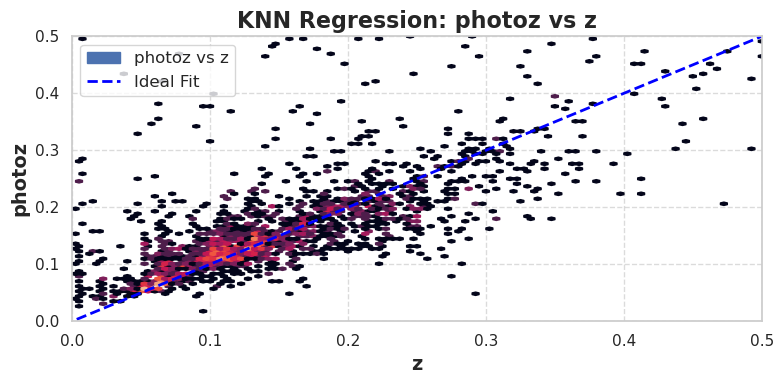
\includegraphics[width=1.\columnwidth,angle=0]{zphot_zspec.png}
    \caption[]{Resultados da regressão com o algoritmo Random Forest (RF) para estimar os redshifts fotométricos (\textit{$z_{phot}$}) em relação aos redshifts espectroscópicos (\textit{$z_{spec}$}). Na parte superior, o gráfico de dispersão compara \textit{$z_{phot}$} vs \textit{$z_{spec}$}. A linha azul tracejada representa o ajuste ideal (\textit{$z_{phot}$} = \textit{$z_{spec}$}). A densidade de pontos é representada por um gradiente de cores, com áreas mais densas indicadas em tons mais claros.}
    \label{zphot_zspec}
\end{figure}

Percebemos pela Figura \ref{zphot_zspec} que o modelo de regressão foi capaz de estimar os redshifts fotométricos com certa precisão. As métricas que adotamos para avaliar o desempenho do modelo foram o erro quadrático médio (EQM), o $R^2$, o $\sigma_{nmad}$ e a fração de outliers (Fout). O EQM é uma medida da média dos erros quadráticos entre os valores previstos e os valores reais. O $R^2$ é uma medida de quão bem os dados se ajustam ao modelo, variando de 0 a 1, onde 1 indica um ajuste perfeito. O $\sigma_{nmad}$ é uma medida robusta de dispersão que quantifica a variação dos resíduos em relação à mediana. 

% A fração de outliers (Fout) é a proporção de previsões que estão além de um certo limite em relação aos valores reais. Um critério comum é considerar como outliers os casos em que:

% [ \left| \frac{z_{phot} - z_{spec}}{1 + z_{spec}} \right| > 0.15 ]

Os resultados obtidos para essas métricas foram: EQM = 0,05, $R^2$ = 0,6, $\sigma_{nmad}$ = 0,03. Embora os valores indiquem uma precisão moderada, o modelo apresenta algumas estimativas com erros maiores, especialmente para redshifts mais elevados. É importante destacar que o objetivo principal deste modelo não é fornecer redshifts altamente precisos para todos os objetos, mas sim identificar aqueles com redshifts compatíveis com o aglomerado de Fornax. Dessa forma, mesmo com a presença de erros, o modelo é útil para filtrar objetos com maior probabilidade de pertencerem ao fundo, proporcionando um ganho significativo na seleção de candidatos.

Aplicando o modelo para as UCDs conhecidas em Fornax, obtivemos os resultados apresentados na Tabela \ref{ucds_zphot}, juntamente com os redshifts fotométricos fornecidos por \cite{erik_photoz_2024} (\textit{zml}). Para os objetos que possuem redshifts fotométricos disponíveis em \citep{erik_photoz_2024}, observamos que esses valores são mais precisos e compatíveis com os esperados para Fornax, em comparação com os redshifts fotométricos estimados pelo nosso modelo.

Essa diferença de desempenho é compreensível, dado que o modelo de \cite{erik_photoz_2024} utiliza uma abordagem mais robusta, baseada em uma amostra maior de objetos com redshifts espectroscópicos conhecidos e é treinado com um número superior de dados, o que proporciona maior confiabilidade nos resultados. Por outro lado, nosso modelo, embora tenha apresentado resultados razoáveis, é limitado pela menor quantidade de dados disponíveis para o treinamento.

Portanto, concluímos que, sempre que possível, os cortes baseados em redshifts fotométricos devem ser realizados utilizando os valores de \cite{erik_photoz_2024}. Para os casos em que esses dados não estão disponíveis, utilizaremos os redshifts fotométricos estimados pelo nosso modelo como uma alternativa, cientes de suas limitações.

\begin{table}[!ht]
    \centering
    \caption{Aplicação do modelo de regressão para estimativas de redshifts fotométricos para UCDs conhecidas na amostra de análise de Fornax (\textit{$z_{phot}$}), junto com as previsões de \citep{erik_photoz_2024} (\textit{zml}), para aqueles objetos que tinham dados presentes e o redshift espectroscópico (\textit{$z_{spec}$}) disponível.}
    \begin{tabular}{lccc}
        \toprule
        Nome & \textit{$z_{phot}$} & \textit{zml} & \textit{$z_{spec}$}\\
        \midrule
        UCD3 & 0.07 & 0.03 & 0.0053\\
        UCD1 & 0.09 & 0.08 & 0.0052\\
        F-24 & 0.08 & 0.04 & 0.0062\\
        UCD5 & 0.03 & 0.04 & 0.0045\\
        F-1a & 0.21 & -- & 0.0042\\
        F-9 & 0.09 & 0.07 & 0.0058\\
        F-5 & 0.06 & -- & 0.0057\\
        F-6 & 0.10 & -- & 0.0037\\
        F-7 & 0.19 & 0.16 & 0.0050\\
        F-12 & 0.07 & -- & 0.0055\\
        F-11 & 0.10 & -- & 0.0059\\
        F-34 & 0.07 & -- & 0.0054\\ 
        F-22 & 0.09 & 0.06 & 0.0034\\
        F-53 & 0.31 & -- & 0.0020\\
        F-51 & 0.10 & -- & 0.0041\\
        F-59 & 0.06 & -- & 0.0060\\
        \midrule
    \end{tabular}
    \label{ucds_zphot}
\end{table}

Tanto pela Figura \ref{zphot_zspec} quanto pela Tabela \ref{ucds_zphot}, podemos observar que o modelo de regressão superestima os redshifts fotométricos para objetos com redshifts mais baixos como de Fornax. Porém nosso objetivo não é estimar redshifts precisos para todos os objetos, mas sim aplicar um corte que nos ajude a remover objetos com maiores chances de serem do fundo.

Sabendo que o redshift de Fornax é de aproximadamente $0.005$\footnote{https://simbad.u-strasbg.fr/simbad/sim-id?Ident=Fornax+Cluster}, e observando os redshifts fotométricos estimados para as UCDs conhecidas, podemos adotar um corte conservador para os redshifts fotométricos, com uma margem otimista para o erro.

\section{Seleção das candidatas}\label{sec:selecao_candidatas}
Para a seleção das candidatas, queremos primeiramente criar uma subamostra dos dados de Fornax, contendo os objetos compactos de nosso interesse. A partir dessa amostra, iremos selecionar pelas probabilidades de serem extensos (classe 1). Para amostra inicial, depois dos cortes feitos da seção \ref{subsec:cuts}, temos um total de 1.803.561 objetos com as predições do classificador. 

A partir de \cite{Su_2021}, removemos os objetos confirmados espectroscopicamente como sendo do background. Usando o catálogo de redshifts espectroscópicos de \cite{Lima_2024}, removemos os objetos que possuem redshifts maiores que 0.0055, considerando que esses objetos estão mais distantes de Fornax e, portanto, não pertencem ao aglomerado. Foram removidos aproximadamente 21.000 objetos.

Pela Figura \ref{distribuicao_fwhm_image_r_r_aper6_ucds_fornax}, das UCDs conhecidas em Fornax, selecionamos objetos com \textit{r\_APER\_6}$\geq$18, correspondendo a 0.5 magnitudes de diferença da UCD mais brilhante no intervalo. Selecionamos também objetos com \textit{g\_APER\_6}$<$21, para evitar a contaminação de aglomerados globulares. Removemos assim um total de 1.309.140 objetos, resultando em uma amostra de 494.421 objetos.

Das 16 UCDs conhecidas em Fornax, temos o maior \textit{FWHM (r-band)} para a \textit{F-34} com 3.68 pixels, sendo ela a única exceção, com todas as outras 15 com \textit{FWHM (r-band)} menor que 3.2 pixels. Para a seleção e otimização da maior quantidade de objetos compactos, cortamos na mesma definição que usamos para separação de objetos extensos e compactos, vindas da seção \ref{subsec:amostra_treino}, com \textit{FWHM (r-band)}$\leq$2.5 pixels.

Uma das contaminações que queremos remover em nossa amostra é a de estrelas. Elas representam uma fração significativa, tornando essencial sua remoção, reduzindo o número de objetos não interessantes na amostra final.

Poderíamos utilizar uma classificação externa, como o classificador estelar do Gaia DR3. No entanto, conforme mostrado na seção \ref{sec:ucds_fornax}, algumas UCDs conhecidas são classificadas incorretamente, especialmente as mais fracas. Por isso, optamos por definir um corte em parâmetros da amostra que nos ajude a remover parte das estrelas mais evidentes. O classificação estrela-galáxia do GAIA DR3 é útil, porém temos que tomar cuidado, ainda mais para os objetos mais pontuais, sem \ac{PM} medido e com magnitudes mais altas do que as atingidas pelo GAIA. Um dos problemas é que o GAIA tem maior precisão para objetos com magnitudes até aproximadamente $r \sim 18$, o que pode levar a classificações menos confiáveis para objetos mais fracos.

{\sloppy
Usando os parâmetros \text{FLUX\_RADIUS\_90}, \text{FLUX\_RADIUS\_70}, \text{FLUX\_RADIUS\_50} e \text{FLUX\_RADIUS\_20}, que correspondem à medida em pixels do raio que contém 90\%, 70\%, 50\% e 20\% do fluxo total da fonte, respectivamente, esperamos que as UCDs tenham uma distribuição mais pontual. Dessa forma, em diferentes aberturas, por exemplo, entre 90\% e 70\%, devemos esperar que existam certas diferenças nas distribuições de luz das UCDs, estrelas e algumas galáxias mais extensas. Com essa ideia, criamos alguns gráficos com as melhores combinações de parâmetros que ajudam a remover a contaminação na amostra. Mostramos nas Figuras \ref{flux_radius_1}, \ref{flux_radius_2} e \ref{flux_radius_3} os três gráficos com a combinação de parâmetros. As classificações que apresentamos neles são as do GAIA DR3, com probabilidade maior que 90\% de serem estrelas ou galáxias. Os pontos em azul representam as estrelas, em vermelho as galáxias e em preto as UCDs conhecidas.}

Em cada uma das três figuras, foram delimitadas visualmente duas retas, separando as fronteiras entre galáxias e estrelas. Assim, foram definidos seis cortes adicionais para remover a contaminação de candidatas indesejadas. A Tabela \ref{cortes_flux_radius} apresenta os cortes aplicados às retas dos gráficos \ref{flux_radius_1}, \ref{flux_radius_2} e \ref{flux_radius_3}. Nas colunas, $FR$ é a abreviação de FLUX\_RADIUS, na banda $r$ e abertura $APER\_6$. Eles representam o raio em que a porcentagem do fluxo total da fonte se encontra. Os parâmetros com porcentagem entre parênteses representam a diferença entre os dois valores. Entre os parâmetros, temos os valores de $a$ e $b$ para a equação da reta $y = ax + b$. 

Observamos nesses gráficos que a maioria das estrelas está concentrada em regiões mais externas. Embora tenhamos utilizado a própria classificação estelar do GAIA DR3, que, como discutido anteriormente, não é perfeita para nossos objetos mais fracos, esses cortes contribuirão para remover a maior parte das estrelas sem comprometer a seleção de UCDs.

Além disso, os gráficos mostram que as UCDs conhecidas ocupam as mesmas regiões que as galáxias, juntamente com algumas estrelas que seguem uma distribuição semelhante. Dessa forma, destacamos que esses cortes, mesmo sendo relativamente abrangentes, permitem reduzir a contaminação estelar sem impactar negativamente nosso objetivo.

\begin{table}[!ht]
    \centering
    \caption{Combinações das variáveis para os cortes das retas dos gráficos \ref{flux_radius_1}, \ref{flux_radius_2} e \ref{flux_radius_3}. Nas colunas, FR é a abreviação de FLUX\_RADIUS, na banda $r$ e abertura $APER\_6$. Eles representam o raio em que a porcentagem do fluxo total da fonte se encontra. Os parâmetros com porcentagem entre parênteses representam a diferença entre os dois valores. Entre os parâmetros, temos os valores de $a$ e $b$ para a equação da reta $y = ax + b$. }
        \begin{tabular}{l l r r}
        \hline
        \multicolumn{4}{c}{$y = ax + b$}\\
        \hline
        y & x & a & b\\
        \hline
        FR (90\%-20\%) & r & -4.5 & 97 \\
        FR (90\%-20\%) & r & -0.8 & 17 \\
        FR (90\%-70\%) & FR 90\% & 0.7 & -0.8 \\
        FR (90\%-70\%) & FR 90\% & 0.3 & -0.45 \\
        FR (70\%-20\%) & FR (90\%-70\%) & 1.6 & 1 \\
        FR (70\%-20\%) & FR (90\%-70\%) & 0.4 & 0.05 \\
        \hline
    \end{tabular}
    \label{cortes_flux_radius}
\end{table}

\begin{figure}[!ht]
    \begin{center}
    % \setcaptionmargin{1cm}
    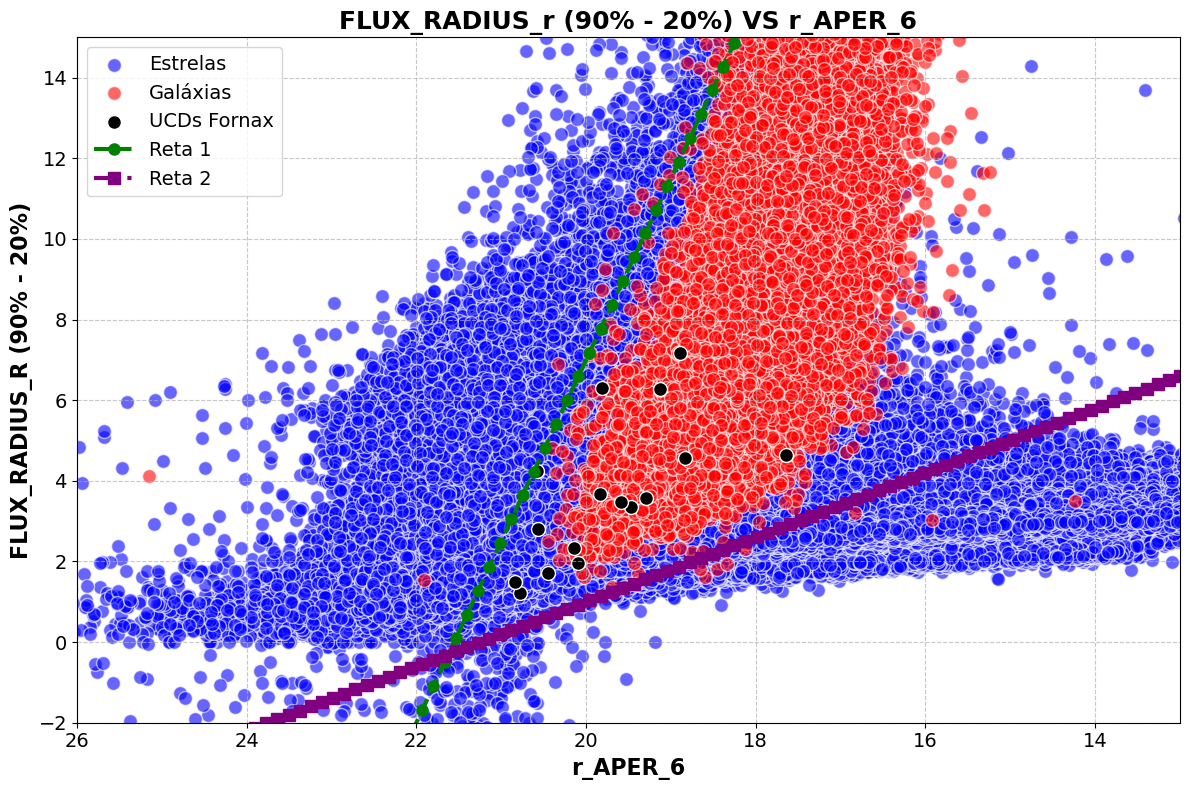
\includegraphics[width=0.8\columnwidth,angle=0]{f_90_20_R_APER_6.png}
    \caption{Gráfico de \text{FLUX\_RADIUS\_90} - \text{FLUX\_RADIUS\_20} em função de \text{r\_APER\_6} para objetos da amostra com classificação estrela-galáxia do GAIA DR3 com probabilidade maior que 90\%. Pontos em azul representam as estrelas, em vermelho as galáxias e em preto as UCDs. As retas em verde e roxo representam os cortes para remover a contaminação de estrelas.}
    \label{flux_radius_1}
    \end{center}
\end{figure}

\begin{figure}[!ht]
    \begin{center}
    % \setcaptionmargin{1cm}
    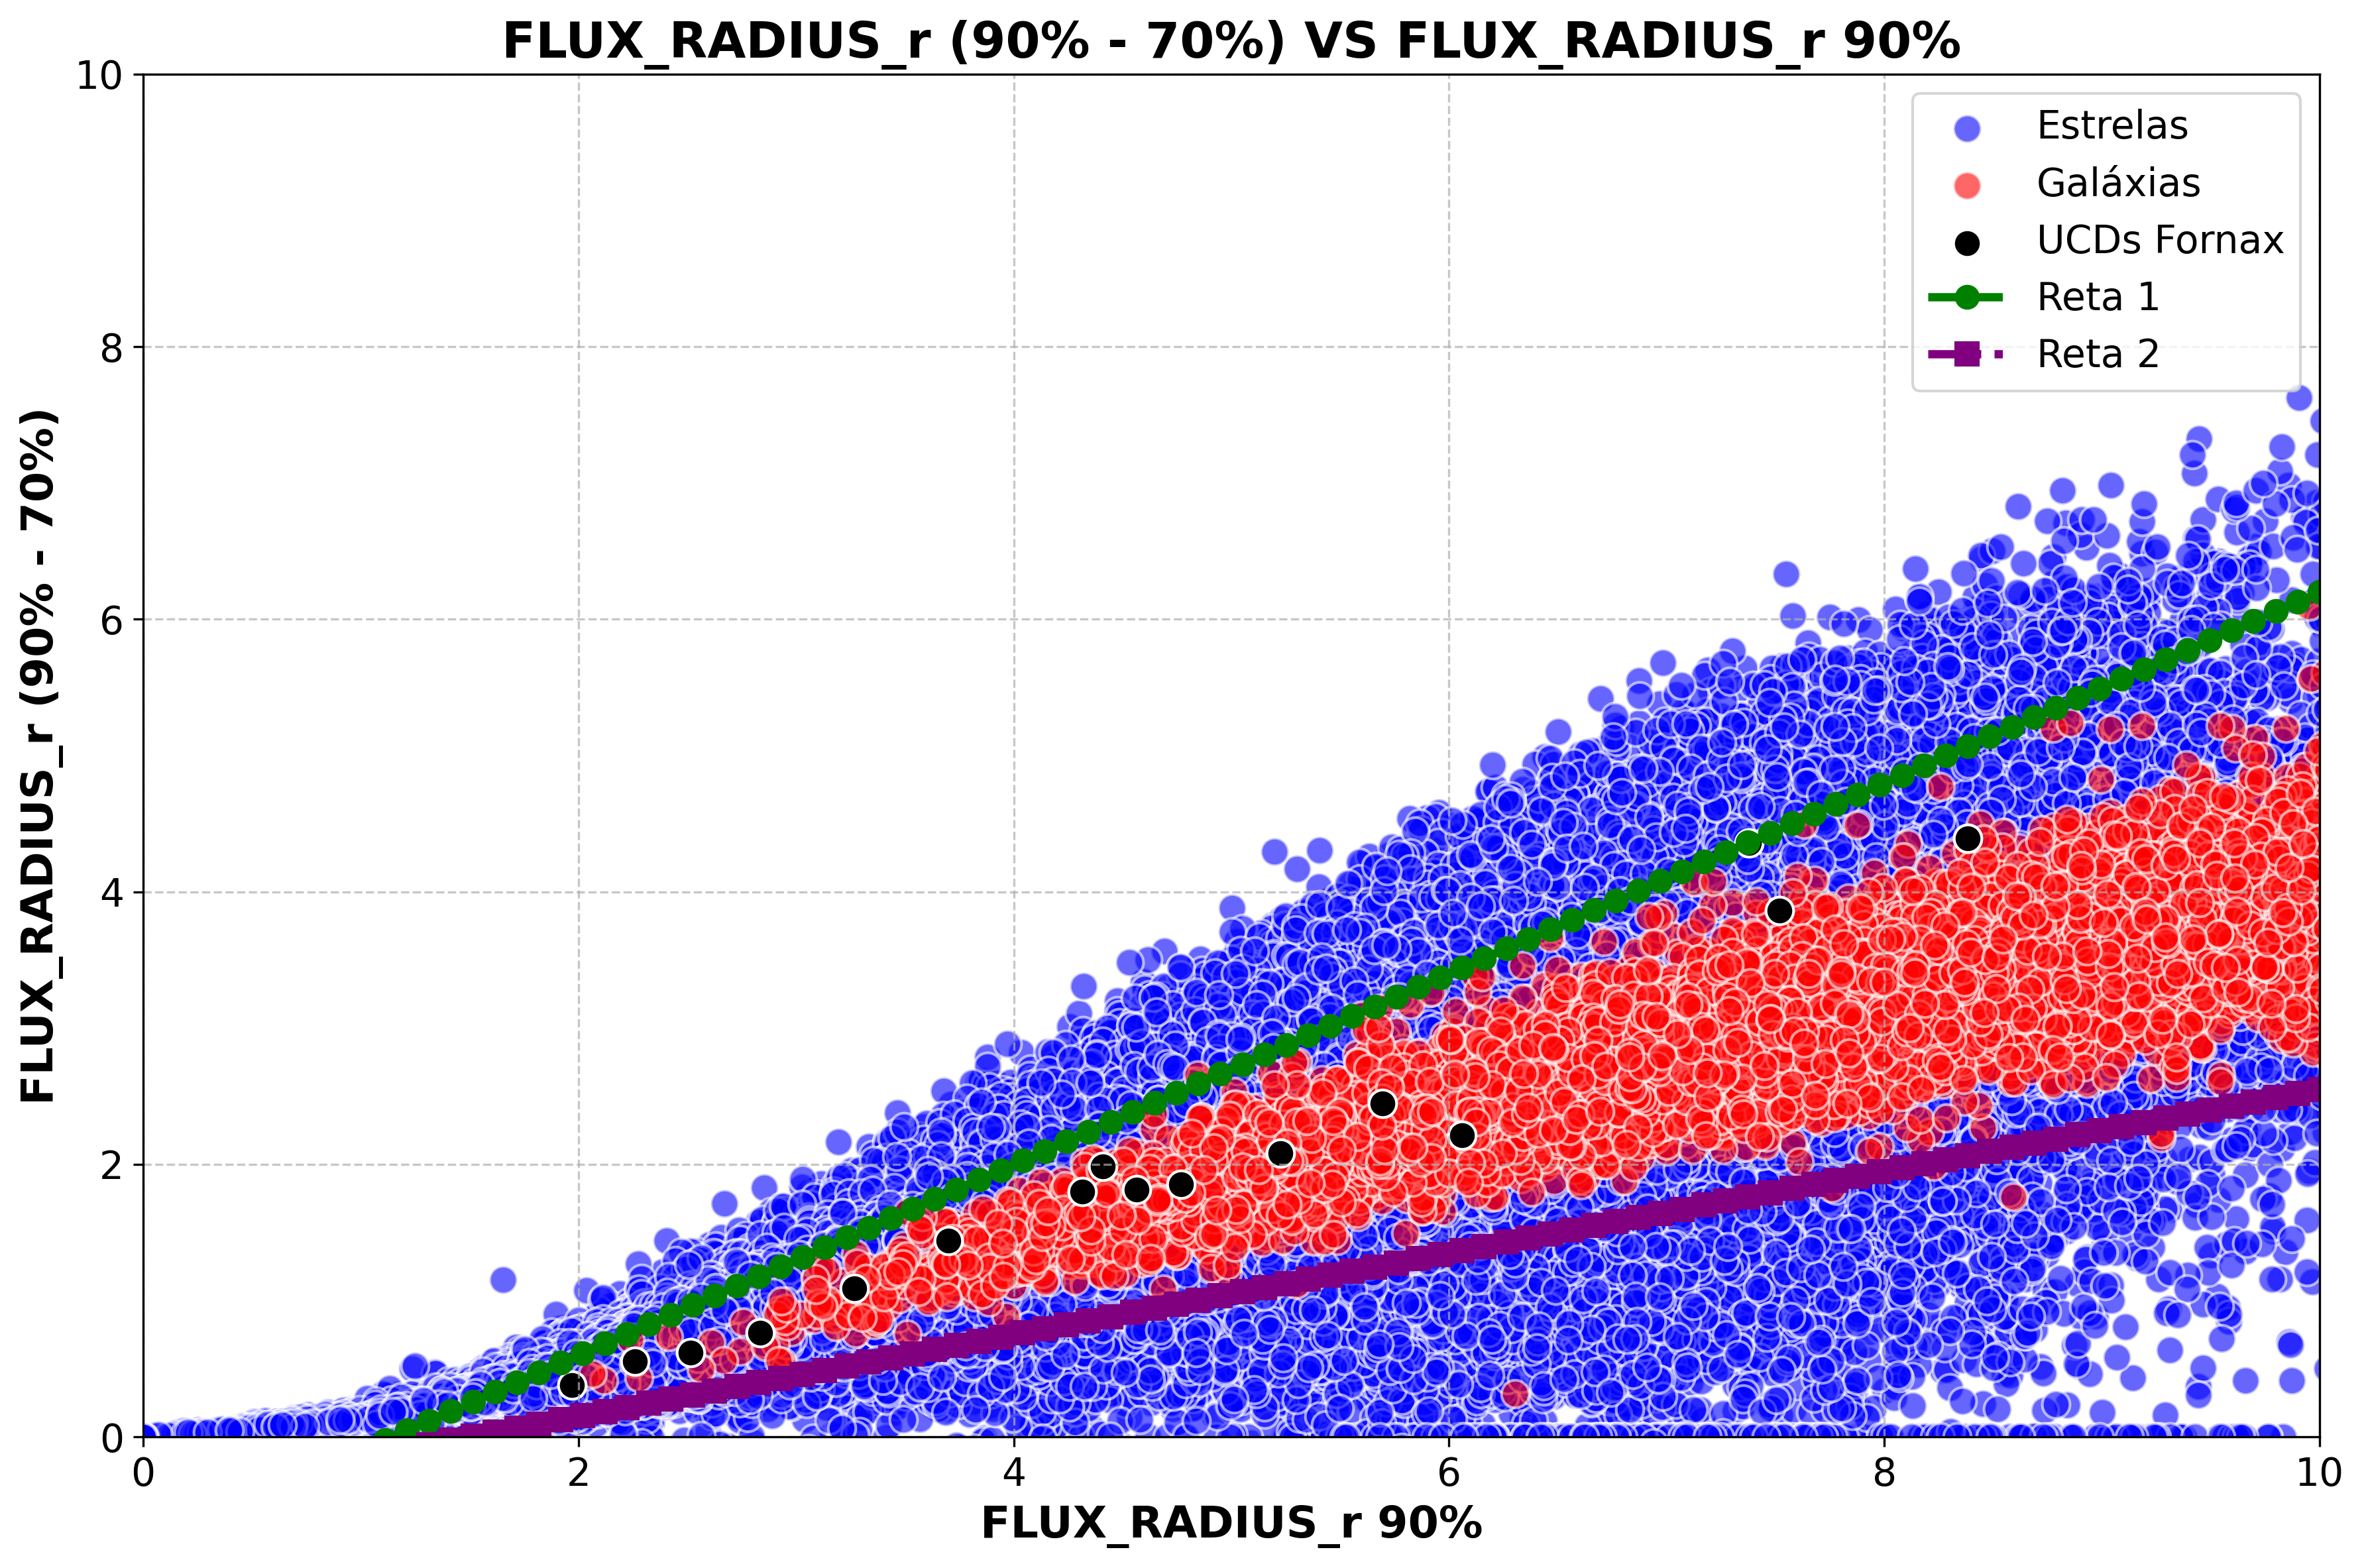
\includegraphics[width=0.8\columnwidth,angle=0]{f_90_70_FLUX_RADIUS_90_R.png}
    \caption[]{Gráfico de \text{FLUX\_RADIUS\_90} - \text{FLUX\_RADIUS\_70} em função de \text{FLUX\_RADIUS\_90} para objetos da amostra com classificação estrela-galáxia do GAIA DR3 com probabilidade maior que 90\%. Pontos em azul representam as estrelas, em vermelho as galáxias e em preto as UCDs. As retas em verde e roxo representam os cortes para remover a contaminação de estrelas.}
    \label{flux_radius_2}
    \end{center}
\end{figure}

\begin{figure}[!ht]
    \begin{center}
    % \setcaptionmargin{1cm}
    \includegraphics[width=0.8\columnwidth,angle=0]{f_70_20_f_90_70.png}
    \caption[]{Gráfico de \text{FLUX\_RADIUS\_70} - \text{FLUX\_RADIUS\_20} em função de \text{FLUX\_RADIUS\_90} - \text{FLUX\_RADIUS\_70} para objetos da amostra com classificação estrela-galáxia do GAIA DR3 com probabilidade maior que 90\%. Pontos em azul representam as estrelas, em vermelho as galáxias e em preto as UCDs. As retas em verde e roxo representam os cortes para remover a contaminação de estrelas.}
    \label{flux_radius_3}
    \end{center}
\end{figure}

Após esses cortes, ficamos com uma amostra de 202.870 objetos. Para seleção de objetos compactos, com base nas classificações do modelo, filtramos aqueles com probabilidade maior que 90\% de serem extensos. A partir dessa amostra, selecionamos as candidatas a UCDs, que são objetos compactos com alta probabilidade de serem extensos, resultando em 9.918 objetos.

Fazendo uso das previsões de redshifts fotométricos da seção \ref{sec:zphot}, iremos remover os objetos com redshifts fotométricos vindos de \citep{erik_photoz_2024}, que são mais robustos que o nosso modelo de redshift. Já para os objetos que não têm redshifts fotométricos disponíveis, iremos usar o mesmo corte, mas para o nosso modelo de regressão de redshifts fotométricos. O corte adotado para o redshift fotométrico é feito para removermos objetos com maiores chances de serem do fundo, e dado os erros do modelo, principalmente para os objetos mais próximos, usaremos um corte mais conservador. Assim, adotamos um corte para os redshifts fotométricos de \textit{$z_{phot}$}$\leq$0.05, que corresponde a um valor de uma ordem de magnitude acima do redshift de Fornax.

Ao final de todo o processo de seleção de candidatas com maiores similaridades com as UCDs, encontramos um total de 242 objetos de uma amostra inicial de aproximadamente 2,9 milhões de objetos no campo de Fornax. O resultado gerado até aqui inclui cortes adotados pelo nosso modelo de classificação, sendo possível replicar o processo para outras amostras de dados. Com essa amostra de candidatas, que representa uma fração menor, porém ainda significativa, podemos partir para uma análise um pouco mais detalhada desses objetos, de maneira a selecionar apenas uma dezena para observação espectroscópica.

Não tínhamos aplicado o corte em uma primeira análise com o GAIA, mas com nossa amostra final, aplicaremos um corte do classificador estelar, para encontrarmos aqueles mais interessantes que mesmo o GAIA classificou como galáxia. Assim, selecionamos aqueles com probabilidade menor que 0.5 de serem estrelas.

Desses objetos, obtivemos uma amostra de 10 candidatos. Observando as imagens dos objetos no Legacy Survey, notamos que parte dos objetos tem uma aparência mais extensa, e mesmo com os valores de \textit{FWHM} menores, apresentam parte de um disco ou braços espirais, e que podem ser objetos de fundo. Assim, escolhemos desses objetos aqueles que têm uma aparência mais pontual, com um critério visual, sem uma segunda componente extensa além do núcleo, selecionando 1 candidata. 

% Selecionamos também mais uma galáxia que, mesmo sendo um pouco mais extensa, está perto de uma galáxia massiva de Fornax, sendo interessante para estudos futuros.

Do restante da amostra de candidatas, com objetos mais fracos, que esperamos que o classificador estelar do GAIA DR3 tenha mais dificuldade em classificar, assim como as UCDs conhecidas mais fracas vistas na Figura \ref{distribuicao_fwhm_image_r_r_aper6_ucds_fornax}, esperamos também encontrar objetos interessantes. Para um critério mais objetivo, fizemos uso do outro classificador galáxia-estrela-quasar do S-PLUS DR4 (\textit{PROB\_GAL}, \textit{PROB\_STAR}, \textit{PROB\_QSO}) \citep{lili_classification}\footnote{Documentação S-PLUS Data Release 5: \url{https://splus.cloud/documentation/idr5}}. Ele oferece uma classificação levando em conta as bandas fotométricas do S-PLUS.

Selecionamos assim os objetos que não foram selecionados pelo corte estelar do GAIA DR3, mas que foram classificados com probabilidade acima de 80\% de ser galáxias pelo S-PLUS DR4. Dessa seleção foram retornados 13 objetos.

Tínhamos 217 objetos na nossa amostra de candidatas, dos quais selecionamos 1 interessante pela classificação de galáxia do GAIA DR3, e mais 13 pela classificação de galáxia do S-PLUS DR4. Assim, temos um total de 14 objetos para a amostra final de candidatas a UCDs em Fornax.

Comparando-os com as UCDs conhecidas, apresentamos na Figura \ref{ucds_and_candiadates_star_cut_photospec} dois gráficos de fotoespectros sobrepostos: o primeiro mostra as UCDs conhecidas, enquanto o segundo exibe os objetos selecionados como candidatas.

\begin{figure}[!ht]
    \centering
    \captionsetup{justification=centering}
    \begin{subfigure}[b]{0.95\textwidth}
        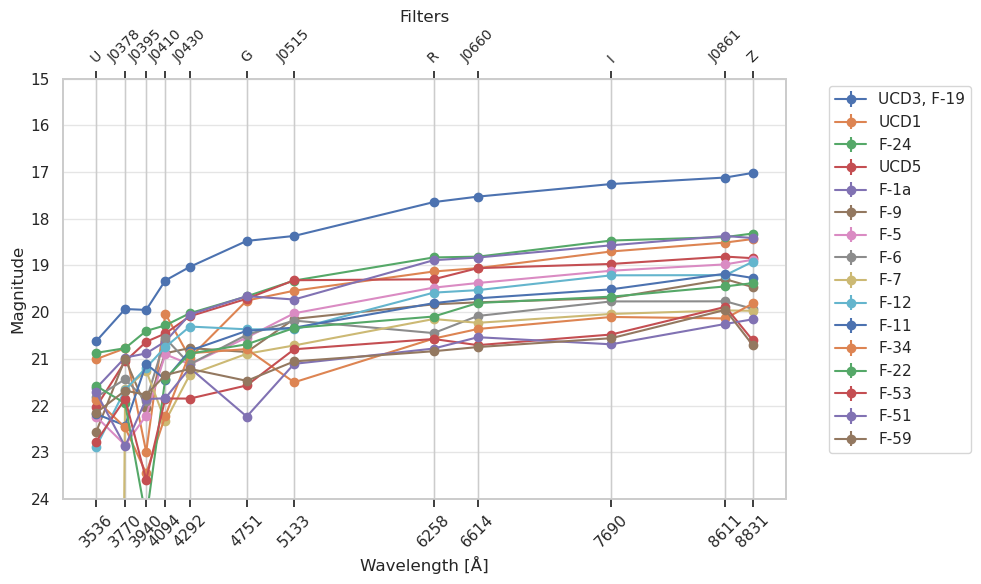
\includegraphics[width=\textwidth]{photo_specs/photospec_ucds.png}
        \caption{Fotoespectros das UCDs conhecidas em Fornax}
    \end{subfigure}
    \begin{subfigure}[b]{0.95\textwidth}
        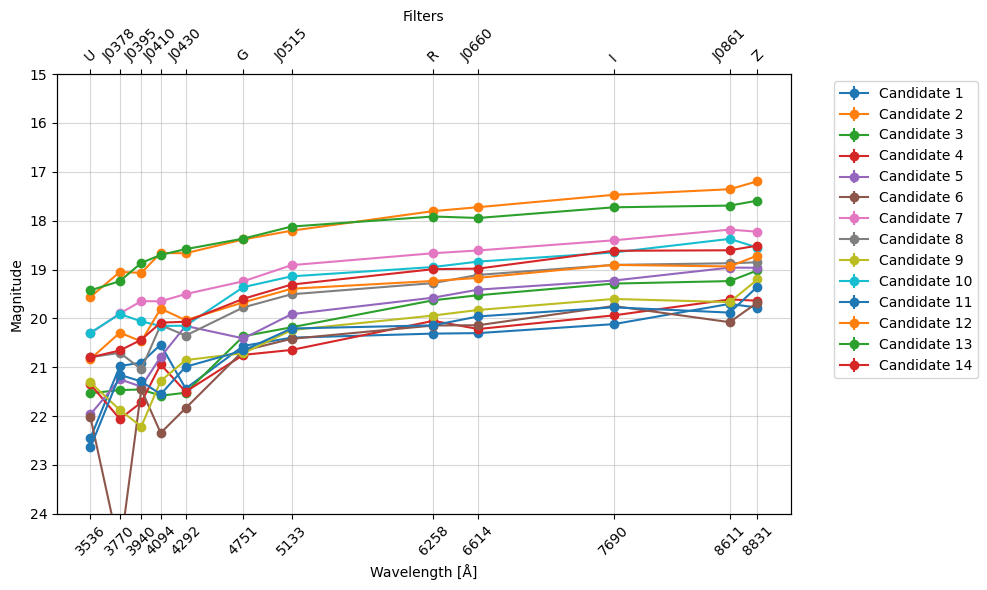
\includegraphics[width=\textwidth]{photo_specs/photospec_candidatas.png}
        \caption{Fotoespectros dos objetos selecionados para candidatas a UCD}
    \end{subfigure}
    \caption{Gráficos de fotoespectros sobrepostos das UCDs conhecidas em Fornax e dos objetos selecionados da amostra de candidatas.}
    \label{ucds_and_candiadates_star_cut_photospec}
\end{figure}


Apresentamos na Figura \ref{ucds_candidates_final_imagens} as imagens dos 14 objetos selecionados como candidatas a UCDs em Fornax.

\begin{figure}[!ht]
    \centering
    \captionsetup{justification=centering}
    \begin{subfigure}[b]{0.25\textwidth}
        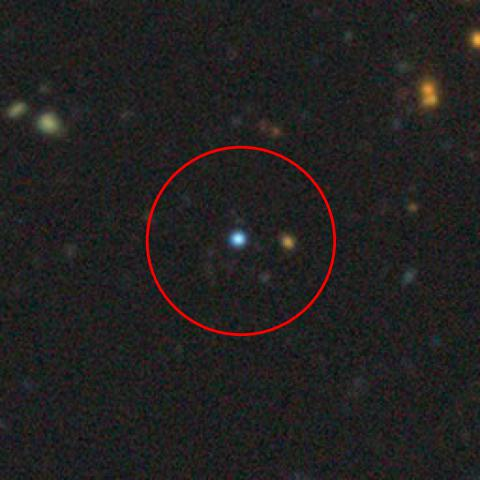
\includegraphics[width=\textwidth]{candidata_final/01.jpg}
        \caption{Candidata 01}
    \end{subfigure}
    \begin{subfigure}[b]{0.25\textwidth}
        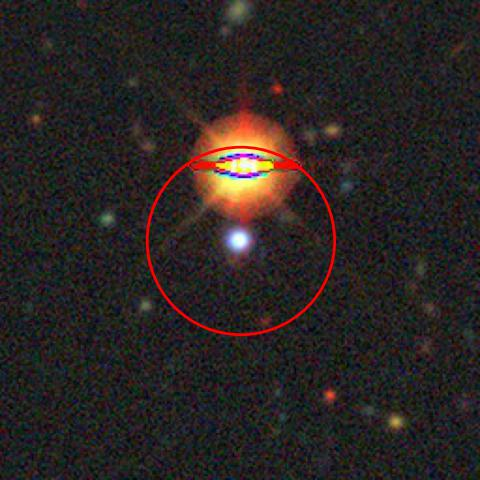
\includegraphics[width=\textwidth]{candidata_final/02.jpg}
        \caption{Candidata 02}
    \end{subfigure}
    \begin{subfigure}[b]{0.25\textwidth}
        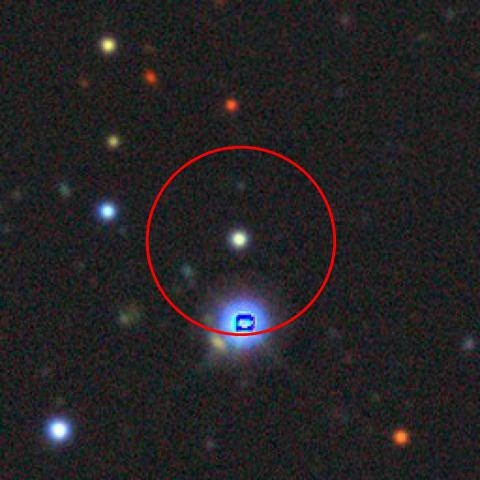
\includegraphics[width=\textwidth]{candidata_final/03.jpg}
        \caption{Candidata 03}
    \end{subfigure}
    \begin{subfigure}[b]{0.25\textwidth}
        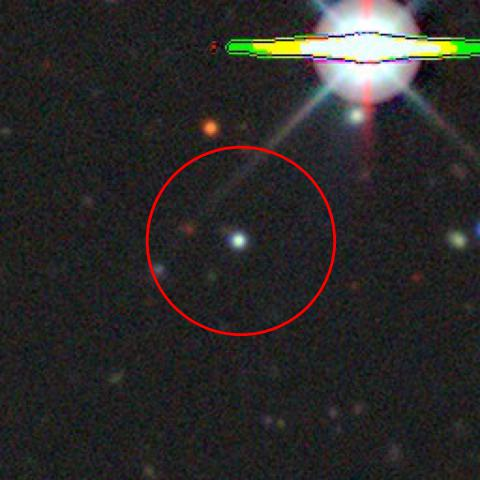
\includegraphics[width=\textwidth]{candidata_final/04.jpg}
        \caption{Candidata 04}
    \end{subfigure}
    \begin{subfigure}[b]{0.25\textwidth}
        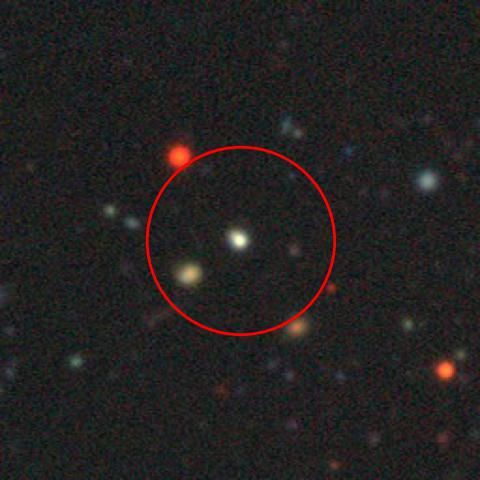
\includegraphics[width=\textwidth]{candidata_final/05.jpg}
        \caption{Candidata 05}
    \end{subfigure}
    \begin{subfigure}[b]{0.25\textwidth}
        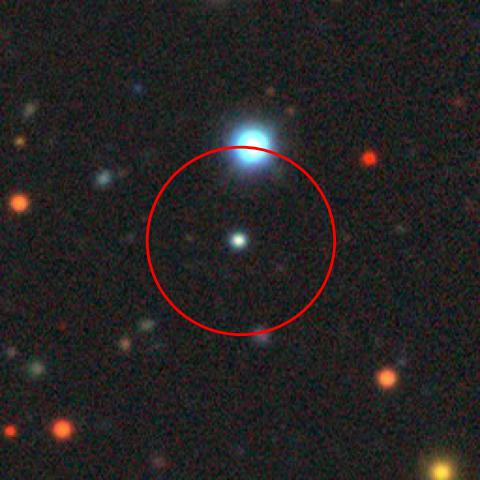
\includegraphics[width=\textwidth]{candidata_final/06.jpg}
        \caption{Candidata 06}
    \end{subfigure}
    \begin{subfigure}[b]{0.25\textwidth}
        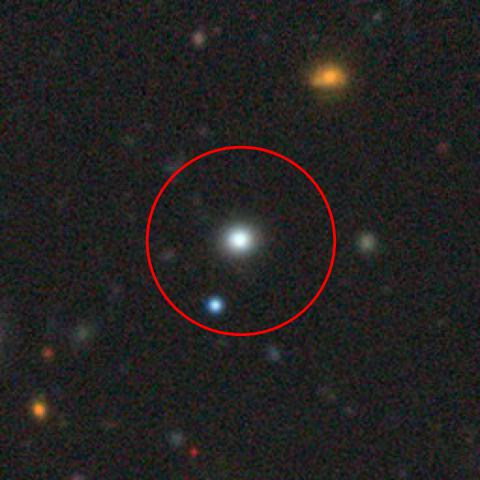
\includegraphics[width=\textwidth]{candidata_final/07.jpg}
        \caption{Candidata 07}
    \end{subfigure}
    \begin{subfigure}[b]{0.25\textwidth}
        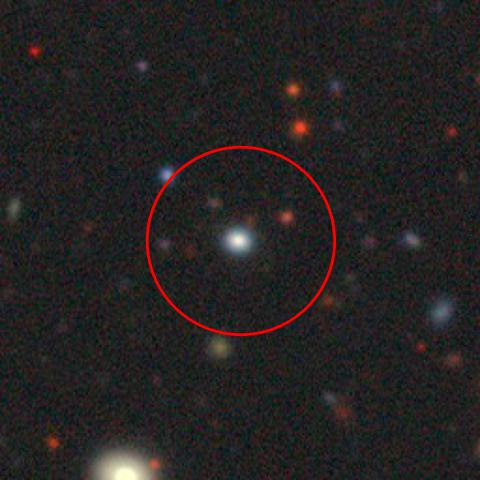
\includegraphics[width=\textwidth]{candidata_final/08.jpg}
        \caption{Candidata 08}
    \end{subfigure}
    \begin{subfigure}[b]{0.25\textwidth}
        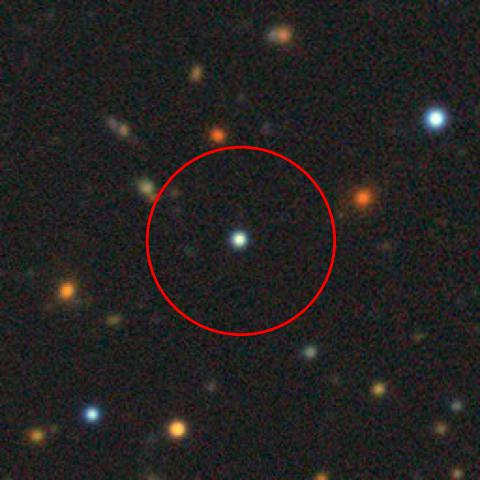
\includegraphics[width=\textwidth]{candidata_final/09.jpg}
        \caption{Candidata 09}
    \end{subfigure}
    \begin{subfigure}[b]{0.25\textwidth}
        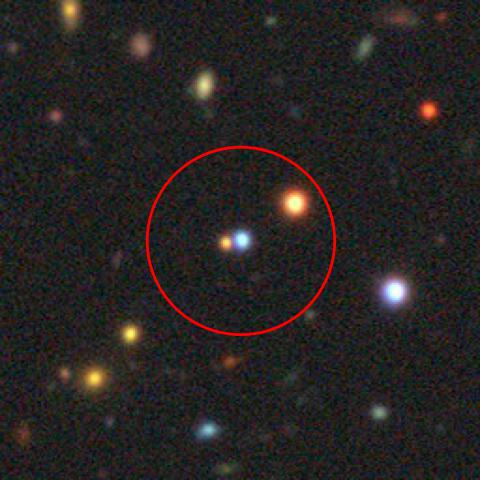
\includegraphics[width=\textwidth]{candidata_final/10.jpg}
        \caption{Candidata 10}
    \end{subfigure}
    \begin{subfigure}[b]{0.25\textwidth}
        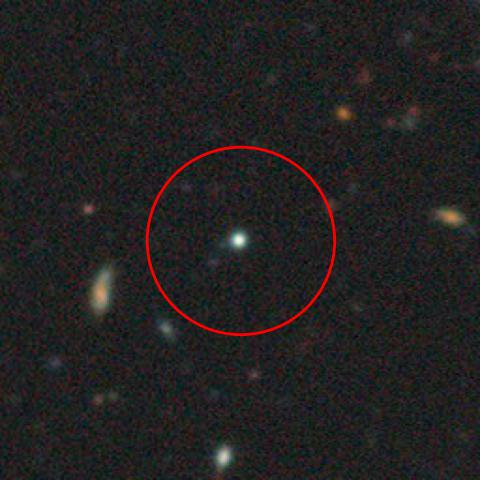
\includegraphics[width=\textwidth]{candidata_final/11.jpg}
        \caption{Candidata 11}
    \end{subfigure}
    \begin{subfigure}[b]{0.25\textwidth}
        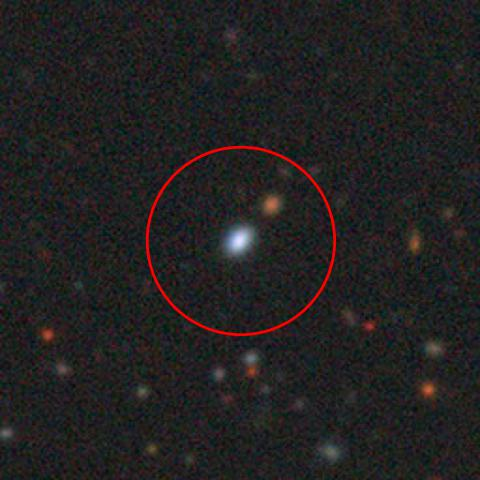
\includegraphics[width=\textwidth]{candidata_final/12.jpg}
        \caption{Candidata 12}
    \end{subfigure}
    \begin{subfigure}[b]{0.25\textwidth}
        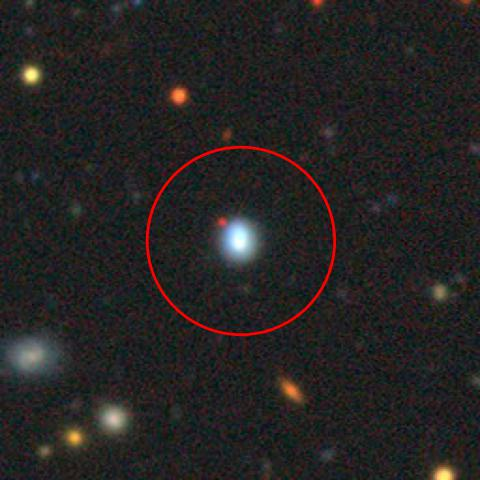
\includegraphics[width=\textwidth]{candidata_final/13.jpg}
        \caption{Candidata 13}
    \end{subfigure}
    \begin{subfigure}[b]{0.25\textwidth}
        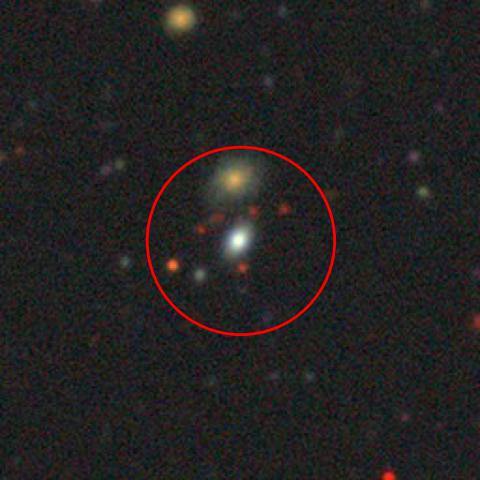
\includegraphics[width=\textwidth]{candidata_final/14.jpg}
        \caption{Candidata 14}
    \end{subfigure}
    \caption[]{Imagens das candidatas finais a UCDs. Imagens obtidas pelo Legacy Survey.}
    \label{ucds_candidates_final_imagens}
\end{figure}



\section{Análise das candidatas}\label{sec:analise_candidatas}
Selecionamos 14 objetos para a amostra final de candidatas a UCDs da seção \ref{sec:selecao_candidatas}.
%  mais 4 objetos com possíveis sinais de emissão da subseção \ref{subsec: candidatas_emissao}, totalizando 21 objetos.

Utilizando o catálogo de Fornax proveniente do projeto S-PLUS Fornax \citep{castelli2024splusfornaxprojectsfp}, com a fotometria apresentada por \citep{haack2024splusfornaxprojectsfp}, obtivemos uma amostra de galáxias conhecidas, classificadas morfologicamente. Com base nisso, realizamos uma análise das candidatas selecionadas, comparando-as com as galáxias conhecidas. Identificamos, em diversos conjuntos de parâmetros, tanto a localização das UCDs reais quanto a posição das nossas candidatas.

Selecionamos as categorias morfológicas de galáxias mais relevantes com as maiores quantidades de objetos para comparação. Dentre elas, temos as galáxias anãs elípticas, nucleadas e não nucleadas, junto das irregulares. Outros tipos importantes incluem as LSB (Low Surface Brightness) e as galáxias espirais.

Analisamos como as UCDs e as galáxias conhecidas, classificadas morfologicamente, se distribuem em diferentes espaços de parâmetros, especialmente aqueles que representam a morfologia de objetos compactos. Um dos parâmetros avaliados foi o brilho superficial médio, aqui calculado na banda $r$, que mede a densidade superficial de luminosidade média de um objeto. Ele foi obtido a partir da magnitude aparente e do raio efetivo do objeto.

Utilizamos o parâmetro \textit{PETRO\_RADIUS}, fornecido pelo SExtractor, que está em unidades dos semieixos \textit{A} ou \textit{B}, para calcular o raio do objeto em cada um dos dois semieixos. A partir disso, determinamos o brilho superficial médio, somando a magnitude aparente a 2,5 vezes o logaritmo da área da elipse, convertida para unidades de arcsec$^2$ (multiplicando pelo fator de 0,55 arcsec/pixel para cada semieixo). A equação utilizada para o cálculo do brilho superficial médio é:

\begin{equation}
    \mu_{\text{medio}} = \text{mag\_aparente} + 2.5 \times \log_{10}(\pi \times A \times B \times 0.55^2 \times \text{PETRO\_RADIUS}^2)
    \label{equation_sb}
\end{equation}

Na Figura \ref{sb_r_ucds_galaxias}, mostramos a distribuição do brilho superficial médio na banda $r$ para as UCDs conhecidas e as galáxias morfologicamente classificadas, juntamente com as candidatas selecionadas.

\begin{figure}[!ht]
    \begin{center}
    \includegraphics[width=1.\columnwidth,angle=0]{sb_r_ucds_galaxias.png}
    \caption[]{Magnitude superficial média na banda $r$ em função da magnitude aparente na banda $r$ para as UCDs conhecidas, as galáxias morfologicamente classificadas e as candidatas selecionadas.}
    \label{sb_r_ucds_galaxias}
    \end{center}
\end{figure}

A Figura \ref{sb_r_ucds_galaxias} mostra que, para parte das galáxias com morfologia conhecida apresentadas, elas seguem uma distribuição em cauda para o brilho superficial médio na banda $r$, em função da magnitude aparente na banda $r$. Já as UCDs conhecidas e as candidatas estão localizadas na parte inferior. Esse fato indica que, para um mesmo brilho superficial médio, as UCDs e as candidatas são menos brilhantes que as galáxias de morfologia apresentada, que são mais extensas. Além disso, para uma mesma magnitude aparente, as UCDs e as candidatas apresentam um brilho superficial médio menor (mais brilhante) do que as galáxias do tipo dE, por exemplo. Isso ocorre porque elas são mais compactas, com raios efetivos menores, resultando em uma maior concentração de luz em uma área reduzida.

Tanto para os cenários previstos de formação das UCDs como núcleos expostos de galáxias anãs que foram despojadas de suas camadas externas por interações gravitacionais em aglomerados, quanto para aqueles de formação a partir de aglomerados estelares massivos, o resultado são objetos com alta densidade estelar e raios efetivos pequenos.

Nesse tipo de diagrama, quando comparado com as galáxias de morfologia “convencional” (elípticas, espirais, etc.), essa diferença estrutural dos dois tipos é evidenciada: as UCDs ocupam uma região “compacta e luminosa” para seu tamanho, enquanto as galáxias seguem uma correlação mais “espalhada” entre luminosidade e tamanho/brilho superficial.

Na Figura \ref{r_aper_6_mu_max} e \ref{r_aper_6_kron_radius}, temos os parâmetros \textit{MU\_MAX} e \textit{KRON\_RADIUS}, respectivamente, ambos em função da magnitude aparente na banda $r$. O \textit{MU\_MAX} representa o pico de brilho superficial do objeto, indicando o quão brilhante é a região central do objeto em comparação com o fundo. Já o \textit{KRON\_RADIUS} (raio de Kron) é um raio adaptativo calculado pelo SExtractor a partir da média ponderada da distância dos pixels ao centro do objeto, com base na distribuição de luz.

Em ambas as figuras, observamos que as candidatas se localizam em regiões mais próximas das UCDs conhecidas do que das demais galáxias com morfologia apresentada. Na Figura \ref{r_aper_6_mu_max}, vemos que elas seguem uma segunda curva abaixo das galáxias mais extensas. Já para a Figura \ref{r_aper_6_kron_radius}, vemos que, conforme os objetos ficam mais fracos, o raio de Kron aumenta. Quando um objeto é mais extenso ou tem a luz distribuída de forma difusa, a ferramenta precisa usar um raio maior para abranger boa parte do fluxo total. Em outras palavras, objetos mais fracos (mas espalhados em área maior) resultam em um Kron Radius maior, pois o algoritmo “enxerga” a luz se estendendo além de um núcleo compacto. Já objetos brilhantes e concentrados apresentam Kron Radius menor, pois a maior parte do fluxo está contida numa região pequena. Ainda assim, notamos que as candidatas selecionadas e UCDs conhecidas têm a mesma tendência, porém agrupadas em uma região mais abaixo do gráfico.

\begin{figure}[!ht]
    \begin{center}
    \includegraphics[width=1.\columnwidth,angle=0]{r_aper_6_mu_max.png}
    \caption[]{Parâmetro \textit{MU\_MAX} em função da magnitude aparente na banda $r$ para as UCDs conhecidas, as galáxias morfologicamente classificadas e as candidatas selecionadas.}
    \label{r_aper_6_mu_max}
    \end{center}
\end{figure}


\begin{figure}[!ht]
    \begin{center}
    \includegraphics[width=1.\columnwidth,angle=0]{r_aper_6_kron_radius.png}
    \caption[]{Parâmetro \textit{KRON\_RADIUS} em função da magnitude aparente na banda $r$ para as UCDs conhecidas, as galáxias morfologicamente classificadas e as candidatas selecionadas.}
    \label{r_aper_6_kron_radius}
    \end{center}
\end{figure}

Pela análise dos gráficos, concluímos que as candidatas selecionadas estão localizadas nas mesmas regiões que as UCDs conhecidas. Isso é um forte indicativo de que as candidatas possuem características semelhantes às UCDs conhecidas.

Mostramos na Figura \ref{distribuicao_candidatas_radec} a distribuição em coordenadas equatoriais das candidatas selecionadas, juntamente com as UCDs conhecidas e o compilado das galáxias massivas.

\begin{figure}[!ht]
    \begin{center}
    \includegraphics[width=1.\columnwidth,angle=0]{distribuicao_candidatas_radec.png}
    \caption[]{Distribuição em coordenadas equatoriais (RA, DEC) das candidatas a UCDs selecionadas (estrelas azuis), comparadas com as UCDs conhecidas (círculos verdes) e as galáxias massivas (triângulos roxos) no aglomerado de Fornax. O fundo vermelho representa a área de cobertura dos dados do S-PLUS. Os círculos tracejados em roxo indicam um raio de 200 kpc ao redor de cada galáxia massiva. O arco preto corresponde ao raio de virial do aglomerado (700 kpc).}
    \label{distribuicao_candidatas_radec}
    \end{center}
\end{figure}

A Figura \ref{distribuicao_candidatas_radec} apresenta o principal resultado da nossa seleção e busca por candidatas a UCDs no aglomerado de Fornax. Observando as imagens das candidatas na Figura \ref{ucds_candidates_final_imagens}, notamos que elas possuem uma aparência mais pontual, como esperado para objetos compactos. Essas candidatas representam uma seleção de objetos que exibem características morfológicas e fotométricas consistentes com as UCDs conhecidas.

Elas foram selecionadas com base em múltiplos critérios: possuem larguras à meia altura (\textit{FWHM}) compatíveis com objetos compactos, altas probabilidades de serem extensos segundo o modelo de aprendizado de máquina, redshifts fotométricos que indicam baixa probabilidade de serem objetos de fundo muito distantes do aglomerado, e magnitudes dentro do intervalo esperado para UCDs. Além disso, as análises das distribuições de parâmetros, como o brilho superficial médio (Figura \ref{sb_r_ucds_galaxias}), o pico de brilho superficial (\textit{MU\_MAX}, Figura \ref{r_aper_6_mu_max}) e o raio de Kron (\textit{KRON\_RADIUS}, Figura \ref{r_aper_6_kron_radius}), mostram que essas candidatas ocupam as mesmas regiões que as UCDs conhecidas, reforçando sua similaridade estrutural e fotométrica.

Esses resultados indicam que as candidatas selecionadas são os objetos mais promissores para estudos espectroscópicos futuros, com uma combinação de critérios morfológicos, fotométricos e probabilísticos aplicada neste trabalho.

Na Figura \ref{distribuicao_candidatas_radec}, observamos que, das 14 candidatas, apenas uma está localizada dentro do raio de virial do aglomerado, enquanto as demais estão distribuídas em regiões mais externas, especialmente nas coordenadas mais à direita da imagem.

As UCDs conhecidas até o momento são predominantemente encontradas em regiões centrais de aglomerados de galáxias. Essa concentração nas áreas mais densas pode ser explicada pelo viés observacional, uma vez que estudos espectroscópicos intensivos geralmente se concentram nas regiões centrais dos aglomerados, onde a densidade de galáxias é maior. Esse viés justifica a ausência de UCDs conhecidas em regiões mais externas do aglomerado de Fornax.

A amostra de candidatas selecionadas neste trabalho apresenta características consistentes com UCDs conhecidas, indicando potencial para serem confirmadas como novas UCDs, especialmente em regiões periféricas do aglomerado de Fornax. A presença dessas candidatas em áreas externas sugere que UCDs podem se formar em ambientes menos densos e, posteriormente, migrar para regiões centrais devido a processos dinâmicos.

Modelos baseados em interações gravitacionais intensas, como o stripping de galáxias anãs nucleadas, requerem tipicamente ambientes densos, como os centros dos aglomerados, onde essas interações são mais frequentes \citep{Bekki_2001,Pfeffer_2016}. Nesse contexto, a formação de UCDs seria diretamente dependente do ambiente de aglomerado, e sua concentração central observada em outros trabalhos reforça esse cenário. 

Entretanto, a distribuição periférica das candidatas identificadas neste trabalho também é compatível com cenários de formação que não exigem necessariamente a presença de um ambiente denso como o núcleo de um aglomerado. Entre esses mecanismos alternativos estão a fusão de superaglomerados estelares formados \textit{in situ} em regiões de menor densidade \citep{Mieske_2011}, bem como o colapso direto de nuvens de gás primordial, que pode originar núcleos compactos e massivos \citep{Drinkwater_2003}. Esses processos são particularmente plausíveis em subestruturas em \textit{infall} ou em halos galácticos pouco perturbados, o que se alinha com a localização observada das candidatas.

Embora \citet{Bekki_2001} tenham mostrado que o stripping de galáxias anãs nucleadas tende a produzir UCDs concentradas nos centros de aglomerados, modelos mais recentes (e.g., \citealt{Br_ns_2011}; \citealt{Mieske_2011}; \citealt{Pfeffer_2016}) preveem populações mais distribuídas espacialmente, incluindo objetos em regiões periféricas. Assim, nossos resultados fortalecem a hipótese de que múltiplos canais de formação, refletindo a diversidade morfológica, dinâmica e espacial das UCDs. Caso a presença de UCDs se estenda de fato para regiões além do raio de virial, isso reforça a necessidade de incluir modos de crescimento contínuo e eventos de \textit{infall} tardio nos modelos semianalíticos de formação de galáxias (SAMs), conforme sugerido por \citet{Pfeffer_2016}.

Assim, a descoberta de candidatas a UCDs fora do raio de virial de Fornax não só ampliaria significativamente a população conhecida, mas também nos obrigaria a repensar os processos de formação e evolução dessas galáxias compactas, explorando ativamente ambientes de baixa densidade e ampliando nosso entendimento sobre a distribuição espacial e os mecanismos de formação das UCDs.



\chapter{\chapternamespectra}\label{chap:spectra}
A fotometria é uma ferramenta poderosa para o estudo em grande escala de objetos astronômicos, pois permite detectar muitos alvos simultaneamente em um campo de visão amplo. Em particular, fotometrias multibanda, como a do S-PLUS, fornecem dados de objetos com diferentes características espectrais. No entanto, embora os dados fotométricos sejam extremamente úteis para a seleção de objetos, eles não são suficientes para confirmar a natureza dos alvos observados. Para isso, é necessário realizar observações espectroscópicas, que permitem identificar características como linhas de emissão e absorção presentes nos espectros dos objetos, confirmando sua natureza e redshift.

A espectroscopia é uma técnica essencial para a análise detalhada da luz emitida ou absorvida por um objeto, revelando informações sobre sua composição química, temperatura, densidade e movimento. Neste trabalho, a espectroscopia desempenha um papel crucial na confirmação da natureza dos objetos selecionados. Em particular, estamos interessados em determinar o redshift dos objetos, o que nos permite calcular suas distâncias e verificar se eles pertencem ao aglomerado de Fornax. Além disso, a espectroscopia nos ajuda a identificar se a natureza compacta dos objetos selecionados é real ou apenas um efeito de projeção.

Neste capítulo, apresentamos os dados espectroscópicos obtidos com o telescópio Gemini Sul, utilizados para analisar as candidatas a galáxias ultracompactas (UCDs) no aglomerado de Fornax. A seção \ref{sec:gemini} descreve o telescópio Gemini Sul e os dados obtidos. Na seção \ref{sec:manipulando_espectros}, discutimos o processo de redução dos espectros, incluindo a limpeza dos dados e a análise das linhas de emissão e absorção. A seção \ref{sec:analise_espectros} apresenta os resultados da análise dos espectros das candidatas observadas, enquanto a seção \ref{sec:objetos_linhas_emissao} discute os objetos com linhas de emissão identificados durante a análise.

\section{Dados telescópio Gemini Sul}\label{sec:gemini}
O Observatório Gemini é uma instalação astronômica internacional composta por dois telescópios gêmeos: um localizado no hemisfério norte, no Havaí, e outro no hemisfério sul, no Chile. O Gemini South, situado no Chile, é equipado com um espelho primário de 8,1 metros de diâmetro (assim como o Gemini North).

Para buscar novas galáxias ultracompactas no aglomerado de Fornax, a partir das candidatas identificadas pela metodologia adotada neste trabalho, é necessário realizar confirmações espectroscópicas. Essas confirmações são importantes para verificar se as candidatas são de fato galáxias e se elas estão no redshift do aglomerado de Fornax. Para isso, utilizamos dados espectroscópicos obtidos do GMOS-S, instalado no telescópio Gemini South.

Como parte deste projeto, algumas candidatas preliminares já haviam sido selecionadas em um trabalho de iniciação científica anterior. Nesse contexto, analisamos os dados espectroscópicos dessas candidatas prévias, além de solicitar e analisar novos dados espectroscópicos obtidos para as novas candidatas identificadas neste estudo.

Os dados espectroscópicos foram obtidos através do repositório online do Gemini Observatory\footnote{Gemini Observatory, \textit{Gemini Observatory Archive}, disponível em \url{https://archive.gemini.edu}}.

% \begin{itemize}
%     \item \textbf{Telescópio}: GMOS-S no Gemini South.
%     \item \textbf{Modo de Observação}: Modo de fenda longa.
%     \item \textbf{Gratinete}: B600-G5303 com comprimento de onda central $\lambda_c = 550 \, \text{nm}$ e fenda de 1,500 $\mu\text{m}$.
%     \item \textbf{Intervalo Espectral}: [4000\,\text{Å} - 7000\,\text{Å}]
%     \item \textbf{Resolução}: $R \approx 570$.
%     \item \textbf{Tempo de Exposição}: 1200 segundos por alvo
%     \item \textbf{S/N Desejada}: Mínimo de 5 no continuum (S/N $\sim$ 3 por pixel espectral) e S/N $\sim$ 20 nas linhas de emissão.
% \end{itemize}

Para observar as candidatas a galáxias ultracompactas (UCDs) no aglomerado de Fornax, utilizamos o espectrógrafo GMOS-S no telescópio Gemini Sul, operando no modo de fenda longa. Essa abordagem permitiu obter espectros individuais de cada objeto, possibilitando a observação de linhas de emissão e absorção para determinar propriedades globais e confirmar a associação ao aglomerado.

As configurações utilizadas para as observações foram as seguintes:

\begin{itemize}
    \item \textbf{Modo de Observação}: Fenda longa (\textit{long-slit}).
    \item \textbf{Grating}: B600-G5303, com comprimento de onda central $\lambda_c = 550 \, \text{nm}$.
    \item \textbf{Largura da Fenda}: 1,5".
    \item \textbf{Resolução Espectral}: $R \sim 570$, considerando a largura da fenda escolhida.
    \item \textbf{Intervalo Espectral}: 4000\,\text{Å} a 7000\,\text{Å}, cobrindo desde o ultravioleta até o óptico no referencial de repouso.
    \item \textbf{Tempo de Exposição por Objeto}: 1200 segundos, divididos em 3 exposições de 400 segundos cada.
    \item \textbf{Condições de Observação}: IQ=ANY, CC=80\%, WV=ANY, SB=80\%.
    \item \textbf{Razão Sinal-Ruído (S/N) Desejada}: Mínimo de 5 no espectro combinado (equivalente a S/N $\sim$ 3 por pixel espectral) no contínuo, suficiente para detectar o declive do contínuo azul e as principais linhas de absorção.
\end{itemize}

Além disso, foi necessário considerar os tempos de preparação do telescópio, ajustes de guiagem e observações das lâmpadas de calibração de comprimento de onda utilizando linhas de emissão de CuAr. Esses tempos adicionais resultaram em um overhead total de aproximadamente 22 minutos por objeto, incluindo o tempo de leitura e gravação no sistema de manuseio de dados (\textit{Data Handling System, DHS}).

\section{Manipulando os espectros}\label{sec:manipulando_espectros}
Nessa seção, discutiremos o processo de redução dos dados espectroscópicos obtidos do telescópio Gemini Sul. A redução dos dados espectroscópicos é uma etapa crucial para garantir a qualidade e a precisão das análises subsequentes. Essa etapa envolve a correção de artefatos instrumentais, a calibração de fluxos e a extração de espectros unidimensionais (1D) a partir de imagens bidimensionais (2D).

\subsection{Redução dos espectros}\label{subsection:reduzindo_espectros}
Os dados espectroscópicos do telescópio Gemini não passam por um tratamento inicial, então é necessário um pré-processamento. Esse passo é crucial para limpar as imagens de sinais indesejados, removendo ruídos dos instrumentos e convertendo os espectros bidimensionais em unidimensionais para análise.

Fizemos a redução dos dados usando o Software de Redução de Dados DRAGONS (Data Reduction for Astronomy with Gemini Observatory's Node System) \cite{dragons_python}. Esse software permite reduzir os dados tanto pela linha de comando quanto por meio de uma API em Python. Optamos pela API em Python para tornar o processo mais eficiente e agilizar a geração dos espectros unidimensionais (1D) e bidimensionais (2D) para cada objeto.

\textbf{Seleção de Dados}

O primeiro passo para a redução é a seleção dos dados que serão usados, como os arquivos de \textit{bias}, \textit{flats}, \textit{arcs}, estrelas padrão (\textit{standard star}) e os dados científicos. Utilizamos a função \verb|dataselect.select_data|, que permite filtrar os arquivos por algumas características específicas, como o tipo de detector e o objeto observado.

\textbf{Redução do \textit{Bias}}

A etapa inicial da redução é a correção de \textit{bias}, onde os arquivos são processados para remover o sinal eletrônico residual presente nas imagens. Utilizando a função \verb|Reduce|, criamos dois conjuntos de arquivos de \textit{bias}: um para as estrelas padrão e outro para os dados científicos. Essa correção visa garantir que o sinal obtido nas observações não seja contaminado por ruídos instrumentais.

\textbf{Redução dos \textit{Flats}}

Após a correção de \textit{bias}, processamos as imagens de \textit{flat-field}, que corrigem variações na resposta do detector em diferentes regiões do campo de visão. Os arquivos de \textit{flats} são selecionados e processados novamente com a função \verb|Reduce|, assegurando a uniformidade na resposta do detector em todas as partes do espectro.

\textbf{Redução dos \textit{Arcs}}

Na sequência, realizamos a redução dos arquivos de \textit{arcs}, que contêm linhas de emissão conhecidas utilizadas para calibrar a escala de comprimento de onda dos espectros. A função \verb|Reduce| é aplicada para processar os \textit{arcs}, ajustando as linhas de emissão observadas ao modelo teórico e garantindo que os comprimentos de onda sejam medidos com precisão.

\textbf{Redução da Estrela Padrão}

Para a redução da estrela padrão (\textit{standard star}), também utilizamos a função \verb|Reduce| para processar essas observações, gerando um espectro calibrado em fluxo, que serve como referência para a normalização dos espectros dos objetos científicos. O espectro resultante é plotado e analisado para verificar a qualidade da calibração.

\textbf{Redução dos Dados Científicos}

Finalmente, os dados científicos são reduzidos aplicando todas as correções anteriores (\textit{bias}, \textit{flat}, \textit{arc}) aos dados de observação dos objetos de interesse, novamente utilizando a função \verb|Reduce|. Esse processo resulta na geração dos espectros unidimensionais (\textit{1D}) e bidimensionais (\textit{2D}) que poderão ser analisados.

\subsection{Análise dos espectros}\label{subsection:analisespectros}
Após os pedidos de tempo de observação no Gemini Sul, obtivemos os espectros das candidatas selecionadas. A partir desses dados, realizamos a análise dos espectros para identificar as características dos objetos observados. Usamos o programa PYRAF, uma linguagem de comando para IRAF baseada na linguagem de script Python, que pode ser usada para análise espectral dos objetos de interesse.

Com os espectros brutos reduzidos pelo DRAGONS, antes de qualquer análise, precisamos limpar os dados de ruídos e remover sinais indesejados. Primeiro, removemos possíveis linhas de céu e raios cósmicos, que afetam nossos espectros. Na Figura \ref{exemplo_remocao_linhas_ceu}, mostramos alguns exemplos de sinais que precisam ser removidos.

\begin{figure}[!ht]
    \centering
    \captionsetup{justification=centering}
    \begin{subfigure}[b]{0.65\textwidth}
        \includegraphics[width=\textwidth]{espectros/ex_corte.png}
        \caption{Exemplo de espectro bruto inteiro, com linhas maiores a serem removidas.}
    \end{subfigure}
    \begin{subfigure}[b]{0.65\textwidth}
        \includegraphics[width=\textwidth]{espectros/ex_corte_2.png}
        \caption{Exemplo de espectro bruto com ampliação em um exemplo de linha a ser removida.}
    \end{subfigure}
    \caption{Exemplos de espectros brutos obtidos no Gemini Sul, com linhas e picos a serem removidos para melhor visualização e análise.}
    \label{exemplo_remocao_linhas_ceu}
\end{figure}

Observamos a presença de linhas e picos no espectro que não estão associados a nenhuma emissão ou absorção conhecida. Esses picos apresentam uma amplitude significativamente maior do que o restante do espectro e necessitam ser eliminados. Geralmente, eles surgem após transições abruptas de subida e descida, ao contrário das emissões ou absorções genuínas, que tendem a ter uma aparência mais gaussiana.

Em cada um dos espectros, são eliminados os artefatos mais óbvios, resultando em espectros limpos e com uma escala de visualização que facilita a identificação de linhas de elementos.

Após processar todos os espectros dos objetos observados e realizar a limpeza necessária, procedemos à análise das possíveis linhas de emissão ou absorção. A primeira característica examinada para confirmar o tipo de objeto através do espectro é o redshift. A detecção de redshifts extremamente baixos é indicativa da proximidade do objeto dentro da Via Láctea. Vamos considerar como galáxias apenas objetos com $z > 0.002$, já que objetos com redshifts menores são geralmente estrelas da Via Láctea.

A observação de linhas de absorção no espectro acrescenta outro indicador significativo. Essas linhas resultam da absorção de luz pelas camadas exteriores da atmosfera estelar. Porém, vale ressaltar que a presença de linhas de absorção não é suficiente para confirmar a natureza estelar do objeto, pois as galáxias também podem apresentar esse tipo de linha.

Além disso, a detecção de linhas de emissão indica a presença de gás ionizado no objeto. Tais linhas estão comumente associadas a processos de formação estelar recente, em que regiões de gás interestelar são ionizadas por estrelas jovens e quentes, ou à atividade nuclear, onde são formadas em discos de acreção em torno de buracos negros supermassivos situados no centro das galáxias.

Para a análise das linhas, podemos usar como base alguns espectros de diferentes objetos observados pelo Sloan Digital Sky Survey (SDSS). Na Figura \ref{sdds_espectro}, mostramos alguns exemplos de espectros de alguns tipos de galáxias vindos do SDSS.

\begin{figure}[!ht]
    \begin{center}
    % \setcaptionmargin{1cm}
    \includegraphics[width=1\columnwidth,angle=0]{espectros/sdds_espectro_01.png}
    \caption[]{Espectros de exemplo do SDSS de diferentes classes de objetos.}
    \label{sdds_espectro}
    \end{center}
\end{figure}    

Com base em espectros conhecidos e em tabelas das principais linhas de emissão e absorção (ex: $H\alpha$, $H\beta$, $[OIII]$, etc.), podemos procurar nos nossos espectros quais delas estão presentes e o quão deslocadas estão do esperado no repouso.

Nas próximas subseções, iremos mostrar os resultados das análises dos espectros para cada pedido de tempo de observação que foram descritos na seção \ref{sec:candidatas_espectroscopia}.

\section{Resultados espectros das candidatas}\label{sec:analise_espectros}
\subsection{Candidatas para espectroscopia}\label{sec:candidatas_espectroscopia}
Nesta seção, discutiremos os objetos selecionados para espectroscopia ao longo do projeto. Dando sequência a um projeto anterior de iniciação científica, foram selecionadas 18 candidatas a UCDs. Na época do projeto, foi submetido um pedido de tempo ao telescópio Gemini Sul para observação espectroscópica com o GMOS. Até o momento, 14 dessas candidatas foram observadas. Como parte do início deste projeto, foi feita a aquisição desses objetos para análise dos espectros.

Na Tabela \ref{candidatas_espectroscopia_1}, temos a lista dessas candidatas observadas, com suas respectivas coordenadas. Utilizando o Legacy Survey Sky Browser\footnote{Legacy Survey Sky Browser}, apresentamos na Figura \ref{candidatas_espectroscopia_1_img} as imagens desses objetos.

\begin{table}[!ht]
    \centering
    \caption{Conjunto de candidatas a UCDs observadas com o GMOS no telescópio Gemini Sul, selecionadas de um projeto anterior. A coluna $OBJ_{name}$ é o nome interno da candidata utilizado no pedido de tempo do Gemini.} 
    \begin{tabular}{lcc}
        \toprule
        $OBJ_{name}$ & RA     & DEC     \\
        \midrule
        UCG01     & 47,708 & -34,157 \\
        UCG02     & 47,960 & -33,174 \\
        UCG03     & 49,910 & -31,523 \\
        UCG04     & 53,753 & -37,155 \\
        UCG05     & 53,820 & -35,837 \\
        UCG06     & 54,115 & -36,845 \\
        UCG07     & 54,214 & -36,814 \\
        UCG08     & 54,912 & -35,439 \\
        UCG09     & 55,010 & -35,535 \\
        UCG10     & 55,056 & -37,895 \\
        UCG11     & 55,211 & -38,048 \\
        UCG12     & 55,315 & -37,020 \\
        UCG13     & 55,333 & -36,653 \\
        UCG14     & 55,673 & -36,541 \\
        UCG15     & 57,272 & -35,515 \\
        UCG16     & 57,468 & -34,663 \\
        UCG17     & 58,035 & -37,111 \\
        UCG18     & 58,083 & -36,298 \\
        \bottomrule
    \end{tabular}
    \label{candidatas_espectroscopia_1}
\end{table}


\begin{figure}[!ht]
    \centering
    \captionsetup{justification=centering}
    \begin{subfigure}[b]{0.22\textwidth}
        \includegraphics[width=\textwidth]{proposatal_candidatas_1/UCG01.png}
        \caption{UCG01}
    \end{subfigure}
    \begin{subfigure}[b]{0.22\textwidth}
        \includegraphics[width=\textwidth]{proposatal_candidatas_1/UCG02.png}
        \caption{UCG02}
    \end{subfigure}
    \begin{subfigure}[b]{0.22\textwidth}
        \includegraphics[width=\textwidth]{proposatal_candidatas_1/UCG03.jpg}
        \caption{UCG03}
    \end{subfigure}
    \begin{subfigure}[b]{0.22\textwidth}
        \includegraphics[width=\textwidth]{proposatal_candidatas_1/UCG04.jpg}
        \caption{UCG04}
    \end{subfigure}
    \begin{subfigure}[b]{0.22\textwidth}
        \includegraphics[width=\textwidth]{proposatal_candidatas_1/UCG05.jpg}
        \caption{UCG05}
    \end{subfigure}
    \begin{subfigure}[b]{0.22\textwidth}
        \includegraphics[width=\textwidth]{proposatal_candidatas_1/UCG06.jpg}
        \caption{UCG06}
    \end{subfigure}
    \begin{subfigure}[b]{0.22\textwidth}
        \includegraphics[width=\textwidth]{proposatal_candidatas_1/UCG07.jpg}
        \caption{UCG07}
    \end{subfigure}
    \begin{subfigure}[b]{0.22\textwidth}
        \includegraphics[width=\textwidth]{proposatal_candidatas_1/UCG08.jpg}
        \caption{UCG08}
    \end{subfigure}
    \begin{subfigure}[b]{0.22\textwidth}
        \includegraphics[width=\textwidth]{proposatal_candidatas_1/UCG09.jpg}
        \caption{UCG09}
    \end{subfigure}
    \begin{subfigure}[b]{0.22\textwidth}
        \includegraphics[width=\textwidth]{proposatal_candidatas_1/UCG10.jpg}
        \caption{UCG10}
    \end{subfigure}
    \begin{subfigure}[b]{0.22\textwidth}
        \includegraphics[width=\textwidth]{proposatal_candidatas_1/UCG11.jpg}
        \caption{UCG11}
    \end{subfigure}
    \begin{subfigure}[b]{0.22\textwidth}
        \includegraphics[width=\textwidth]{proposatal_candidatas_1/UCG12.jpg}
        \caption{UCG12}
    \end{subfigure}
    \begin{subfigure}[b]{0.22\textwidth}
        \includegraphics[width=\textwidth]{proposatal_candidatas_1/UCG13.jpg}
        \caption{UCG13}
    \end{subfigure}
    \begin{subfigure}[b]{0.22\textwidth}
        \includegraphics[width=\textwidth]{proposatal_candidatas_1/UCG14.jpg}
        \caption{UCG14}
    \end{subfigure}
    \begin{subfigure}[b]{0.22\textwidth}
        \includegraphics[width=\textwidth]{proposatal_candidatas_1/UCG15.jpg}
        \caption{UCG15}
    \end{subfigure}
    \begin{subfigure}[b]{0.22\textwidth}
        \includegraphics[width=\textwidth]{proposatal_candidatas_1/UCG16.jpg}
        \caption{UCG16}
    \end{subfigure}
    \begin{subfigure}[b]{0.22\textwidth}
        \includegraphics[width=\textwidth]{proposatal_candidatas_1/UCG17.jpg}
        \caption{UCG17}
    \end{subfigure}
    \begin{subfigure}[b]{0.22\textwidth}
        \includegraphics[width=\textwidth]{proposatal_candidatas_1/UCG18.jpg}
        \caption{UCG18}
    \end{subfigure}
    \caption{Imagens das candidatas a UCDs observadas com o GMOS no telescópio Gemini Sul, selecionadas de um projeto anterior. Imagens obtidas pelo Legacy Survey. Os nomes correspondem ao mesmo nome do objeto da Tabela \ref{candidatas_espectroscopia_1}.}
    \label{candidatas_espectroscopia_1_img}
\end{figure}

\subsection{Resultado espectros pedidos de tempo}\label{subsection:resultado_espectros_candidatas}

Nesta seção, comentaremos sobre os resultados obtidos das candidatas descritas na seção \ref{sec:candidatas_espectroscopia}. Para o primeiro pedido de tempo, tivemos 14 objetos analisados. Os espectros desses objetos, depois de limparmos os artefatos e ruídos para análise, são apresentados no conjunto das Figuras \ref{espectros_candidatas_1_p1} e \ref{espectros_candidatas_1_p2}.

\begin{figure}[!ht]
    \centering
    \captionsetup{justification=centering}
    \begin{subfigure}[b]{0.45\textwidth}
        \includegraphics[width=\textwidth]{espectros/UCG01.png}
        \caption{UCG01}
    \end{subfigure}
    \begin{subfigure}[b]{0.45\textwidth}
        \includegraphics[width=\textwidth]{espectros/UCG02.png}
        \caption{UCG02}
    \end{subfigure}
    \begin{subfigure}[b]{0.45\textwidth}
        \includegraphics[width=\textwidth]{espectros/UCG03.png}
        \caption{UCG01}
    \end{subfigure}
    \begin{subfigure}[b]{0.45\textwidth}
        \includegraphics[width=\textwidth]{espectros/UCG05.png}
        \caption{UCG01}
    \end{subfigure}
    \begin{subfigure}[b]{0.45\textwidth}
        \includegraphics[width=\textwidth]{espectros/UCG06.png}
        \caption{UCG01}
    \end{subfigure}
    \begin{subfigure}[b]{0.45\textwidth}
        \includegraphics[width=\textwidth]{espectros/UCG07.png}
        \caption{UCG01}
    \end{subfigure}
    \begin{subfigure}[b]{0.45\textwidth}
        \includegraphics[width=\textwidth]{espectros/UCG08.png}
        \caption{UCG01}
    \end{subfigure}
    \begin{subfigure}[b]{0.45\textwidth}
        \includegraphics[width=\textwidth]{espectros/UCG10.png}
        \caption{UCG01}
    \end{subfigure}
    \caption{Espectros das candidatas a UCDs do primeiro pedido de tempo observadas no Gemini Sul. Os nomes \textit{UCG} correspondem ao nome interno usado para o pedido de tempo de observação. Os objetos com contagem faltando foram aqueles não observados por algum problema no pedido de tempo.}
    \label{espectros_candidatas_1_p1}
\end{figure}


\begin{figure}[!ht]
    \centering
    \begin{subfigure}[b]{0.45\textwidth}
        \includegraphics[width=\textwidth]{espectros/UCG10.png}
        \caption{UCG01}
    \end{subfigure}
    \begin{subfigure}[b]{0.45\textwidth}
        \includegraphics[width=\textwidth]{espectros/UCG12.png}
        \caption{UCG01}
    \end{subfigure}
    \begin{subfigure}[b]{0.45\textwidth}
        \includegraphics[width=\textwidth]{espectros/UCG13.png}
        \caption{UCG01}
    \end{subfigure}
    \begin{subfigure}[b]{0.45\textwidth}
        \includegraphics[width=\textwidth]{espectros/UCG14.png}
        \caption{UCG01}
    \end{subfigure}
    \begin{subfigure}[b]{0.45\textwidth}
        \includegraphics[width=\textwidth]{espectros/UCG15.png}
        \caption{UCG01}
    \end{subfigure}
    \begin{subfigure}[b]{0.45\textwidth}
        \includegraphics[width=\textwidth]{espectros/UCG16.png}
        \caption{UCG01}
    \end{subfigure}
    \begin{subfigure}[b]{0.45\textwidth}
        \includegraphics[width=\textwidth]{espectros/UCG18.png}
        \caption{UCG01}
    \end{subfigure}
    \caption{Espectros das candidatas a UCDs do primeiro pedido de tempo observadas no Gemini Sul. Os nomes \textit{UCG} correspondem ao nome interno usado para o pedido de tempo de observação. Os objetos com contagem faltando foram aqueles não observados por algum problema no pedido de tempo.}
    \label{espectros_candidatas_1_p2}
\end{figure}

A partir de cada espectro, para a confirmação do tipo do objeto e se ele faz parte do aglomerado, analisamos as linhas de emissão e absorção presentes. Na Tabela \ref{redshift_candidatas_1}, apresentamos os redshifts obtidos para cada objeto, após a identificação de pelo menos duas linhas e o deslocamento em relação ao repouso.


\begin{table}[!ht]
    \centering
    \caption{Redshifts (\textit{z}) obtidos a partir dos espectros do conjunto de candidatas a UCDs observadas com o GMOS no telescópio Gemini Sul, selecionadas de um projeto anterior. A coluna $OBJ_{name}$ é o nome interno da candidata utilizado no pedido de tempo do Gemini.} 
    \begin{tabular}{lcc}
        \toprule
        $OBJ_{name}$ & z   \\
        \midrule
        UCG01     & 0.0005 \\
        UCG02     & 0.0004 \\
        UCG03     & 0.0044 \\
        UCG05     & 0.02 \\
        UCG06     & -0.0003 \\
        UCG07     & -0.0003 \\
        UCG08     & -0.0001 \\
        UCG10     & 2.48 \\
        UCG12     & 0.0995 \\
        UCG13     & 0.0004 \\
        UCG14     & 0.027 \\
        UCG15     & 0.0006 \\
        UCG16     & 0.0004 \\
        UCG18     & 0.039 \\
        \bottomrule
    \end{tabular}
    \label{redshift_candidatas_1}
\end{table}


Ao final da análise, foram obtidos 14 espectros (UCG01, UCG02, UCG03, UCG05, UCG06, UCG07, UCG08, UCG10, UCG12, UCG13, UCG14, UCG15, UCG16, UCG18).

Temos 9 classificadas como estrelas (UCG01, UCG02, UCG06, UCG07, UCG08, UCG13, UCG15, UCG16), 1 como quasar (UCG10) e 5 como galáxias (UCG03, UCG05, UCG12, UCG14, UCG18).

Dos objetos classificados como galáxias, todos apresentam redshifts superiores ao do aglomerado, com exceção da UCG03, que apresenta um redshift de 0.0044. Porém, trata-se de uma galáxia do background \citep{Maddox_2019}. Assim, das galáxias encontradas nessa amostra de candidatas, vindas previamente de um projeto de iniciação científica, nenhuma foi classificada como pertencente ao aglomerado de Fornax.

Essa análise inicial de algumas candidatas, ainda que não tenha dado os resultados esperados, foi importante para o início do projeto. Em especial, ajudou na análise dos espectros e na redução dos dados, bem como na sofisticação da amostra de seleção de objetos, especificamente para filtrar as estrelas e remover, a partir dos redshifts fotométricos, objetos com grandes chances de serem galáxias do background.

\section{Objetos com linhas de emissão}\label{sec:objetos_linhas_emissao}
Nesta seção, discutiremos um aspecto interessante observado durante a análise dos espectros das candidatas a UCDs. Durante a inspeção de alguns objetos compactos, identificamos sinais de linhas de emissão nos fotoespectros, especialmente no filtro $J0660$. Esse comportamento pode indicar a presença de H$\alpha$, o que nos levou a investigar mais detalhadamente esses objetos. 

Embora nosso foco principal sejam as galáxias anãs ultracompactas (UCDs), que, por sua natureza, apresentam baixa formação estelar e pouco conteúdo de gás, a detecção de linhas de emissão sugere que esses objetos podem não ser UCDs. Em vez disso, eles podem ser galáxias compactas com formação estelar ativa, possivelmente pertencentes à classe das Blue Compact Dwarfs (BCDs). 

Essa descoberta é relevante, pois amplia nossa compreensão sobre a diversidade de objetos compactos presentes na região estudada. Além disso, a identificação de galáxias compactas com formação estelar ativa pode abrir novas possibilidades para estudos futuros.

Assim, como estava fora do escopo principal do projeto, nesta seção apresentaremos alguns resultados preliminares desses objetos, selecionados para o pedido de tempo de observação descrito na subseção \ref{subsection:candidatas_emissao}. Os resultados das reduções dos espectros são apresentados na subseção \ref{subsection:resultado_espectros_emissao}, onde confirmamos a presença de linhas de emissão. Dessa forma, também mostramos um resultado inicial da seleção desses objetos compactos a partir da fotometria do S-PLUS, detalhada na subseção \ref{subsec:candidatas_emissao}. Este processo demonstra a eficácia da metodologia adotada para identificar objetos compactos com características específicas, mesmo que estejam fora do intervalo de redshift esperado para o aglomerado de Fornax.

\subsection{Candidatas com sinais de linhas de emisssão}\label{subsection:candidatas_emissao}

Durante alguns testes nas primeiras versões da lista de candidatas explicadas na seção \ref{cap:selecao_candidatas}, selecionamos algumas com características interessantes para um pedido de tempo de espectroscopia. Utilizando a ferramenta Astroinspect \cite{astroinspect}, podemos fornecer uma tabela de objetos, e ela nos retorna, por exemplo, o \textit{Photo Spec}, isto é, uma imagem do espectro do objeto a partir das medições dos filtros fotométricos do S-PLUS.

Nosso objetivo inicial foi, dentro da amostra de candidatas, encontrar aquelas cujo \textit{Photo Spec} apresentassem um salto nas medições do filtro $J0660$. Esse salto poderia indicar a presença de linhas de emissão de H$\alpha$ (esperadas para esse filtro em repouso), o que seria um indicativo de que, dado o redshift baixo de Fornax, poderíamos estar observando objetos dentro do intervalo de redshifts compatíveis com o aglomerado. Ou seja, se existir algum objeto com emissões em H$\alpha$ em Fornax, é esperado observar um salto no filtro $J0660$, mesmo que levemente deslocado em relação ao filtro em repouso.

A partir de uma lista inicial de candidatas, selecionamos visualmente seis objetos promissores que apresentavam sinais de linhas de emissão, utilizando o tempo de observação disponível para um pedido de espectroscopia. Na Figura \ref{photo_spec_candidatas}, apresentamos os \textit{Photo Specs} desses objetos, gerados com a ferramenta Astroinspect.

\begin{figure}[!ht]
    \centering
    \captionsetup{justification=centering}
    \begin{subfigure}[b]{0.3\textwidth}
        \includegraphics[width=\textwidth]{photo_specs/Candidate_1.png}
        \caption{Candidate\_1}
    \end{subfigure}
    \begin{subfigure}[b]{0.3\textwidth}
        \includegraphics[width=\textwidth]{photo_specs/Candidate_2.png}
        \caption{Candidate\_2}
    \end{subfigure}
    \begin{subfigure}[b]{0.3\textwidth}
        \includegraphics[width=\textwidth]{photo_specs/Candidate_3.png}
        \caption{Candidate\_3}
    \end{subfigure}
    \begin{subfigure}[b]{0.3\textwidth}
        \includegraphics[width=\textwidth]{photo_specs/Candidate_4.png}
        \caption{Candidate\_4}
    \end{subfigure}
    \begin{subfigure}[b]{0.3\textwidth}
        \includegraphics[width=\textwidth]{photo_specs/Candidate_5.png}
        \caption{Candidate\_5}
    \end{subfigure}
    \begin{subfigure}[b]{0.3\textwidth}
        \includegraphics[width=\textwidth]{photo_specs/Candidate_6.png}
        \caption{Candidate\_6}
    \end{subfigure}
    \caption{Imagens dos \textit{Photo Spec}, criadas pela Ferramenta Astroinspect \cite{astroinspect}, das candidatas a objetos compactos com sinais de linhas de emissão no filtro $J0660$. Os nomes correspondem ao nome interno usado para o pedido de tempo de observação espectroscópica no Gemini.}
    \label{photo_spec_candidatas}
\end{figure}

Observamos na Figura \ref{photo_spec_candidatas} que os objetos apresentam sinais de linhas de emissão no filtro $J0660$, conforme comentado. Dessa forma, esses objetos foram selecionados para a observação espectroscópica no Gemini Sul. Na Figura \ref{candidatas_espectroscopia_2_img}, apresentamos as imagens desses objetos.

\begin{figure}[!ht]
    \centering
    \captionsetup{justification=centering}
    \begin{subfigure}[b]{0.25\textwidth}
        \includegraphics[width=\textwidth]{proposatal_candidatas_2/Candidate_1.png}
        \caption{Candidate\_1}
    \end{subfigure}
    \begin{subfigure}[b]{0.25\textwidth}
        \includegraphics[width=\textwidth]{proposatal_candidatas_2/Candidate_2.png}
        \caption{Candidate\_2}
    \end{subfigure}
    \begin{subfigure}[b]{0.25\textwidth}
        \includegraphics[width=\textwidth]{proposatal_candidatas_2/Candidate_3.png}
        \caption{Candidate\_3}
    \end{subfigure}
    \begin{subfigure}[b]{0.25\textwidth}
        \includegraphics[width=\textwidth]{proposatal_candidatas_2/Candidate_4.png}
        \caption{Candidate\_4}
    \end{subfigure}
    \begin{subfigure}[b]{0.25\textwidth}
        \includegraphics[width=\textwidth]{proposatal_candidatas_2/Candidate_5.png}
        \caption{Candidate\_5}
    \end{subfigure}
    \begin{subfigure}[b]{0.25\textwidth}
        \includegraphics[width=\textwidth]{proposatal_candidatas_2/Candidate_6.png}
        \caption{Candidate\_6}
    \end{subfigure}
    \caption{Imagens das candidatas a objetos compactos com sinais de linhas de emissão no filtro $J0660$. Imagens obtidas pelo Legacy Survey. Os nomes correspondem à mesma lista de \textit{Photo Spec} da Figura \ref{photo_spec_candidatas}.}
    \label{candidatas_espectroscopia_2_img}
\end{figure}

\subsection{Resultado espectros candidatas com emissão}\label{subsection:resultado_espectros_emissao}

Nessa seção, comentaremos sobre os resultados obtidos das candidatas com sinais de linhas de emissão descritas na seção \ref{subsection:candidatas_emissao}. Para o segundo pedido de tempo, tivemos 6 objetos analisados. Os espectros desses objetos, depois de limparmos os artefatos e ruídos para análise, são apresentados na Figura \ref{espectros_candidatas_2}.

\begin{figure}[!ht]
    \centering
    \captionsetup{justification=centering}
    \begin{subfigure}[b]{0.45\textwidth}
        \includegraphics[width=\textwidth]{espectros/Candidate1.png}
        \caption{Candidate1}
    \end{subfigure}
    \begin{subfigure}[b]{0.45\textwidth}
        \includegraphics[width=\textwidth]{espectros/Candidate2.png}
        \caption{Candidate2}
    \end{subfigure}
    \begin{subfigure}[b]{0.45\textwidth}
        \includegraphics[width=\textwidth]{espectros/Candidate3.png}
        \caption{Candidate3}
    \end{subfigure}
    \begin{subfigure}[b]{0.45\textwidth}
        \includegraphics[width=\textwidth]{espectros/Candidate4.png}
        \caption{Candidate4}
    \end{subfigure}
    \begin{subfigure}[b]{0.45\textwidth}
        \includegraphics[width=\textwidth]{espectros/Candidate5.png}
        \caption{Candidate5}
    \end{subfigure}
    \begin{subfigure}[b]{0.45\textwidth}
        \includegraphics[width=\textwidth]{espectros/Candidate6.png}
        \caption{Candidate6}
    \end{subfigure}
    \caption{Espectros das candidatas com sinais de linhas de emissão no filtro $J0660$ observadas no Gemini Sul. Os nomes correspondem ao nome interno usado para o pedido de tempo de observação.}
    \label{espectros_candidatas_2}
\end{figure}

Analisando cada espectro e as linhas de emissão presentes, mostramos na Tabela \ref{redshift_candidatas_2} os redshifts obtidos para cada objeto, após a identificação de pelo menos duas linhas e o deslocamento em relação ao repouso.

\begin{table}[!ht]
    \centering
    \caption{Redshifts (\textit{z}) obtidos a partir dos espectros do conjunto de candidatas com sinais de linhas de emissão no filtro $J0660$ observadas com o GMOS no telescópio Gemini Sul. A coluna $OBJ_{name}$ é o nome interno da candidata utilizado no pedido de tempo do Gemini.} 
    \begin{tabular}{lcc}
        \toprule
        $OBJ_{name}$ & z   \\
        \midrule
        Candidate\_1     & 0.309 \\
        Candidate\_2     & 0.265 \\
        Candidate\_3     & 0.327 \\
        Candidate\_4     & 0.323 \\
        Candidate\_5     & 0.308 \\
        Candidate\_6     & 0.325 \\
        \bottomrule
    \end{tabular}
    \label{redshift_candidatas_2}
\end{table}

Todos os objetos mostram sinais de emissão bem definidos, especialmente onde estávamos esperando, no filtro $J0660$. Os redshifts obtidos para esses objetos estão entre 0.265 e 0.327, o que indica que esses objetos estão a uma distância considerável do aglomerado de Fornax.

Nossa ideia inicial era encontrar linhas de emissão, especificamente o $H\alpha$, que indicassem a presença de objetos compactos em Fornax, a partir apenas de uma seleção do nosso modelo com as predições. Porém, os redshifts obtidos para esses objetos indicam que eles estavam no intervalo necessário para observarmos as linhas do dupleto de $[OIII]$ no filtro $J0660$. É interessante ressaltar que, mesmo sendo objetos de fundo, eles ainda são consideravelmente compactos, e as fortes presenças de linhas de emissão indicam que podem ser galáxias com formação estelar recente, sendo um tópico interessante, mas que foge do escopo deste projeto.

Todos os objetos foram caracterizados como galáxias compactas, mostrando assim a eficiência do método de seleção de objetos compactos a partir do modelo treinado. Para a seleção desses objetos, não passamos pelos critérios com cortes nos redshifts fotométricos. Assim, mesmo não selecionando os objetos de nosso interesse, afirmamos aqui como nossa seleção foi eficiente para encontrar objetos compactos, e que a inclusão de critérios de redshifts fotométricos permite refinar ainda mais a busca.

Os resultados dos espectros desses objetos, por si só, são interessantes, visto que são objetos compactos, bem azuis, com formação estelar recente e presença de fortes linhas de emissão. Vemos na Figura \ref{redshift_candidatas_2}, para todos os objetos, a presença de diversas linhas de emissão. Na \textit{Candidate5}, por exemplo, encontramos sinais das linhas de emissão de Ne \textsc{v}, Ne \textsc{vi}, [O \textsc{ii}], He \textsc{i}, [S \textsc{ii}], H$\delta$, H$\gamma$, [O \textsc{iii}], H$\beta$, [O \textsc{iii}].

Nosso método foi capaz de recuperar galáxias compactas. Mesmo com essa pré-seleção de objetos que não estavam no aglomerado de Fornax, encontramos uma maneira de mapear e identificar objetos interessantes para estudos futuros. Em especial, concluímos que podemos encontrar objetos em redshifts por volta de 0,3, onde galáxias com fortes linhas de emissão serão evidenciadas pelo filtro estreito $J0660$.

\subsection{Seleção de candidatas com sinais de emissão} \label{subsec:candidatas_emissao}
Na subseção \ref{subsection:candidatas_emissao}, explicamos a metodologia adotada, na qual, a partir de um conjunto inicial de candidatas selecionadas com base nos cortes do modelo de separação entre objetos extensos e compactos, realizamos uma inspeção visual de vários fotoespectros para identificar aqueles que apresentavam um pico evidente no filtro $J0660$.

Os resultados do pedido de observação dessas candidatas foram obtidos e, conforme apresentado na subseção \ref{subsection:resultado_espectros_emissao}, a análise dos dados confirmou que essa estratégia foi eficaz para identificar objetos com sinais de emissão. No entanto, nenhum dos seis objetos observados foi encontrado no redshift de Fornax.

% Para as UCDs, não esperamos encontrar sinais de emissão. Assim, na primeira seleção de candidatas, adotamos apenas as probabilidades do modelo de separação entre objetos extensos e compactos, juntamente com os cortes definidos no início desta seção e os redshifts fotométricos.

Considerando que a subseleção de objetos compactos com características que evidenciam linhas de emissão sensíveis ao filtro $J0660$ se mostrou eficaz, incluímos um critério adicional que destaque esses objetos, se existirem na nossa amostra. Na Figura \ref{ex_photospec_f600}, mostramos o fotoespectro de um dos exemplos das 6 candidatas que foram observadas com sinais de emissão. Notamos como o pico no filtro $J0660$ é evidente quando o comparamos com os dois filtros adjacentes, $r$ e $i$.

\begin{figure}[!ht]
    \begin{center}
    \includegraphics[width=0.85\columnwidth,angle=0]{photo_specs/Candidate_2.png}
    \caption[]{Imagem do \textit{Photo Spec}, criada pela Ferramenta Astroinspect \cite{astroinspect}, da \textit{Candidate\_2} da lista de candidatas da subseção \ref{subsection:candidatas_emissao} de objetos compactos com sinais de linhas de emissão no filtro $J0660$.}
    \label{ex_photospec_f600}
    \end{center}
\end{figure}

Para incluir esse critério, testamos criar uma seleção em cores com esses 3 filtros que destacassem esses objetos. A cor que iremos adotar é a diferença do filtro central, $J0660$, com a média dos filtros adjacentes, $r$ e $i$. Assim, esperamos que objetos com maiores picos tenham essa cor mais destoante. A cor adotada é a seguinte:

\begin{equation}
    \text{Color\_HAlpha} = J0660 - \frac{r + i}{2}
    \label{equantion_halpha_color}
\end{equation}

Demonstrando como essa cor utilizada pode destacar essa característica, criamos um gráfico contendo parte dos objetos da nossa amostra classificados como estrela ou galáxia, comparados com os 6 objetos com sinais de emissão que encontramos anteriormente. Na Figura \ref{color_halpha}, mostramos a distribuição dessa cor para esses objetos.

\begin{figure}[!ht]
    \begin{center}
    \includegraphics[width=1.\columnwidth,angle=0]{color_halpha.png}
    \caption[]{Gráfico da cor \text{Color\_HAlpha} em função da magnitude \textit{r\_APER\_6}. Pontos em azul são todos os dados da amostra de Fornax. Pontos em verde e vermelho são os objetos classificados como galáxias ou estrelas pelo GAIA DR3, respectivamente. Estrelas em amarelo são os 6 objetos com sinais de emissão que foram observados.}
    \label{color_halpha}
    \end{center}
\end{figure}

Pela Figura \ref{color_halpha}, notamos que os objetos com sinais de emissão se destacam a partir de um corte em \text{Color\_HAlpha}$\leq$-0.2. Vale ressaltar que, devido aos erros nos filtros e às diferenças entre as bandas $r$, $i$ e $J0660$, não necessariamente objetos com essa cor abaixo desse valor são representativos de terem um pico em $J0660$. Existem casos onde essa cor pode ser intensa devido a uma diferença brusca, de uma grande subida ou descida entre o filtro $i$ e $J0660$ ou $r$ e $J0660$, e não um pico propriamente dito. Então, mesmo sendo capaz de filtrar esses objetos, ainda precisamos avaliar visualmente os fotoespectros.

Da amostra de candidatas final selecionadas na seção \ref{cap:selecao_candidatas}, aplicamos um corte de \text{Color\_HAlpha}$\leq$-0.3, para identificar objetos com sinais de emissão. Obtivemos 49 objetos com essa cor abaixo do corte. Mostramos na Figura \ref{halpha_candidatas_final} o fotoespectro de exemplo desses 4 objetos.

\begin{figure}[!ht]
    \centering
    \captionsetup{justification=centering}
    \begin{subfigure}[b]{0.45\textwidth}
        \includegraphics[width=\textwidth]{photo_specs/candidate_final/candidate_final_1.png}
        \caption{a)}
    \end{subfigure}
    \begin{subfigure}[b]{0.45\textwidth}
        \includegraphics[width=\textwidth]{photo_specs/candidate_final/candidate_final_2.png}
        \caption{b)}
    \end{subfigure}
    \begin{subfigure}[b]{0.45\textwidth}
        \includegraphics[width=\textwidth]{photo_specs/candidate_final/candidate_final_3.png}
        \caption{c)}
    \end{subfigure}
    \begin{subfigure}[b]{0.45\textwidth}
        \includegraphics[width=\textwidth]{photo_specs/candidate_final/candidate_final_4.png}
        \caption{d)}
    \end{subfigure}
    \caption{Imagens dos \textit{Photo Spec}, criadas pela Ferramenta Astroinspect \cite{astroinspect}, com corte na cor criada pela equação \ref{equantion_halpha_color}, aplicando um corte abaixo de -0.3 na lista de candidatas finais a objetos compactos de Fornax da seção \ref{cap:selecao_candidatas}.}
    \label{halpha_candidatas_final}
\end{figure}

Concluímos que a metodologia de seleção de objetos compactos foi eficaz em identificar objetos com características interessantes, mesmo em intervalos de redshift em torno de 0.3, ainda que não sejam UCDs. Esses objetos podem ser explorados em projetos futuros, especialmente devido à presença de fortes linhas de emissão, que indicam formação estelar ativa.

Além disso, ao final do processo, identificamos uma lista de quatro objetos que podem ser relevantes para estudos futuros de galáxias compactas com linhas de emissão, selecionados com base em cortes de redshift fotométrico para o aglomerado de Fornax. Embora esses objetos não sejam UCDs, sua natureza compacta e os sinais de emissão observados os tornam candidatos promissores para investigações adicionais, ampliando o escopo de estudos sobre a diversidade de objetos compactos no universo.



\chapter{\chapternamespectraemission}\label{chap:spectra_emission}

Neste capítulo discutiremos um aspecto interessante observado durante a análise dos espectros das candidatas a UCDs. Durante a inspeção de alguns objetos compactos, identificamos sinais de linhas de emissão nos fotoespectros, especialmente no filtro $J0660$. Esse comportamento pode indicar a presença de H$\alpha$, o que nos levou a investigar mais detalhadamente esses objetos. 

Embora nosso foco principal sejam as galáxias anãs ultracompactas (UCDs), que, por sua natureza, apresentam baixa formação estelar e pouco conteúdo de gás, a detecção de linhas de emissão sugere que esses objetos podem não ser UCDs. Em vez disso, eles podem ser galáxias compactas com formação estelar ativa, possivelmente pertencentes à classe das \ac{BCD}. 

Essa descoberta é relevante, pois amplia nossa compreensão sobre a diversidade de objetos compactos presentes na região estudada. Além disso, a identificação de galáxias compactas com formação estelar ativa pode abrir novas possibilidades para estudos futuros.

Assim, como estava fora do escopo principal do projeto, nesta seção apresentaremos alguns resultados preliminares desses objetos, selecionados para o pedido de tempo de observação descrito na subseção \ref{section:candidatas_emissao}. Os resultados das reduções dos espectros são apresentados na subseção \ref{section:resultado_espectros_emissao}, onde confirmamos a presença de linhas de emissão. Dessa forma, também mostramos um resultado inicial da seleção desses objetos compactos a partir da fotometria do S-PLUS, detalhada na subseção \ref{subsec:candidatas_emissao}. Este processo demonstra a eficácia da metodologia adotada para identificar objetos compactos com características específicas, mesmo que estejam fora do intervalo de redshift esperado para o aglomerado de Fornax.

\section{Seleção da amostra com sinais de linhas de emisssão}\label{section:candidatas_emissao}

Durante alguns testes nas primeiras versões da lista de candidatas explicadas na seção \ref{sec:selecao_candidatas}, selecionamos algumas com características interessantes para um pedido de tempo de espectroscopia. Utilizando a ferramenta Astroinspect \cite{astroinspect}, podemos fornecer uma tabela de objetos, e ela nos retorna, por exemplo, o \textit{Photo Spec}, isto é, uma imagem do espectro do objeto a partir das medições dos filtros fotométricos do S-PLUS.

Nosso objetivo inicial foi, dentro da amostra de candidatas, encontrar aquelas cujo \textit{Photo Spec} apresentassem um salto nas medições do filtro $J0660$. Esse salto poderia indicar a presença de linhas de emissão de H$\alpha$ (esperadas para esse filtro em repouso), o que seria um indicativo de que, dado o redshift baixo de Fornax, poderíamos estar observando objetos dentro do intervalo de redshifts compatíveis com o aglomerado. Ou seja, se existir algum objeto com emissões em H$\alpha$ em Fornax, é esperado observar um salto no filtro $J0660$.

A partir de uma lista inicial de candidatas, selecionamos visualmente seis objetos promissores que apresentavam sinais de linhas de emissão, utilizando o tempo de observação disponível para um pedido de espectroscopia. Na Figura \ref{photo_spec_candidatas}, apresentamos os \textit{Photo Specs} desses objetos, gerados com a ferramenta Astroinspect.

\begin{figure}[!ht]
    \centering
    \captionsetup{justification=centering}
    \begin{subfigure}[b]{0.3\textwidth}
        \includegraphics[width=\textwidth]{photo_specs/Candidate_1.png}
        \caption{Candidate\_1}
    \end{subfigure}
    \begin{subfigure}[b]{0.3\textwidth}
        \includegraphics[width=\textwidth]{photo_specs/Candidate_2.png}
        \caption{Candidate\_2}
    \end{subfigure}
    \begin{subfigure}[b]{0.3\textwidth}
        \includegraphics[width=\textwidth]{photo_specs/Candidate_3.png}
        \caption{Candidate\_3}
    \end{subfigure}
    \begin{subfigure}[b]{0.3\textwidth}
        \includegraphics[width=\textwidth]{photo_specs/Candidate_4.png}
        \caption{Candidate\_4}
    \end{subfigure}
    \begin{subfigure}[b]{0.3\textwidth}
        \includegraphics[width=\textwidth]{photo_specs/Candidate_5.png}
        \caption{Candidate\_5}
    \end{subfigure}
    \begin{subfigure}[b]{0.3\textwidth}
        \includegraphics[width=\textwidth]{photo_specs/Candidate_6.png}
        \caption{Candidate\_6}
    \end{subfigure}
    \caption{Imagens dos \textit{Photo Spec}, criadas pela Ferramenta Astroinspect \cite{astroinspect}, das candidatas a objetos compactos com sinais de linhas de emissão no filtro $J0660$. Os nomes correspondem ao nome interno usado para o pedido de tempo de observação espectroscópica no Gemini.}
    \label{photo_spec_candidatas}
\end{figure}

Observamos na Figura \ref{photo_spec_candidatas} que os objetos apresentam sinais de linhas de emissão no filtro $J0660$, conforme comentado. Dessa forma, esses objetos foram selecionados para a observação espectroscópica no Gemini Sul. Na Figura \ref{candidatas_espectroscopia_2_img}, apresentamos as imagens desses objetos.

\begin{figure}[!ht]
    \centering
    \captionsetup{justification=centering}
    \begin{subfigure}[b]{0.25\textwidth}
        \includegraphics[width=\textwidth]{proposatal_candidatas_2/Candidate_1.png}
        \caption{Candidate\_1}
    \end{subfigure}
    \begin{subfigure}[b]{0.25\textwidth}
        \includegraphics[width=\textwidth]{proposatal_candidatas_2/Candidate_2.png}
        \caption{Candidate\_2}
    \end{subfigure}
    \begin{subfigure}[b]{0.25\textwidth}
        \includegraphics[width=\textwidth]{proposatal_candidatas_2/Candidate_3.png}
        \caption{Candidate\_3}
    \end{subfigure}
    \begin{subfigure}[b]{0.25\textwidth}
        \includegraphics[width=\textwidth]{proposatal_candidatas_2/Candidate_4.png}
        \caption{Candidate\_4}
    \end{subfigure}
    \begin{subfigure}[b]{0.25\textwidth}
        \includegraphics[width=\textwidth]{proposatal_candidatas_2/Candidate_5.png}
        \caption{Candidate\_5}
    \end{subfigure}
    \begin{subfigure}[b]{0.25\textwidth}
        \includegraphics[width=\textwidth]{proposatal_candidatas_2/Candidate_6.png}
        \caption{Candidate\_6}
    \end{subfigure}
    \caption{Imagens das candidatas a objetos compactos com sinais de linhas de emissão no filtro $J0660$. Imagens obtidas pelo Legacy Survey. Os nomes correspondem à mesma lista de \textit{Photo Spec} da Figura \ref{photo_spec_candidatas}.}
    \label{candidatas_espectroscopia_2_img}
\end{figure}

\section{Observações com o Gemini Sul}\label{section:observacoes_gemini_sul_2}
Para as observações, utilizamos o espectrômetro GMOS no telescópio Gemini Sul. O pedido de tempo foi feito para observarmos 6 objetos, e as observações foram realizadas em 2024.

Para a confirmação espectroscópica das candidatas a UCDs no aglomerado de Fornax foi utilizado o espectrógrafo GMOS-S montado no telescópio Gemini South, operando em modo Longslit. As principais configurações aplicadas a cada conjunto de observações são resumidas abaixo:

\begin{itemize}
    \item \textbf{Modo de Observação}: Fenda longa (\textit{long-slit}).
    \item \textbf{Grating}: B600-G5323, com comprimento de onda central em 3 posições: $\lambda_c = 515 \, \text{nm}$, $\lambda_c = 550 \, \text{nm}$ e $\lambda_c = 585 \, \text{nm}$.
    \item \textbf{Largura da Fenda}: 1".
    \item \textbf{Resolução Espectral}: $R \sim 570$, considerando a largura da fenda escolhida.
    \item \textbf{Intervalo Espectral}: 4000\,\text{Å} a 7000\,\text{Å}, cobrindo desde o ultravioleta até o óptico no referencial de repouso.
    \item \textbf{Condições de Observação}: IQ=85\%, CC=70\%, WV=ANY, SB=80\%.
    \item \textbf{Razão Sinal-Ruído (S/N) Desejada}: Mínimo de 3 no espectro combinado no contínuo, suficiente para detectar o declive do contínuo azul e as principais linhas de absorção.
    \item \textbf{Número de Exposições}: Em cada comprimento de onda centra, 1 exposição de 600 segundos cada, totalizando 3 exposições por objeto.
\end{itemize}


O processo de redução dos dados espectroscópicos foi realizado seguindo as mesmas etapas descritas na seção \ref{sec:reducao}.

\section{Resultado espectros candidatas com emissão}\label{section:resultado_espectros_emissao}

Para o segundo pedido de tempo, tivemos 6 objetos analisados. Os espectros desses objetos, depois de limparmos os artefatos e ruídos para análise, são apresentados na Figura \ref{espectros_candidatas_2}.

\begin{figure}[!ht]
    \centering
    \captionsetup{justification=centering}
    \begin{subfigure}[b]{0.45\textwidth}
        \includegraphics[width=\textwidth]{espectros/Candidate1.png}
        \caption{Candidate1}
    \end{subfigure}
    \begin{subfigure}[b]{0.45\textwidth}
        \includegraphics[width=\textwidth]{espectros/Candidate2.png}
        \caption{Candidate2}
    \end{subfigure}
    \begin{subfigure}[b]{0.45\textwidth}
        \includegraphics[width=\textwidth]{espectros/Candidate3.png}
        \caption{Candidate3}
    \end{subfigure}
    \begin{subfigure}[b]{0.45\textwidth}
        \includegraphics[width=\textwidth]{espectros/Candidate4.png}
        \caption{Candidate4}
    \end{subfigure}
    \begin{subfigure}[b]{0.45\textwidth}
        \includegraphics[width=\textwidth]{espectros/Candidate5.png}
        \caption{Candidate5}
    \end{subfigure}
    \begin{subfigure}[b]{0.45\textwidth}
        \includegraphics[width=\textwidth]{espectros/Candidate6.png}
        \caption{Candidate6}
    \end{subfigure}
    \caption{Espectros das candidatas com sinais de linhas de emissão no filtro $J0660$ observadas no Gemini Sul. Os nomes correspondem ao nome interno usado para o pedido de tempo de observação.}
    \label{espectros_candidatas_2}
\end{figure}

Analisando cada espectro e as linhas de emissão presentes, mostramos na Tabela \ref{redshift_candidatas_2} os redshifts obtidos para cada objeto, após a identificação de pelo menos duas linhas e o deslocamento em relação ao repouso.

\begin{table}[!ht]
    \centering
    \caption{Redshifts (\textit{z}) obtidos a partir dos espectros do conjunto de candidatas com sinais de linhas de emissão no filtro $J0660$ observadas com o GMOS no telescópio Gemini Sul. A coluna $OBJ_{name}$ é o nome interno da candidata utilizado no pedido de tempo do Gemini.} 
    \begin{tabular}{lcc}
        \toprule
        $OBJ_{name}$ & z   \\
        \midrule
        Candidate\_1     & 0.309 \\
        Candidate\_2     & 0.265 \\
        Candidate\_3     & 0.327 \\
        Candidate\_4     & 0.323 \\
        Candidate\_5     & 0.308 \\
        Candidate\_6     & 0.325 \\
        \bottomrule
    \end{tabular}
    \label{redshift_candidatas_2}
\end{table}

Todos os objetos mostram sinais de emissão bem definidos, especialmente onde estávamos esperando, no filtro $J0660$. Os redshifts obtidos para esses objetos estão entre 0.265 e 0.327, o que indica que esses objetos estão a uma distância considerável do aglomerado de Fornax.

Nossa ideia inicial era encontrar linhas de emissão, especificamente o $H\alpha$, que indicassem a presença de objetos compactos em Fornax, a partir apenas de uma seleção do nosso modelo com as predições. Porém, os redshifts obtidos para esses objetos indicam que eles estavam no intervalo necessário para observarmos as linhas do dubleto de $[OIII]4959,5007$ no filtro $J0660$. É interessante ressaltar que, mesmo sendo objetos de fundo, eles ainda são consideravelmente compactos, e as fortes presenças de linhas de emissão indicam que podem ser galáxias com formação estelar recente, sendo um tópico interessante, mas que foge do escopo deste projeto.

Todos os objetos foram caracterizados como galáxias compactas, mostrando assim a eficiência do método de seleção de objetos compactos a partir do modelo treinado. Para a seleção desses objetos, não passamos pelos critérios com cortes nos redshifts fotométricos. Assim, mesmo não selecionando os objetos de nosso interesse, afirmamos aqui como nossa seleção foi eficiente para encontrar objetos compactos, e que a inclusão de critérios de redshifts fotométricos permite refinar ainda mais a busca.

Os resultados dos espectros desses objetos, por si só, são interessantes, visto que são objetos compactos, bem azuis, com formação estelar recente e presença de fortes linhas de emissão. Vemos na Figura \ref{redshift_candidatas_2}, para todos os objetos, a presença de diversas linhas de emissão. Na \textit{Candidate5}, por exemplo, encontramos sinais das linhas de emissão de Ne \textsc{v}, Ne \textsc{vi}, [O \textsc{ii}], He \textsc{i}, [S \textsc{ii}], H$\delta$, H$\gamma$, [O \textsc{iii}], H$\beta$, [O \textsc{iii}].

Nosso método foi capaz de recuperar galáxias compactas. Mesmo com essa pré-seleção de objetos que não estavam no aglomerado de Fornax, encontramos uma maneira de mapear e identificar objetos interessantes para estudos futuros. Em especial, concluímos que podemos encontrar objetos em redshifts por volta de 0,3, onde galáxias com fortes linhas de emissão serão evidenciadas pelo filtro estreito $J0660$.

\section{Seleção de novas candidatas com sinais de emissão} \label{subsec:candidatas_emissao}
% Na subseção \ref{section:candidatas_emissao}, explicamos a metodologia adotada, na qual, a partir de um conjunto inicial de candidatas selecionadas com base nos cortes do modelo de separação entre objetos extensos e compactos, realizamos uma inspeção visual de vários fotoespectros para identificar aqueles que apresentavam um pico evidente no filtro $J0660$.

Os resultados do pedido de observação dessas seis candidatas com sinais de emissão foram obtidos e, conforme apresentado na subseção \ref{section:resultado_espectros_emissao}, a análise dos dados confirmou que essa estratégia foi eficaz para identificar objetos com sinais de emissão. No entanto, nenhum dos seis objetos observados foi encontrado no redshift do aglomerado de Fornax.

Considerando que a subseleção de objetos compactos com características que evidenciam linhas de emissão sensíveis ao filtro $J0660$ se mostrou eficaz, criamos um critério adicional que destaque esses objetos. Na Figura \ref{ex_photospec_f600}, mostramos o fotoespectro de um dos exemplos das 6 candidatas que foram observadas com sinais de emissão. Notamos como o pico no filtro $J0660$ é evidente quando o comparamos com os dois filtros adjacentes, $r$ e $i$.

\begin{figure}[!ht]
    \begin{center}
    \includegraphics[width=0.85\columnwidth,angle=0]{photo_specs/Candidate_2.png}
    \caption[]{Imagem do \textit{Photo Spec}, criada pela Ferramenta Astroinspect \cite{astroinspect}, da \textit{Candidate\_2} da lista de candidatas da subseção \ref{section:candidatas_emissao} de objetos compactos com sinais de linhas de emissão no filtro $J0660$.}
    \label{ex_photospec_f600}
    \end{center}
\end{figure}

Testamos criar uma seleção em cores com esses 3 filtros que destacassem esses objetos. A cor que iremos adotar é a diferença do filtro central, $J0660$, com a média dos filtros adjacentes, $r$ e $i$. Assim, esperamos que objetos com maiores picos tenham essa cor mais destoante. A cor adotada é a seguinte:

\begin{equation}
    \text{Color\_HAlpha} = J0660 - \frac{r + i}{2}
    \label{equantion_halpha_color}
\end{equation}

% Demonstrando como essa cor utilizada pode destacar essa característica, criamos um gráfico contendo parte dos objetos da nossa amostra classificados como estrela ou galáxia, comparados com os 6 objetos com sinais de emissão que encontramos anteriormente. Na Figura \ref{color_halpha}, mostramos a distribuição dessa cor para esses objetos.

% \begin{figure}[!ht]
%     \begin{center}
%     \includegraphics[width=1.\columnwidth,angle=0]{color_halpha.png}
%     \caption[]{Gráfico da cor \text{Color\_HAlpha} em função da magnitude \textit{r\_APER\_6}. Pontos em azul são todos os dados da amostra de Fornax. Pontos em verde e vermelho são os objetos classificados como galáxias ou estrelas pelo GAIA DR3, respectivamente. Estrelas em amarelo são os 6 objetos com sinais de emissão que foram observados.}
%     \label{color_halpha}
%     \end{center}
% \end{figure}

Os 6 objetos com sinais de emissão se destacam a partir de um corte em \text{Color\_HAlpha}$\leq$-0.2. Vale ressaltar que, devido aos erros nos filtros e às diferenças entre as bandas $r$, $i$ e $J0660$, não necessariamente objetos com essa cor abaixo desse valor são representativos de terem um pico em $J0660$. Existem casos onde essa cor pode ser intensa devido a uma diferença brusca, de uma grande subida ou descida entre o filtro $i$ e $J0660$ ou $r$ e $J0660$, e não um pico propriamente dito. Então, mesmo sendo capaz de filtrar esses objetos, ainda precisamos avaliar visualmente os fotoespectros.

Da amostra teste para candidatas com alta probabilidade de serem objetos extensos, selecionadas durante as análises apresentadas na seção \ref{sec:selecao_candidatas}, aplicamos um corte de \text{Color\_HAlpha}$\leq$-0.3, para identificar objetos com sinais de emissão. Mostramos na Figura \ref{halpha_candidatas_final} o fotoespectro de 4 exemplo de objetos que foram selecionados com essa cor.

\begin{figure}[!ht]
    \centering
    \captionsetup{justification=centering}
    \begin{subfigure}[b]{0.45\textwidth}
        \includegraphics[width=\textwidth]{photo_specs/candidate_final/candidate_final_1.png}
        \caption{a)}
    \end{subfigure}
    \begin{subfigure}[b]{0.45\textwidth}
        \includegraphics[width=\textwidth]{photo_specs/candidate_final/candidate_final_2.png}
        \caption{b)}
    \end{subfigure}
    \begin{subfigure}[b]{0.45\textwidth}
        \includegraphics[width=\textwidth]{photo_specs/candidate_final/candidate_final_3.png}
        \caption{c)}
    \end{subfigure}
    \begin{subfigure}[b]{0.45\textwidth}
        \includegraphics[width=\textwidth]{photo_specs/candidate_final/candidate_final_4.png}
        \caption{d)}
    \end{subfigure}
    \caption{Imagens dos \textit{Photo Spec}, criadas pela Ferramenta Astroinspect \cite{astroinspect}, com corte na cor criada pela equação \ref{equantion_halpha_color}, aplicando um corte abaixo de -0.3 na lista de candidatas finais a objetos compactos de Fornax da seção \ref{sec:selecao_candidatas}.}
    \label{halpha_candidatas_final}
\end{figure}

Concluímos que a metodologia de seleção de objetos compactos foi eficaz em identificar objetos com características interessantes, mesmo em intervalos de redshift em torno de 0.3, ainda que não sejam UCDs. Esses objetos podem ser explorados em projetos futuros, especialmente devido à presença de fortes linhas de emissão, que indicam formação estelar ativa.

Além disso, ao final do processo, identificamos uma lista de quatro objetos que podem ser relevantes para estudos futuros de galáxias compactas com linhas de emissão, selecionados com base em cortes de redshift fotométrico para o aglomerado de Fornax. Embora esses objetos não sejam UCDs, sua natureza compacta e os sinais de em    issão observados os tornam candidatos promissores para investigações adicionais, ampliando o escopo de estudos sobre a diversidade de objetos compactos no universo.


\chapter{\chapternameconclusions}\label{chap:conclusions}
  
\chapter{\chapternamefuture}
  
\newpage
\bibliographystyle{bib_style}
\bibliography{Sections/reference_list.bib}
\appendix
\chapter{\chapternameappendix}
    

\end{document}
